% Options for packages loaded elsewhere
% Options for packages loaded elsewhere
\PassOptionsToPackage{unicode}{hyperref}
\PassOptionsToPackage{hyphens}{url}
\PassOptionsToPackage{dvipsnames,svgnames,x11names}{xcolor}
%
\documentclass[
  letterpaper,
  DIV=11,
  numbers=noendperiod]{scrartcl}
\usepackage{xcolor}
\usepackage[margin=1in]{geometry}
\usepackage{amsmath,amssymb}
\setcounter{secnumdepth}{5}
\usepackage{iftex}
\ifPDFTeX
  \usepackage[T1]{fontenc}
  \usepackage[utf8]{inputenc}
  \usepackage{textcomp} % provide euro and other symbols
\else % if luatex or xetex
  \usepackage{unicode-math} % this also loads fontspec
  \defaultfontfeatures{Scale=MatchLowercase}
  \defaultfontfeatures[\rmfamily]{Ligatures=TeX,Scale=1}
\fi
\usepackage{lmodern}
\ifPDFTeX\else
  % xetex/luatex font selection
  \setmainfont[]{Latin Modern Roman}
  \setsansfont[]{Latin Modern Sans}
  \setmonofont[]{Latin Modern Mono}
\fi
% Use upquote if available, for straight quotes in verbatim environments
\IfFileExists{upquote.sty}{\usepackage{upquote}}{}
\IfFileExists{microtype.sty}{% use microtype if available
  \usepackage[]{microtype}
  \UseMicrotypeSet[protrusion]{basicmath} % disable protrusion for tt fonts
}{}
\makeatletter
\@ifundefined{KOMAClassName}{% if non-KOMA class
  \IfFileExists{parskip.sty}{%
    \usepackage{parskip}
  }{% else
    \setlength{\parindent}{0pt}
    \setlength{\parskip}{6pt plus 2pt minus 1pt}}
}{% if KOMA class
  \KOMAoptions{parskip=half}}
\makeatother
% Make \paragraph and \subparagraph free-standing
\makeatletter
\ifx\paragraph\undefined\else
  \let\oldparagraph\paragraph
  \renewcommand{\paragraph}{
    \@ifstar
      \xxxParagraphStar
      \xxxParagraphNoStar
  }
  \newcommand{\xxxParagraphStar}[1]{\oldparagraph*{#1}\mbox{}}
  \newcommand{\xxxParagraphNoStar}[1]{\oldparagraph{#1}\mbox{}}
\fi
\ifx\subparagraph\undefined\else
  \let\oldsubparagraph\subparagraph
  \renewcommand{\subparagraph}{
    \@ifstar
      \xxxSubParagraphStar
      \xxxSubParagraphNoStar
  }
  \newcommand{\xxxSubParagraphStar}[1]{\oldsubparagraph*{#1}\mbox{}}
  \newcommand{\xxxSubParagraphNoStar}[1]{\oldsubparagraph{#1}\mbox{}}
\fi
\makeatother

\usepackage{color}
\usepackage{fancyvrb}
\newcommand{\VerbBar}{|}
\newcommand{\VERB}{\Verb[commandchars=\\\{\}]}
\DefineVerbatimEnvironment{Highlighting}{Verbatim}{commandchars=\\\{\}}
% Add ',fontsize=\small' for more characters per line
\usepackage{framed}
\definecolor{shadecolor}{RGB}{241,243,245}
\newenvironment{Shaded}{\begin{snugshade}}{\end{snugshade}}
\newcommand{\AlertTok}[1]{\textcolor[rgb]{0.68,0.00,0.00}{#1}}
\newcommand{\AnnotationTok}[1]{\textcolor[rgb]{0.37,0.37,0.37}{#1}}
\newcommand{\AttributeTok}[1]{\textcolor[rgb]{0.40,0.45,0.13}{#1}}
\newcommand{\BaseNTok}[1]{\textcolor[rgb]{0.68,0.00,0.00}{#1}}
\newcommand{\BuiltInTok}[1]{\textcolor[rgb]{0.00,0.23,0.31}{#1}}
\newcommand{\CharTok}[1]{\textcolor[rgb]{0.13,0.47,0.30}{#1}}
\newcommand{\CommentTok}[1]{\textcolor[rgb]{0.37,0.37,0.37}{#1}}
\newcommand{\CommentVarTok}[1]{\textcolor[rgb]{0.37,0.37,0.37}{\textit{#1}}}
\newcommand{\ConstantTok}[1]{\textcolor[rgb]{0.56,0.35,0.01}{#1}}
\newcommand{\ControlFlowTok}[1]{\textcolor[rgb]{0.00,0.23,0.31}{\textbf{#1}}}
\newcommand{\DataTypeTok}[1]{\textcolor[rgb]{0.68,0.00,0.00}{#1}}
\newcommand{\DecValTok}[1]{\textcolor[rgb]{0.68,0.00,0.00}{#1}}
\newcommand{\DocumentationTok}[1]{\textcolor[rgb]{0.37,0.37,0.37}{\textit{#1}}}
\newcommand{\ErrorTok}[1]{\textcolor[rgb]{0.68,0.00,0.00}{#1}}
\newcommand{\ExtensionTok}[1]{\textcolor[rgb]{0.00,0.23,0.31}{#1}}
\newcommand{\FloatTok}[1]{\textcolor[rgb]{0.68,0.00,0.00}{#1}}
\newcommand{\FunctionTok}[1]{\textcolor[rgb]{0.28,0.35,0.67}{#1}}
\newcommand{\ImportTok}[1]{\textcolor[rgb]{0.00,0.46,0.62}{#1}}
\newcommand{\InformationTok}[1]{\textcolor[rgb]{0.37,0.37,0.37}{#1}}
\newcommand{\KeywordTok}[1]{\textcolor[rgb]{0.00,0.23,0.31}{\textbf{#1}}}
\newcommand{\NormalTok}[1]{\textcolor[rgb]{0.00,0.23,0.31}{#1}}
\newcommand{\OperatorTok}[1]{\textcolor[rgb]{0.37,0.37,0.37}{#1}}
\newcommand{\OtherTok}[1]{\textcolor[rgb]{0.00,0.23,0.31}{#1}}
\newcommand{\PreprocessorTok}[1]{\textcolor[rgb]{0.68,0.00,0.00}{#1}}
\newcommand{\RegionMarkerTok}[1]{\textcolor[rgb]{0.00,0.23,0.31}{#1}}
\newcommand{\SpecialCharTok}[1]{\textcolor[rgb]{0.37,0.37,0.37}{#1}}
\newcommand{\SpecialStringTok}[1]{\textcolor[rgb]{0.13,0.47,0.30}{#1}}
\newcommand{\StringTok}[1]{\textcolor[rgb]{0.13,0.47,0.30}{#1}}
\newcommand{\VariableTok}[1]{\textcolor[rgb]{0.07,0.07,0.07}{#1}}
\newcommand{\VerbatimStringTok}[1]{\textcolor[rgb]{0.13,0.47,0.30}{#1}}
\newcommand{\WarningTok}[1]{\textcolor[rgb]{0.37,0.37,0.37}{\textit{#1}}}

\usepackage{longtable,booktabs,array}
\usepackage{calc} % for calculating minipage widths
% Correct order of tables after \paragraph or \subparagraph
\usepackage{etoolbox}
\makeatletter
\patchcmd\longtable{\par}{\if@noskipsec\mbox{}\fi\par}{}{}
\makeatother
% Allow footnotes in longtable head/foot
\IfFileExists{footnotehyper.sty}{\usepackage{footnotehyper}}{\usepackage{footnote}}
\makesavenoteenv{longtable}
\usepackage{graphicx}
\makeatletter
\newsavebox\pandoc@box
\newcommand*\pandocbounded[1]{% scales image to fit in text height/width
  \sbox\pandoc@box{#1}%
  \Gscale@div\@tempa{\textheight}{\dimexpr\ht\pandoc@box+\dp\pandoc@box\relax}%
  \Gscale@div\@tempb{\linewidth}{\wd\pandoc@box}%
  \ifdim\@tempb\p@<\@tempa\p@\let\@tempa\@tempb\fi% select the smaller of both
  \ifdim\@tempa\p@<\p@\scalebox{\@tempa}{\usebox\pandoc@box}%
  \else\usebox{\pandoc@box}%
  \fi%
}
% Set default figure placement to htbp
\def\fps@figure{htbp}
\makeatother


% definitions for citeproc citations
\NewDocumentCommand\citeproctext{}{}
\NewDocumentCommand\citeproc{mm}{%
  \begingroup\def\citeproctext{#2}\cite{#1}\endgroup}
\makeatletter
 % allow citations to break across lines
 \let\@cite@ofmt\@firstofone
 % avoid brackets around text for \cite:
 \def\@biblabel#1{}
 \def\@cite#1#2{{#1\if@tempswa , #2\fi}}
\makeatother
\newlength{\cslhangindent}
\setlength{\cslhangindent}{1.5em}
\newlength{\csllabelwidth}
\setlength{\csllabelwidth}{3em}
\newenvironment{CSLReferences}[2] % #1 hanging-indent, #2 entry-spacing
 {\begin{list}{}{%
  \setlength{\itemindent}{0pt}
  \setlength{\leftmargin}{0pt}
  \setlength{\parsep}{0pt}
  % turn on hanging indent if param 1 is 1
  \ifodd #1
   \setlength{\leftmargin}{\cslhangindent}
   \setlength{\itemindent}{-1\cslhangindent}
  \fi
  % set entry spacing
  \setlength{\itemsep}{#2\baselineskip}}}
 {\end{list}}
\usepackage{calc}
\newcommand{\CSLBlock}[1]{\hfill\break\parbox[t]{\linewidth}{\strut\ignorespaces#1\strut}}
\newcommand{\CSLLeftMargin}[1]{\parbox[t]{\csllabelwidth}{\strut#1\strut}}
\newcommand{\CSLRightInline}[1]{\parbox[t]{\linewidth - \csllabelwidth}{\strut#1\strut}}
\newcommand{\CSLIndent}[1]{\hspace{\cslhangindent}#1}



\setlength{\emergencystretch}{3em} % prevent overfull lines

\providecommand{\tightlist}{%
  \setlength{\itemsep}{0pt}\setlength{\parskip}{0pt}}



 


% Colors and section/title styling using KOMA-Script interfaces
\usepackage{xcolor}
\definecolor{sectionblue}{HTML}{2563eb}

% KOMA: headings and title/subtitle colors
\setkomafont{title}{\color{sectionblue}\bfseries\Huge}
\setkomafont{subtitle}{\color{sectionblue}\large}
\setkomafont{section}{\color{sectionblue}\bfseries\Large}
\setkomafont{subsection}{\color{sectionblue}\bfseries\large}

% Code block styling via Shaded redefinition
\usepackage{tcolorbox}
\tcbuselibrary{skins,breakable}
\definecolor{codebg}{HTML}{F0F8FF}
\renewenvironment{Shaded}{%
  \begin{tcolorbox}[%
    enhanced,%
    colback=codebg,%
    colframe=codebg,%
    borderline west={3pt}{0pt}{sectionblue},%
    boxrule=0pt,%
    arc=0pt,%
    boxsep=5pt,%
    left=2mm,%
    right=2mm,%
    top=2mm,%
    bottom=2mm% 
  ]% 
}{%
  \end{tcolorbox}%
}
\KOMAoption{captions}{tableheading}
\makeatletter
\@ifpackageloaded{caption}{}{\usepackage{caption}}
\AtBeginDocument{%
\ifdefined\contentsname
  \renewcommand*\contentsname{Table of contents}
\else
  \newcommand\contentsname{Table of contents}
\fi
\ifdefined\listfigurename
  \renewcommand*\listfigurename{List of Figures}
\else
  \newcommand\listfigurename{List of Figures}
\fi
\ifdefined\listtablename
  \renewcommand*\listtablename{List of Tables}
\else
  \newcommand\listtablename{List of Tables}
\fi
\ifdefined\figurename
  \renewcommand*\figurename{Figure}
\else
  \newcommand\figurename{Figure}
\fi
\ifdefined\tablename
  \renewcommand*\tablename{Table}
\else
  \newcommand\tablename{Table}
\fi
}
\@ifpackageloaded{float}{}{\usepackage{float}}
\floatstyle{ruled}
\@ifundefined{c@chapter}{\newfloat{codelisting}{h}{lop}}{\newfloat{codelisting}{h}{lop}[chapter]}
\floatname{codelisting}{Listing}
\newcommand*\listoflistings{\listof{codelisting}{List of Listings}}
\makeatother
\makeatletter
\makeatother
\makeatletter
\@ifpackageloaded{caption}{}{\usepackage{caption}}
\@ifpackageloaded{subcaption}{}{\usepackage{subcaption}}
\makeatother
\usepackage{bookmark}
\IfFileExists{xurl.sty}{\usepackage{xurl}}{} % add URL line breaks if available
\urlstyle{same}
\hypersetup{
  pdftitle={Fine-Grained Dog Breed Classification: A Deep Learning Approach},
  colorlinks=true,
  linkcolor={blue},
  filecolor={Maroon},
  citecolor={Blue},
  urlcolor={Blue},
  pdfcreator={LaTeX via pandoc}}


\title{Fine-Grained Dog Breed Classification: A Deep Learning Approach}
\usepackage{etoolbox}
\makeatletter
\providecommand{\subtitle}[1]{% add subtitle to \maketitle
  \apptocmd{\@title}{\par {\large #1 \par}}{}{}
}
\makeatother
\subtitle{Building State-of-the-Art CNN Models for 120-Class Visual
Recognition}
\author{}
\date{}
\begin{document}
\maketitle

\renewcommand*\contentsname{Table of contents}
{
\hypersetup{linkcolor=}
\setcounter{tocdepth}{3}
\tableofcontents
}

\section{Project Introduction}\label{project-introduction}

\subsection{What This Project Is
About}\label{what-this-project-is-about}

This project tackles the problem of \textbf{fine-grained image
classification} using \textbf{Convolutional Neural Networks (CNNs)}.
Specifically, I will build a deep learning model to classify images of
dogs into their specific breeds. This is a \textbf{multi-class
classification problem} with 120 different dog breed categories.

The architecture approach will utilize \textbf{transfer learning with
pre-trained CNN models} trained on ImageNet. I will implement and
compare multiple architectures:

\begin{enumerate}
\def\labelenumi{\arabic{enumi}.}
\tightlist
\item
  \textbf{Transfer Learning Approach}: Use pre-trained models (ResNet50
  or EfficientNetB0) as feature extractors, freeze the convolutional
  base, and train only the new fully connected classification layers on
  the dog breed dataset
\item
  \textbf{Fine-Tuning Approach}: Start with pre-trained weights, then
  unfreeze some of the top convolutional layers and fine-tune them along
  with the classification layers using a low learning rate
\end{enumerate}

I will compare these approaches to determine which strategy yields the
best performance for this specific classification task.

\subsection{Goal and Motivation}\label{goal-and-motivation}

\textbf{Goal}: To develop an accurate deep learning classifier that can
identify dog breeds from images with high precision, and to understand
which architectural approach works best for fine-grained visual
recognition.

\textbf{Why This Matters}:

\begin{itemize}
\tightlist
\item
  \textbf{Practical Application}: Automated breed identification can
  help in animal shelters, veterinary clinics, and pet adoption services
  where quick and accurate breed identification is essential
\item
  \textbf{Lost Pet Recovery}: Can assist in matching found dogs with
  lost pet reports
\item
  \textbf{Education}: Helps dog enthusiasts and potential pet owners
  learn about different breeds
\item
  \textbf{Technical Challenge}: Dog breed classification is a
  challenging fine-grained visual recognition problem because many
  breeds share similar physical characteristics (facial features, body
  shape, coat patterns), making it an excellent testbed for evaluating
  deep learning techniques and transfer learning strategies
\end{itemize}

\textbf{What I Want to Achieve}:

\begin{itemize}
\tightlist
\item
  Build a model that can accurately distinguish between 120 dog breeds,
  even when breeds look visually similar (e.g., Siberian Husky
  vs.~Alaskan Malamute)
\item
  Compare the effectiveness of transfer learning versus training from
  scratch
\item
  Understand which visual features the model uses to make distinctions
  through visualization techniques (such as class activation maps)
\item
  Achieve practical accuracy that could be deployed in real-world
  applications
\end{itemize}

\begin{center}\rule{0.5\linewidth}{0.5pt}\end{center}

\textbf{Expected Outcomes}: A trained CNN model with \textgreater80\%
accuracy on the test set, comprehensive comparison of different
architectures, and insights into what makes certain breeds easier or
harder to classify.

\subsection{Hardware Requirements \& Cost
Considerations}\label{hardware-requirements-cost-considerations}

Deep learning for image classification is \textbf{compute-intensive} and
requires GPU acceleration for practical training times.

\subsubsection{Hardware Requirements}\label{hardware-requirements}

\textbf{GPU (Essential)}:

\begin{itemize}
\tightlist
\item
  \textbf{Minimum}: NVIDIA GPU with 8GB+ VRAM
\item
  \textbf{Recommended}: 16GB+ VRAM (A40, A100, RTX 3090/4090)
\item
  Training on CPU would take 50-100× longer (days instead of hours)
\end{itemize}

\subsubsection{Training Costs (RunPod Cloud
GPU)}\label{training-costs-runpod-cloud-gpu}

\textbf{Current Setup}: 1× NVIDIA A40 (46GB) at \$0.41/hour

\begin{longtable}[]{@{}lll@{}}
\toprule\noalign{}
Training Stage & Time & Cost \\
\midrule\noalign{}
\endhead
\bottomrule\noalign{}
\endlastfoot
Single model training & 1-2 hours & \$0.41-0.82 \\
Full experimental pipeline & 1-2 days & \$10-20 \\
\end{longtable}

\section{Data Loading \& Initial
Inspection}\label{data-loading-initial-inspection}

\subsection{Dataset: Stanford Dogs}\label{dataset-stanford-dogs}

\textbf{Source}: Stanford Dogs Dataset (Khosla et al. 2011)\\
\textbf{URL}: http://vision.stanford.edu/aditya86/ImageNetDogs/\\
\textbf{License}: Academic/Research use\\
\textbf{Size}: \textasciitilde750MB (images), 20,580 total images

\textbf{Dataset Description}:

The Stanford Dogs dataset (Khosla et al. 2011) contains images of 120
breeds of dogs from around the world. This dataset has been built using
images and annotation from ImageNet for the task of fine-grained image
categorization.

\textbf{Key Statistics}:

\begin{itemize}
\tightlist
\item
  \textbf{120 dog breed classes} (Chihuahua, Afghan\_hound,
  Maltese\_dog, Golden\_retriever, etc.)
\item
  \textbf{20,580 images total} (after validation)
\item
  \textbf{Average 171.5 images per breed} (range: 148-252)
\item
  \textbf{Average image dimensions}: 443×386 pixels
\item
  \textbf{Image format}: JPEG (20,579 images), PNG (1 image)
\item
  \textbf{Color mode}: RGB (20,579 images), RGBA (1 image)
\end{itemize}

\textbf{Data Organization}:

Images are organized in directories by breed:

\begin{verbatim}
data/raw/Images/
|-- n02085620-Chihuahua/
|-- n02085782-Japanese_spaniel/
|-- n02085936-Maltese_dog/
+-- ... (120 breed directories total)
\end{verbatim}

\textbf{Preprocessing Pipeline}:

\begin{enumerate}
\def\labelenumi{\arabic{enumi}.}
\tightlist
\item
  \textbf{Download} (\texttt{python\ -m\ dbc.ingest}): Downloaded
  images, annotations, and breed mapping
\item
  \textbf{Validation} (\texttt{python\ -m\ dbc.preprocess}): Scanned all
  20,580 images, validated for corruption, size, and format
\item
  \textbf{Cleaning}: Removed 0 corrupt images, all images passed
  validation
\item
  \textbf{Splitting}: Created stratified 80/20 train/validation split

  \begin{itemize}
  \tightlist
  \item
    Train: 16,508 images
  \item
    Validation: 4,072 images
  \end{itemize}
\end{enumerate}

\textbf{Why This Dataset?}:

\begin{itemize}
\tightlist
\item
  \textbf{Fine-grained classification challenge}: Many breeds share
  similar visual features, making this an excellent test for CNN
  architectures
\item
  \textbf{Sufficient data}: \textasciitilde170 images per class enables
  meaningful training with data augmentation
\item
  \textbf{Real-world applicability}: Breed identification has practical
  uses in animal shelters, veterinary clinics, and pet services
\end{itemize}

\textbf{Dataset Challenges}:

This dataset presents several real-world complications that make
classification more challenging:

\begin{itemize}
\tightlist
\item
  \textbf{Multiple Objects}: Many images contain humans, other animals,
  or various background objects alongside the dogs
\item
  \textbf{Variable Composition}: Dogs may occupy only a small portion of
  the image frame
\item
  \textbf{Background Clutter}: Complex backgrounds with furniture,
  outdoor scenery, or other distractions
\item
  \textbf{Occlusion}: Dogs may be partially hidden or cropped in some
  images
\end{itemize}

These challenges make the task more realistic and require the model to
learn discriminative breed features despite visual noise.

\begin{Shaded}
\begin{Highlighting}[]
\ImportTok{import}\NormalTok{ sys}
\ImportTok{from}\NormalTok{ pathlib }\ImportTok{import}\NormalTok{ Path}
\NormalTok{sys.path.append(}\BuiltInTok{str}\NormalTok{(Path.cwd().parent }\OperatorTok{/} \StringTok{"src"}\NormalTok{))}

\ImportTok{import}\NormalTok{ pandas }\ImportTok{as}\NormalTok{ pd}
\ImportTok{import}\NormalTok{ numpy }\ImportTok{as}\NormalTok{ np}
\ImportTok{import}\NormalTok{ matplotlib.pyplot }\ImportTok{as}\NormalTok{ plt}
\ImportTok{from}\NormalTok{ PIL }\ImportTok{import}\NormalTok{ Image}
\ImportTok{from}\NormalTok{ IPython.display }\ImportTok{import}\NormalTok{ display}
\ImportTok{import}\NormalTok{ json}

\CommentTok{\# Load breed mapping}
\NormalTok{breeds\_df }\OperatorTok{=}\NormalTok{ pd.read\_csv(}\StringTok{"../data/raw/breed\_mapping.csv"}\NormalTok{)}
\BuiltInTok{print}\NormalTok{(}\StringTok{"Breed Mapping (first 10 breeds):"}\NormalTok{)}
\NormalTok{display(breeds\_df.head(}\DecValTok{10}\NormalTok{))}

\CommentTok{\# Load train/val metadata}
\NormalTok{train\_df }\OperatorTok{=}\NormalTok{ pd.read\_csv(}\StringTok{"../artifacts/train\_metadata.csv"}\NormalTok{)}
\NormalTok{val\_df }\OperatorTok{=}\NormalTok{ pd.read\_csv(}\StringTok{"../artifacts/val\_metadata.csv"}\NormalTok{)}

\BuiltInTok{print}\NormalTok{(}\SpecialStringTok{f"}\CharTok{\textbackslash{}n}\SpecialStringTok{Train set: }\SpecialCharTok{\{}\BuiltInTok{len}\NormalTok{(train\_df)}\SpecialCharTok{\}}\SpecialStringTok{ images"}\NormalTok{)}
\BuiltInTok{print}\NormalTok{(}\SpecialStringTok{f"Validation set: }\SpecialCharTok{\{}\BuiltInTok{len}\NormalTok{(val\_df)}\SpecialCharTok{\}}\SpecialStringTok{ images"}\NormalTok{)}

\CommentTok{\# Load dataset statistics}
\ControlFlowTok{with} \BuiltInTok{open}\NormalTok{(}\StringTok{"../artifacts/dataset\_stats.json"}\NormalTok{, }\StringTok{"r"}\NormalTok{) }\ImportTok{as}\NormalTok{ f:}
\NormalTok{    stats }\OperatorTok{=}\NormalTok{ json.load(f)}
    
\BuiltInTok{print}\NormalTok{(}\StringTok{"}\CharTok{\textbackslash{}n}\StringTok{Dataset Statistics:"}\NormalTok{)}
\ControlFlowTok{for}\NormalTok{ key, value }\KeywordTok{in}\NormalTok{ stats.items():}
    \ControlFlowTok{if}\NormalTok{ key }\KeywordTok{not} \KeywordTok{in}\NormalTok{ [}\StringTok{\textquotesingle{}image\_modes\textquotesingle{}}\NormalTok{, }\StringTok{\textquotesingle{}image\_formats\textquotesingle{}}\NormalTok{]:}
        \BuiltInTok{print}\NormalTok{(}\SpecialStringTok{f"  }\SpecialCharTok{\{}\NormalTok{key}\SpecialCharTok{\}}\SpecialStringTok{: }\SpecialCharTok{\{}\NormalTok{value}\SpecialCharTok{\}}\SpecialStringTok{"}\NormalTok{)}
        
\BuiltInTok{print}\NormalTok{(}\StringTok{"}\CharTok{\textbackslash{}n}\StringTok{Train metadata (first 5 samples):"}\NormalTok{)}
\NormalTok{display(train\_df[[}\StringTok{\textquotesingle{}breed\_name\textquotesingle{}}\NormalTok{, }\StringTok{\textquotesingle{}class\_id\textquotesingle{}}\NormalTok{, }\StringTok{\textquotesingle{}width\textquotesingle{}}\NormalTok{, }\StringTok{\textquotesingle{}height\textquotesingle{}}\NormalTok{, }\StringTok{\textquotesingle{}filename\textquotesingle{}}\NormalTok{]].head())}
\end{Highlighting}
\end{Shaded}

\begin{verbatim}
Breed Mapping (first 10 breeds):
\end{verbatim}

\begin{longtable}[]{@{}llll@{}}
\toprule\noalign{}
& class\_id & breed\_name & breed\_dir \\
\midrule\noalign{}
\endhead
\bottomrule\noalign{}
\endlastfoot
0 & 1 & Chihuahua & n02085620-Chihuahua \\
1 & 2 & Japanese\_spaniel & n02085782-Japanese\_spaniel \\
2 & 3 & Maltese\_dog & n02085936-Maltese\_dog \\
3 & 4 & Pekinese & n02086079-Pekinese \\
4 & 5 & Shih-Tzu & n02086240-Shih-Tzu \\
5 & 6 & Blenheim\_spaniel & n02086646-Blenheim\_spaniel \\
6 & 7 & papillon & n02086910-papillon \\
7 & 8 & toy\_terrier & n02087046-toy\_terrier \\
8 & 9 & Rhodesian\_ridgeback & n02087394-Rhodesian\_ridgeback \\
9 & 10 & Afghan\_hound & n02088094-Afghan\_hound \\
\end{longtable}

\begin{verbatim}

Train set: 16508 images
Validation set: 4072 images

Dataset Statistics:
  total_images: 20580
  total_breeds: 120
  avg_images_per_breed: 171.5
  min_images_per_breed: 148
  max_images_per_breed: 252
  avg_width: 442.5318756073858
  avg_height: 385.8612244897959
  avg_size_kb: 36.90375502042335

Train metadata (first 5 samples):
\end{verbatim}

\begin{longtable}[]{@{}llllll@{}}
\toprule\noalign{}
& breed\_name & class\_id & width & height & filename \\
\midrule\noalign{}
\endhead
\bottomrule\noalign{}
\endlastfoot
0 & Afghan\_hound & 10 & 489 & 500 & n02088094\_294.jpg \\
1 & Afghan\_hound & 10 & 500 & 375 & n02088094\_173.jpg \\
2 & Afghan\_hound & 10 & 459 & 500 & n02088094\_4635.jpg \\
3 & Afghan\_hound & 10 & 340 & 500 & n02088094\_515.jpg \\
4 & Afghan\_hound & 10 & 500 & 333 & n02088094\_4072.jpg \\
\end{longtable}

\section{Preprocess}\label{preprocess}

\subsection{Data Cleaning}\label{data-cleaning}

Before training our CNN model, we need to ensure our dataset is clean
and ready. This section analyzes the raw scanned data and applies
quality filters to remove problematic images.

\textbf{Cleaning Checks Performed:}

\begin{enumerate}
\def\labelenumi{\arabic{enumi}.}
\tightlist
\item
  \textbf{Corrupt Image Detection} - Identify images that cannot be
  loaded or have invalid pixel data
\item
  \textbf{Duplicate Removal} - Find and remove duplicate filenames to
  prevent data leakage
\item
  \textbf{Size Validation} - Filter out images that are too small
  (\textless50×50px) or too large (\textgreater10MB)
\item
  \textbf{Color Mode Analysis} - Check for grayscale/RGBA images that
  need RGB conversion
\item
  \textbf{Aspect Ratio Check} - Flag extreme aspect ratios that may
  cause issues during resizing
\end{enumerate}

\textbf{Why This Matters:}

\begin{itemize}
\tightlist
\item
  \textbf{Prevents training crashes} - Ensures all images can be loaded
  successfully
\item
  \textbf{Improves data quality} - Removes low-quality or problematic
  images
\item
  \textbf{Avoids data leakage} - Duplicate removal prevents the same
  image appearing in train and validation
\item
  \textbf{Informs preprocessing} - Understanding color modes and aspect
  ratios helps design the data pipeline
\end{itemize}

\begin{Shaded}
\begin{Highlighting}[]
\CommentTok{\# Load the raw scan results to show cleaning process}
\NormalTok{scan\_df }\OperatorTok{=}\NormalTok{ pd.read\_csv(}\StringTok{"../artifacts/dataset\_scan.csv"}\NormalTok{)}

\BuiltInTok{print}\NormalTok{(}\StringTok{"Data Cleaning Pipeline"}\NormalTok{)}
\BuiltInTok{print}\NormalTok{(}\StringTok{"="}\OperatorTok{*}\DecValTok{60}\NormalTok{)}

\CommentTok{\# Step 1: Check for invalid/corrupt images}
\NormalTok{invalid\_images }\OperatorTok{=}\NormalTok{ scan\_df[scan\_df[}\StringTok{\textquotesingle{}valid\textquotesingle{}}\NormalTok{] }\OperatorTok{==} \VariableTok{False}\NormalTok{]}
\BuiltInTok{print}\NormalTok{(}\SpecialStringTok{f"}\CharTok{\textbackslash{}n}\SpecialStringTok{1. Invalid/Corrupt Images: }\SpecialCharTok{\{}\BuiltInTok{len}\NormalTok{(invalid\_images)}\SpecialCharTok{\}}\SpecialStringTok{"}\NormalTok{)}
\ControlFlowTok{if} \BuiltInTok{len}\NormalTok{(invalid\_images) }\OperatorTok{\textgreater{}} \DecValTok{0}\NormalTok{:}
    \BuiltInTok{print}\NormalTok{(}\StringTok{"   Errors found:"}\NormalTok{)}
    \ControlFlowTok{for}\NormalTok{ \_, row }\KeywordTok{in}\NormalTok{ invalid\_images.head(}\DecValTok{5}\NormalTok{).iterrows():}
        \BuiltInTok{print}\NormalTok{(}\SpecialStringTok{f"     {-} }\SpecialCharTok{\{}\NormalTok{row[}\StringTok{\textquotesingle{}filename\textquotesingle{}}\NormalTok{]}\SpecialCharTok{\}}\SpecialStringTok{: }\SpecialCharTok{\{}\NormalTok{row[}\StringTok{\textquotesingle{}error\textquotesingle{}}\NormalTok{]}\SpecialCharTok{\}}\SpecialStringTok{"}\NormalTok{)}
\ControlFlowTok{else}\NormalTok{:}
    \BuiltInTok{print}\NormalTok{(}\StringTok{"   ✓ No corrupt images detected"}\NormalTok{)}

\CommentTok{\# Step 2: Check for duplicates}
\NormalTok{duplicates }\OperatorTok{=}\NormalTok{ scan\_df[scan\_df.duplicated(subset}\OperatorTok{=}\NormalTok{[}\StringTok{\textquotesingle{}filename\textquotesingle{}}\NormalTok{], keep}\OperatorTok{=}\VariableTok{False}\NormalTok{)]}
\BuiltInTok{print}\NormalTok{(}\SpecialStringTok{f"}\CharTok{\textbackslash{}n}\SpecialStringTok{2. Duplicate Files: }\SpecialCharTok{\{}\BuiltInTok{len}\NormalTok{(duplicates)}\SpecialCharTok{\}}\SpecialStringTok{"}\NormalTok{)}
\ControlFlowTok{if} \BuiltInTok{len}\NormalTok{(duplicates) }\OperatorTok{\textgreater{}} \DecValTok{0}\NormalTok{:}
    \BuiltInTok{print}\NormalTok{(}\SpecialStringTok{f"   Found }\SpecialCharTok{\{}\BuiltInTok{len}\NormalTok{(duplicates)}\SpecialCharTok{\}}\SpecialStringTok{ duplicate filenames"}\NormalTok{)}
\ControlFlowTok{else}\NormalTok{:}
    \BuiltInTok{print}\NormalTok{(}\StringTok{"   ✓ No duplicates found"}\NormalTok{)}

\CommentTok{\# Step 3: Size violations}
\NormalTok{size\_violations }\OperatorTok{=}\NormalTok{ scan\_df[}
\NormalTok{    (scan\_df[}\StringTok{\textquotesingle{}width\textquotesingle{}}\NormalTok{] }\OperatorTok{\textless{}} \DecValTok{50}\NormalTok{) }\OperatorTok{|} 
\NormalTok{    (scan\_df[}\StringTok{\textquotesingle{}height\textquotesingle{}}\NormalTok{] }\OperatorTok{\textless{}} \DecValTok{50}\NormalTok{) }\OperatorTok{|} 
\NormalTok{    (scan\_df[}\StringTok{\textquotesingle{}size\_kb\textquotesingle{}}\NormalTok{] }\OperatorTok{\textgreater{}} \DecValTok{10000}\NormalTok{)}
\NormalTok{]}
\BuiltInTok{print}\NormalTok{(}\SpecialStringTok{f"}\CharTok{\textbackslash{}n}\SpecialStringTok{3. Size Violations: }\SpecialCharTok{\{}\BuiltInTok{len}\NormalTok{(size\_violations)}\SpecialCharTok{\}}\SpecialStringTok{"}\NormalTok{)}
\BuiltInTok{print}\NormalTok{(}\SpecialStringTok{f"   {-} Too small (\textless{}50px): }\SpecialCharTok{\{}\BuiltInTok{len}\NormalTok{(scan\_df[(scan\_df[}\StringTok{\textquotesingle{}width\textquotesingle{}}\NormalTok{] }\OperatorTok{\textless{}} \DecValTok{50}\NormalTok{) }\OperatorTok{|}\NormalTok{ (scan\_df[}\StringTok{\textquotesingle{}height\textquotesingle{}}\NormalTok{] }\OperatorTok{\textless{}} \DecValTok{50}\NormalTok{)])}\SpecialCharTok{\}}\SpecialStringTok{"}\NormalTok{)}
\BuiltInTok{print}\NormalTok{(}\SpecialStringTok{f"   {-} Too large (\textgreater{}10MB): }\SpecialCharTok{\{}\BuiltInTok{len}\NormalTok{(scan\_df[scan\_df[}\StringTok{\textquotesingle{}size\_kb\textquotesingle{}}\NormalTok{] }\OperatorTok{\textgreater{}} \DecValTok{10000}\NormalTok{])}\SpecialCharTok{\}}\SpecialStringTok{"}\NormalTok{)}
\ControlFlowTok{if} \BuiltInTok{len}\NormalTok{(size\_violations) }\OperatorTok{==} \DecValTok{0}\NormalTok{:}
    \BuiltInTok{print}\NormalTok{(}\StringTok{"   ✓ All images meet size requirements"}\NormalTok{)}

\CommentTok{\# Step 4: Color mode check}
\BuiltInTok{print}\NormalTok{(}\SpecialStringTok{f"}\CharTok{\textbackslash{}n}\SpecialStringTok{4. Color Modes:"}\NormalTok{)}
\NormalTok{color\_modes }\OperatorTok{=}\NormalTok{ scan\_df[}\StringTok{\textquotesingle{}mode\textquotesingle{}}\NormalTok{].value\_counts()}
\ControlFlowTok{for}\NormalTok{ mode, count }\KeywordTok{in}\NormalTok{ color\_modes.items():}
    \BuiltInTok{print}\NormalTok{(}\SpecialStringTok{f"   {-} }\SpecialCharTok{\{}\NormalTok{mode}\SpecialCharTok{\}}\SpecialStringTok{: }\SpecialCharTok{\{}\NormalTok{count}\SpecialCharTok{\}}\SpecialStringTok{ images"}\NormalTok{)}
\NormalTok{non\_rgb }\OperatorTok{=}\NormalTok{ scan\_df[scan\_df[}\StringTok{\textquotesingle{}mode\textquotesingle{}}\NormalTok{] }\OperatorTok{!=} \StringTok{\textquotesingle{}RGB\textquotesingle{}}\NormalTok{]}
\BuiltInTok{print}\NormalTok{(}\SpecialStringTok{f"   Note: }\SpecialCharTok{\{}\BuiltInTok{len}\NormalTok{(non\_rgb)}\SpecialCharTok{\}}\SpecialStringTok{ non{-}RGB images will be converted during training"}\NormalTok{)}
\end{Highlighting}
\end{Shaded}

\begin{verbatim}
Data Cleaning Pipeline
============================================================

1. Invalid/Corrupt Images: 0
   ✓ No corrupt images detected

2. Duplicate Files: 0
   ✓ No duplicates found

3. Size Violations: 0
   - Too small (<50px): 0
   - Too large (>10MB): 0
   ✓ All images meet size requirements

4. Color Modes:
   - RGB: 20579 images
   - RGBA: 1 images
   Note: 1 non-RGB images will be converted during training
\end{verbatim}

\begin{Shaded}
\begin{Highlighting}[]
\CommentTok{\# Show the one non{-}RGB image}
\ControlFlowTok{if} \BuiltInTok{len}\NormalTok{(non\_rgb) }\OperatorTok{\textgreater{}} \DecValTok{0}\NormalTok{:}
\NormalTok{    img\_path }\OperatorTok{=}\NormalTok{ Path(}\StringTok{".."}\NormalTok{) }\OperatorTok{/}\NormalTok{ non\_rgb.iloc[}\DecValTok{0}\NormalTok{][}\StringTok{\textquotesingle{}absolute\_path\textquotesingle{}}\NormalTok{]}
\NormalTok{    img }\OperatorTok{=}\NormalTok{ Image.}\BuiltInTok{open}\NormalTok{(img\_path)}
\NormalTok{    plt.figure(figsize}\OperatorTok{=}\NormalTok{(}\DecValTok{6}\NormalTok{, }\DecValTok{6}\NormalTok{))}
\NormalTok{    plt.imshow(img)}
\NormalTok{    plt.title(}\SpecialStringTok{f"Non{-}RGB Image: }\SpecialCharTok{\{}\NormalTok{non\_rgb}\SpecialCharTok{.}\NormalTok{iloc[}\DecValTok{0}\NormalTok{][}\StringTok{\textquotesingle{}mode\textquotesingle{}}\NormalTok{]}\SpecialCharTok{\}}\SpecialStringTok{ mode}\CharTok{\textbackslash{}n}\SpecialCharTok{\{}\NormalTok{non\_rgb}\SpecialCharTok{.}\NormalTok{iloc[}\DecValTok{0}\NormalTok{][}\StringTok{\textquotesingle{}filename\textquotesingle{}}\NormalTok{]}\SpecialCharTok{\}}\SpecialStringTok{"}\NormalTok{)}
\NormalTok{    plt.axis(}\StringTok{\textquotesingle{}off\textquotesingle{}}\NormalTok{)}
\NormalTok{    plt.tight\_layout()}
\NormalTok{    plt.show()}
    
    \BuiltInTok{print}\NormalTok{(}\SpecialStringTok{f"}\CharTok{\textbackslash{}n}\SpecialStringTok{   Decision: The 1 RGBA image will be automatically converted to RGB"}\NormalTok{)}
    \BuiltInTok{print}\NormalTok{(}\SpecialStringTok{f"   during data loading (see data\_loader.py). No manual fixing needed."}\NormalTok{)}
    \BuiltInTok{print}\NormalTok{(}\SpecialStringTok{f"   This is better than modifying raw data files."}\NormalTok{)}
\end{Highlighting}
\end{Shaded}

\pandocbounded{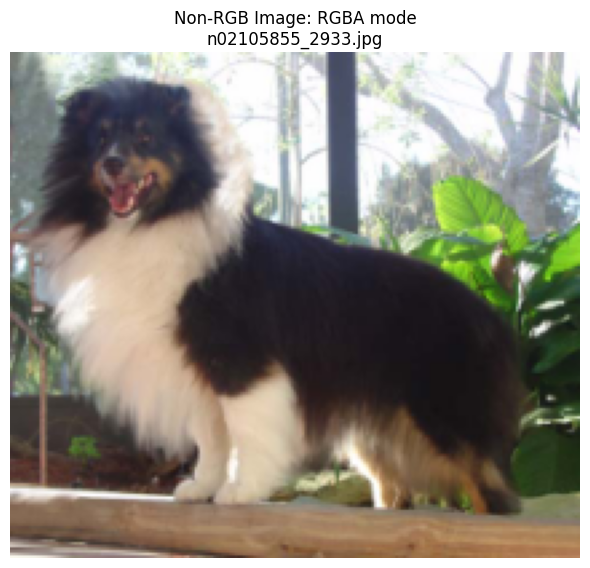
\includegraphics[keepaspectratio]{main_files/figure-pdf/cell-4-output-1.png}}

\begin{verbatim}

   Decision: The 1 RGBA image will be automatically converted to RGB
   during data loading (see data_loader.py). No manual fixing needed.
   This is better than modifying raw data files.
\end{verbatim}

\begin{Shaded}
\begin{Highlighting}[]
\CommentTok{\# Step 5: Extreme aspect ratios}
\NormalTok{scan\_df[}\StringTok{\textquotesingle{}aspect\_ratio\textquotesingle{}}\NormalTok{] }\OperatorTok{=}\NormalTok{ scan\_df[}\StringTok{\textquotesingle{}width\textquotesingle{}}\NormalTok{] }\OperatorTok{/}\NormalTok{ scan\_df[}\StringTok{\textquotesingle{}height\textquotesingle{}}\NormalTok{]}
\NormalTok{extreme\_ratios }\OperatorTok{=}\NormalTok{ scan\_df[}
\NormalTok{    (scan\_df[}\StringTok{\textquotesingle{}aspect\_ratio\textquotesingle{}}\NormalTok{] }\OperatorTok{\textless{}} \FloatTok{0.2}\NormalTok{) }\OperatorTok{|} 
\NormalTok{    (scan\_df[}\StringTok{\textquotesingle{}aspect\_ratio\textquotesingle{}}\NormalTok{] }\OperatorTok{\textgreater{}} \FloatTok{5.0}\NormalTok{)}
\NormalTok{]}
\BuiltInTok{print}\NormalTok{(}\SpecialStringTok{f"}\CharTok{\textbackslash{}n}\SpecialStringTok{5. Extreme Aspect Ratios (\textless{}0.2 or \textgreater{}5.0): }\SpecialCharTok{\{}\BuiltInTok{len}\NormalTok{(extreme\_ratios)}\SpecialCharTok{\}}\SpecialStringTok{"}\NormalTok{)}
\ControlFlowTok{if} \BuiltInTok{len}\NormalTok{(extreme\_ratios) }\OperatorTok{\textgreater{}} \DecValTok{0}\NormalTok{:}
    \BuiltInTok{print}\NormalTok{(}\StringTok{"   Images with unusual ratios (may need special handling):"}\NormalTok{)}
    \ControlFlowTok{for}\NormalTok{ \_, row }\KeywordTok{in}\NormalTok{ extreme\_ratios.head(}\DecValTok{3}\NormalTok{).iterrows():}
        \BuiltInTok{print}\NormalTok{(}\SpecialStringTok{f"     {-} }\SpecialCharTok{\{}\NormalTok{row[}\StringTok{\textquotesingle{}filename\textquotesingle{}}\NormalTok{]}\SpecialCharTok{\}}\SpecialStringTok{: }\SpecialCharTok{\{}\NormalTok{row[}\StringTok{\textquotesingle{}aspect\_ratio\textquotesingle{}}\NormalTok{]}\SpecialCharTok{:.2f\}}\SpecialStringTok{"}\NormalTok{)}

\CommentTok{\# Final summary}
\BuiltInTok{print}\NormalTok{(}\StringTok{"}\CharTok{\textbackslash{}n}\StringTok{"} \OperatorTok{+} \StringTok{"="}\OperatorTok{*}\DecValTok{60}\NormalTok{)}
\BuiltInTok{print}\NormalTok{(}\StringTok{"CLEANING SUMMARY"}\NormalTok{)}
\BuiltInTok{print}\NormalTok{(}\StringTok{"="}\OperatorTok{*}\DecValTok{60}\NormalTok{)}
\NormalTok{clean\_count }\OperatorTok{=} \BuiltInTok{len}\NormalTok{(scan\_df[scan\_df[}\StringTok{\textquotesingle{}valid\textquotesingle{}}\NormalTok{] }\OperatorTok{==} \VariableTok{True}\NormalTok{])}
\NormalTok{removed }\OperatorTok{=} \BuiltInTok{len}\NormalTok{(scan\_df) }\OperatorTok{{-}}\NormalTok{ clean\_count}
\BuiltInTok{print}\NormalTok{(}\SpecialStringTok{f"Initial images:    }\SpecialCharTok{\{}\BuiltInTok{len}\NormalTok{(scan\_df)}\SpecialCharTok{\}}\SpecialStringTok{"}\NormalTok{)}
\BuiltInTok{print}\NormalTok{(}\SpecialStringTok{f"Removed:           }\SpecialCharTok{\{}\NormalTok{removed}\SpecialCharTok{\}}\SpecialStringTok{"}\NormalTok{)}
\BuiltInTok{print}\NormalTok{(}\SpecialStringTok{f"Clean images:      }\SpecialCharTok{\{}\NormalTok{clean\_count}\SpecialCharTok{\}}\SpecialStringTok{"}\NormalTok{)}
\BuiltInTok{print}\NormalTok{(}\SpecialStringTok{f"Removal rate:      }\SpecialCharTok{\{}\NormalTok{removed}\OperatorTok{/}\BuiltInTok{len}\NormalTok{(scan\_df)}\OperatorTok{*}\DecValTok{100}\SpecialCharTok{:.2f\}}\SpecialStringTok{\%"}\NormalTok{)}
\BuiltInTok{print}\NormalTok{(}\StringTok{"}\CharTok{\textbackslash{}n}\StringTok{✓ Dataset is clean and ready for training!"}\NormalTok{)}
\end{Highlighting}
\end{Shaded}

\begin{verbatim}

5. Extreme Aspect Ratios (<0.2 or >5.0): 0

============================================================
CLEANING SUMMARY
============================================================
Initial images:    20580
Removed:           0
Clean images:      20580
Removal rate:      0.00%

✓ Dataset is clean and ready for training!
\end{verbatim}

\subsection{Cleaning Results Summary}\label{cleaning-results-summary}

\textbf{Perfect Dataset Quality} - All 20,580 images passed validation
with zero issues:

\begin{itemize}
\tightlist
\item
  \textbf{0 corrupt images} - All files load successfully
\item
  \textbf{0 duplicates} - No data leakage risk\\
\item
  \textbf{0 size violations} - All images meet dimension and file size
  requirements
\item
  \textbf{1 RGBA image} - Will be auto-converted to RGB during loading
\end{itemize}

\textbf{Label Indexing Fix Applied}:

The breed mapping assigns \texttt{class\_id} values from 1-120
(human-readable format), but Keras neural networks require 0-indexed
labels (0-119). This is handled automatically in the data loading
pipeline:

\begin{itemize}
\tightlist
\item
  \textbf{Source data}: \texttt{breed\_mapping.csv} has
  \texttt{class\_id} = 1-120
\item
  \textbf{Training pipeline}: \texttt{data\_loader.py} subtracts 1 to
  convert to 0-119
\item
  \textbf{Implementation}: See \texttt{data\_loader.py:106} -
  \texttt{return\ img\_array,\ row{[}\textquotesingle{}class\_id\textquotesingle{}{]}\ -\ 1,\ breed\_name}
\end{itemize}

This ensures compatibility with Keras while keeping human-readable breed
mappings in the raw data.

\textbf{Conclusion:} The dataset is exceptionally clean and ready for
the data loading pipeline.

\section{Exploratory Data Analysis}\label{exploratory-data-analysis}

In this section, we explore the dataset characteristics to understand:

\begin{enumerate}
\def\labelenumi{\arabic{enumi}.}
\tightlist
\item
  \textbf{Sample images}: Visual inspection of different breeds
\item
  \textbf{Class distribution}: How balanced are the 120 breed classes?
\item
  \textbf{Image dimensions}: Variation in image sizes and aspect ratios
\item
  \textbf{Data quality}: Any patterns or issues to address before
  training
\end{enumerate}

\begin{Shaded}
\begin{Highlighting}[]
\CommentTok{\# Visualize sample images from different breeds}
\KeywordTok{def}\NormalTok{ show\_sample\_images(train\_df, n\_breeds}\OperatorTok{=}\DecValTok{4}\NormalTok{, images\_per\_breed}\OperatorTok{=}\DecValTok{3}\NormalTok{):}
    \CommentTok{"""Display sample images from random breeds"""}
    
    \CommentTok{\# Sample random breeds}
\NormalTok{    breeds }\OperatorTok{=}\NormalTok{ train\_df[}\StringTok{\textquotesingle{}breed\_name\textquotesingle{}}\NormalTok{].unique()}
\NormalTok{    sample\_breeds }\OperatorTok{=}\NormalTok{ np.random.choice(breeds, }
\NormalTok{                                     size}\OperatorTok{=}\BuiltInTok{min}\NormalTok{(n\_breeds, }\BuiltInTok{len}\NormalTok{(breeds)), replace}\OperatorTok{=}\VariableTok{False}\NormalTok{)}
    
\NormalTok{    fig, axes }\OperatorTok{=}\NormalTok{ plt.subplots(n\_breeds, images\_per\_breed, figsize}\OperatorTok{=}\NormalTok{(}\DecValTok{12}\NormalTok{, n\_breeds}\OperatorTok{*}\DecValTok{3}\NormalTok{))}
    
    \ControlFlowTok{for}\NormalTok{ i, breed }\KeywordTok{in} \BuiltInTok{enumerate}\NormalTok{(sample\_breeds):}
\NormalTok{        breed\_images }\OperatorTok{=}\NormalTok{ train\_df[train\_df[}\StringTok{\textquotesingle{}breed\_name\textquotesingle{}}\NormalTok{] }
                                \OperatorTok{==}\NormalTok{ breed].sample(n}\OperatorTok{=}\NormalTok{images\_per\_breed)}
        
        \ControlFlowTok{for}\NormalTok{ j, (\_, row) }\KeywordTok{in} \BuiltInTok{enumerate}\NormalTok{(breed\_images.iterrows()):}
            \CommentTok{\# Use absolute\_path which has full path from project root}
\NormalTok{            img\_path }\OperatorTok{=}\NormalTok{ Path(}\StringTok{".."}\NormalTok{) }\OperatorTok{/} \StringTok{"data"} \OperatorTok{/} \StringTok{"raw"} \OperatorTok{/}\NormalTok{ row[}\StringTok{\textquotesingle{}file\_path\textquotesingle{}}\NormalTok{]}
\NormalTok{            img }\OperatorTok{=}\NormalTok{ Image.}\BuiltInTok{open}\NormalTok{(img\_path)}
            
\NormalTok{            ax }\OperatorTok{=}\NormalTok{ axes[i, j] }\ControlFlowTok{if}\NormalTok{ n\_breeds }\OperatorTok{\textgreater{}} \DecValTok{1} \ControlFlowTok{else}\NormalTok{ axes[j]}
\NormalTok{            ax.imshow(img)}
\NormalTok{            ax.axis(}\StringTok{\textquotesingle{}off\textquotesingle{}}\NormalTok{)}
            
            \ControlFlowTok{if}\NormalTok{ j }\OperatorTok{==} \DecValTok{0}\NormalTok{:}
\NormalTok{                ax.set\_title(}\SpecialStringTok{f"}\SpecialCharTok{\{}\NormalTok{breed}\SpecialCharTok{\}}\CharTok{\textbackslash{}n}\SpecialCharTok{\{}\NormalTok{img}\SpecialCharTok{.}\NormalTok{size[}\DecValTok{0}\NormalTok{]}\SpecialCharTok{\}}\SpecialStringTok{×}\SpecialCharTok{\{}\NormalTok{img}\SpecialCharTok{.}\NormalTok{size[}\DecValTok{1}\NormalTok{]}\SpecialCharTok{\}}\SpecialStringTok{"}\NormalTok{, fontsize}\OperatorTok{=}\DecValTok{10}\NormalTok{)}
            \ControlFlowTok{else}\NormalTok{:}
\NormalTok{                ax.set\_title(}\SpecialStringTok{f"}\SpecialCharTok{\{}\NormalTok{img}\SpecialCharTok{.}\NormalTok{size[}\DecValTok{0}\NormalTok{]}\SpecialCharTok{\}}\SpecialStringTok{×}\SpecialCharTok{\{}\NormalTok{img}\SpecialCharTok{.}\NormalTok{size[}\DecValTok{1}\NormalTok{]}\SpecialCharTok{\}}\SpecialStringTok{"}\NormalTok{, fontsize}\OperatorTok{=}\DecValTok{9}\NormalTok{)}
    
\NormalTok{    plt.tight\_layout()}
\NormalTok{    plt.savefig(}\StringTok{"../artifacts/figures/sample\_images.png"}\NormalTok{, }
\NormalTok{                dpi}\OperatorTok{=}\DecValTok{150}\NormalTok{, bbox\_inches}\OperatorTok{=}\StringTok{\textquotesingle{}tight\textquotesingle{}}\NormalTok{)}
\NormalTok{    plt.show()}

\CommentTok{\# Create figures directory}
\NormalTok{Path(}\StringTok{"../artifacts/figures"}\NormalTok{).mkdir(parents}\OperatorTok{=}\VariableTok{True}\NormalTok{, exist\_ok}\OperatorTok{=}\VariableTok{True}\NormalTok{)}

\CommentTok{\# Show samples}
\NormalTok{np.random.seed(}\DecValTok{42}\NormalTok{)}
\NormalTok{show\_sample\_images(train\_df, n\_breeds}\OperatorTok{=}\DecValTok{4}\NormalTok{, images\_per\_breed}\OperatorTok{=}\DecValTok{3}\NormalTok{)}
\end{Highlighting}
\end{Shaded}

\pandocbounded{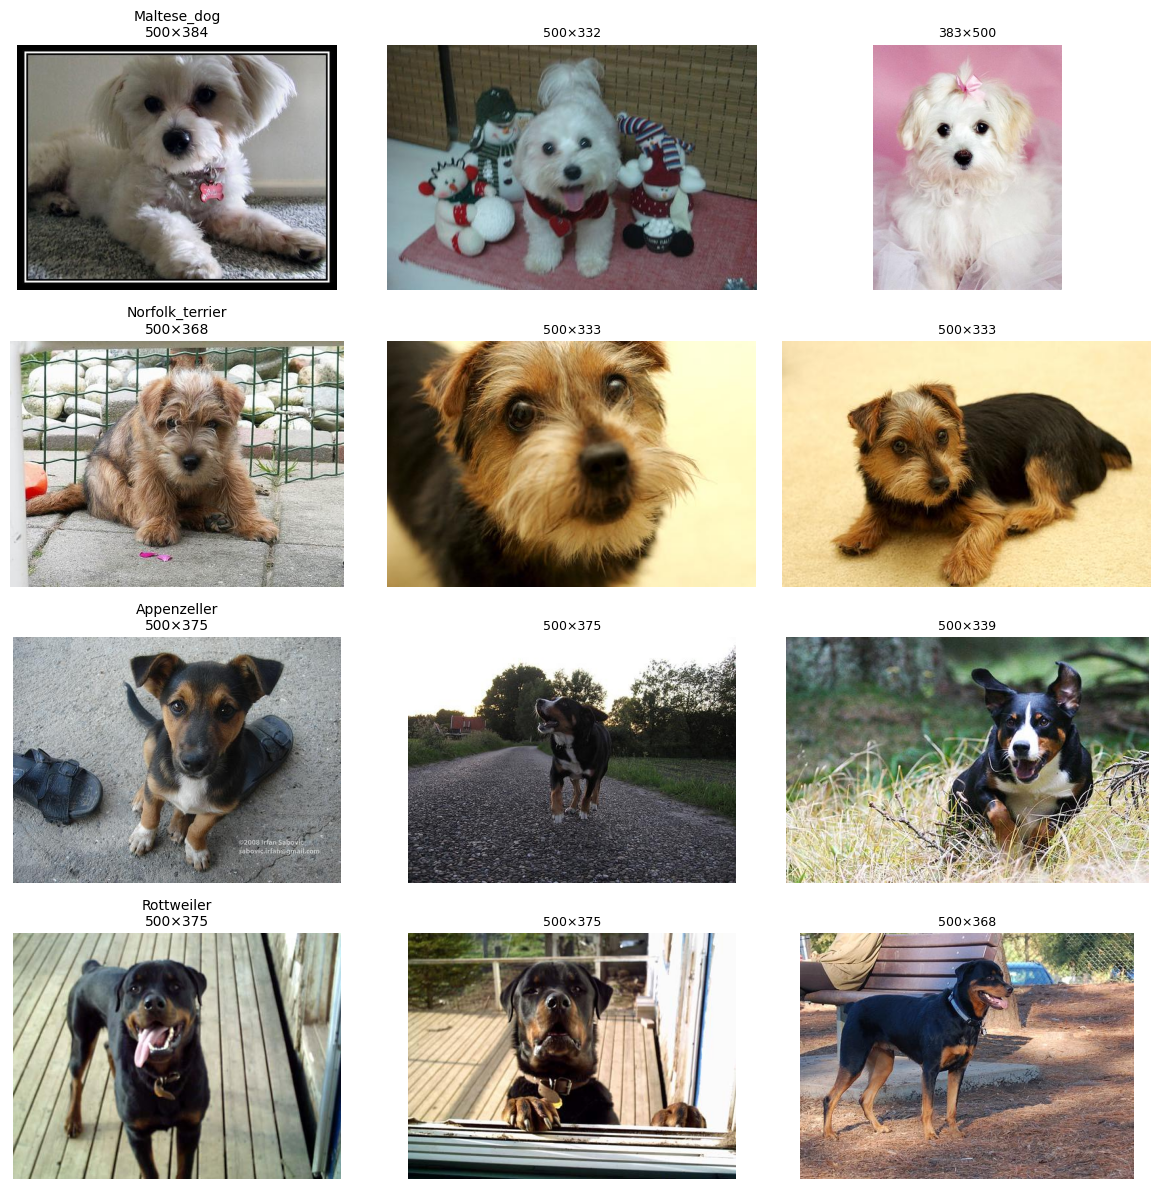
\includegraphics[keepaspectratio]{main_files/figure-pdf/cell-6-output-1.png}}

Sample images showing variety in:

\begin{itemize}
\tightlist
\item
  Breed appearance (different sizes, coat colors, facial features)
\item
  Image dimensions (various aspect ratios and resolutions)
\item
  Photography conditions (backgrounds, lighting, angles)
\end{itemize}

\subsection{Image Dimension Analysis}\label{image-dimension-analysis}

Understanding image sizes helps us choose appropriate preprocessing
strategies

\begin{Shaded}
\begin{Highlighting}[]
\CommentTok{\# Analyze image dimensions}
\NormalTok{fig, axes }\OperatorTok{=}\NormalTok{ plt.subplots(}\DecValTok{1}\NormalTok{, }\DecValTok{3}\NormalTok{, figsize}\OperatorTok{=}\NormalTok{(}\DecValTok{18}\NormalTok{, }\DecValTok{5}\NormalTok{))}

\CommentTok{\# Width distribution}
\NormalTok{axes[}\DecValTok{0}\NormalTok{].hist(train\_df[}\StringTok{\textquotesingle{}width\textquotesingle{}}\NormalTok{], bins}\OperatorTok{=}\DecValTok{50}\NormalTok{, edgecolor}\OperatorTok{=}\StringTok{\textquotesingle{}black\textquotesingle{}}\NormalTok{, alpha}\OperatorTok{=}\FloatTok{0.7}\NormalTok{)}
\NormalTok{axes[}\DecValTok{0}\NormalTok{].axvline(train\_df[}\StringTok{\textquotesingle{}width\textquotesingle{}}\NormalTok{].mean(), color}\OperatorTok{=}\StringTok{\textquotesingle{}red\textquotesingle{}}\NormalTok{, linestyle}\OperatorTok{=}\StringTok{\textquotesingle{}{-}{-}\textquotesingle{}}\NormalTok{,}
\NormalTok{                   label}\OperatorTok{=}\SpecialStringTok{f\textquotesingle{}Mean: }\SpecialCharTok{\{}\NormalTok{train\_df[}\StringTok{"width"}\NormalTok{]}\SpecialCharTok{.}\NormalTok{mean()}\SpecialCharTok{:.0f\}}\SpecialStringTok{\textquotesingle{}}\NormalTok{)}
\NormalTok{axes[}\DecValTok{0}\NormalTok{].set\_xlabel(}\StringTok{\textquotesingle{}Width (pixels)\textquotesingle{}}\NormalTok{)}
\NormalTok{axes[}\DecValTok{0}\NormalTok{].set\_ylabel(}\StringTok{\textquotesingle{}Frequency\textquotesingle{}}\NormalTok{)}
\NormalTok{axes[}\DecValTok{0}\NormalTok{].set\_title(}\StringTok{\textquotesingle{}Image Width Distribution\textquotesingle{}}\NormalTok{)}
\NormalTok{axes[}\DecValTok{0}\NormalTok{].legend()}
\NormalTok{axes[}\DecValTok{0}\NormalTok{].grid(alpha}\OperatorTok{=}\FloatTok{0.3}\NormalTok{)}

\CommentTok{\# Height distribution}
\NormalTok{axes[}\DecValTok{1}\NormalTok{].hist(train\_df[}\StringTok{\textquotesingle{}height\textquotesingle{}}\NormalTok{], bins}\OperatorTok{=}\DecValTok{50}\NormalTok{, edgecolor}\OperatorTok{=}\StringTok{\textquotesingle{}black\textquotesingle{}}\NormalTok{, alpha}\OperatorTok{=}\FloatTok{0.7}\NormalTok{)}
\NormalTok{axes[}\DecValTok{1}\NormalTok{].axvline(train\_df[}\StringTok{\textquotesingle{}height\textquotesingle{}}\NormalTok{].mean(), color}\OperatorTok{=}\StringTok{\textquotesingle{}red\textquotesingle{}}\NormalTok{, linestyle}\OperatorTok{=}\StringTok{\textquotesingle{}{-}{-}\textquotesingle{}}\NormalTok{,}
\NormalTok{                   label}\OperatorTok{=}\SpecialStringTok{f\textquotesingle{}Mean: }\SpecialCharTok{\{}\NormalTok{train\_df[}\StringTok{"height"}\NormalTok{]}\SpecialCharTok{.}\NormalTok{mean()}\SpecialCharTok{:.0f\}}\SpecialStringTok{\textquotesingle{}}\NormalTok{)}
\NormalTok{axes[}\DecValTok{1}\NormalTok{].set\_xlabel(}\StringTok{\textquotesingle{}Height (pixels)\textquotesingle{}}\NormalTok{)}
\NormalTok{axes[}\DecValTok{1}\NormalTok{].set\_ylabel(}\StringTok{\textquotesingle{}Frequency\textquotesingle{}}\NormalTok{)}
\NormalTok{axes[}\DecValTok{1}\NormalTok{].set\_title(}\StringTok{\textquotesingle{}Image Height Distribution\textquotesingle{}}\NormalTok{)}
\NormalTok{axes[}\DecValTok{1}\NormalTok{].legend()}
\NormalTok{axes[}\DecValTok{1}\NormalTok{].grid(alpha}\OperatorTok{=}\FloatTok{0.3}\NormalTok{)}

\CommentTok{\# Aspect ratio}
\NormalTok{train\_df[}\StringTok{\textquotesingle{}aspect\_ratio\textquotesingle{}}\NormalTok{] }\OperatorTok{=}\NormalTok{ train\_df[}\StringTok{\textquotesingle{}width\textquotesingle{}}\NormalTok{] }\OperatorTok{/}\NormalTok{ train\_df[}\StringTok{\textquotesingle{}height\textquotesingle{}}\NormalTok{]}
\NormalTok{axes[}\DecValTok{2}\NormalTok{].hist(train\_df[}\StringTok{\textquotesingle{}aspect\_ratio\textquotesingle{}}\NormalTok{], bins}\OperatorTok{=}\DecValTok{50}\NormalTok{, edgecolor}\OperatorTok{=}\StringTok{\textquotesingle{}black\textquotesingle{}}\NormalTok{, alpha}\OperatorTok{=}\FloatTok{0.7}\NormalTok{)}
\NormalTok{axes[}\DecValTok{2}\NormalTok{].axvline(}\FloatTok{1.0}\NormalTok{, color}\OperatorTok{=}\StringTok{\textquotesingle{}green\textquotesingle{}}\NormalTok{, linestyle}\OperatorTok{=}\StringTok{\textquotesingle{}{-}{-}\textquotesingle{}}\NormalTok{, label}\OperatorTok{=}\StringTok{\textquotesingle{}Square (1:1)\textquotesingle{}}\NormalTok{)}
\NormalTok{axes[}\DecValTok{2}\NormalTok{].set\_xlabel(}\StringTok{\textquotesingle{}Aspect Ratio (width/height)\textquotesingle{}}\NormalTok{)}
\NormalTok{axes[}\DecValTok{2}\NormalTok{].set\_ylabel(}\StringTok{\textquotesingle{}Frequency\textquotesingle{}}\NormalTok{)}
\NormalTok{axes[}\DecValTok{2}\NormalTok{].set\_title(}\StringTok{\textquotesingle{}Aspect Ratio Distribution\textquotesingle{}}\NormalTok{)}
\NormalTok{axes[}\DecValTok{2}\NormalTok{].legend()}
\NormalTok{axes[}\DecValTok{2}\NormalTok{].grid(alpha}\OperatorTok{=}\FloatTok{0.3}\NormalTok{)}
\end{Highlighting}
\end{Shaded}

\pandocbounded{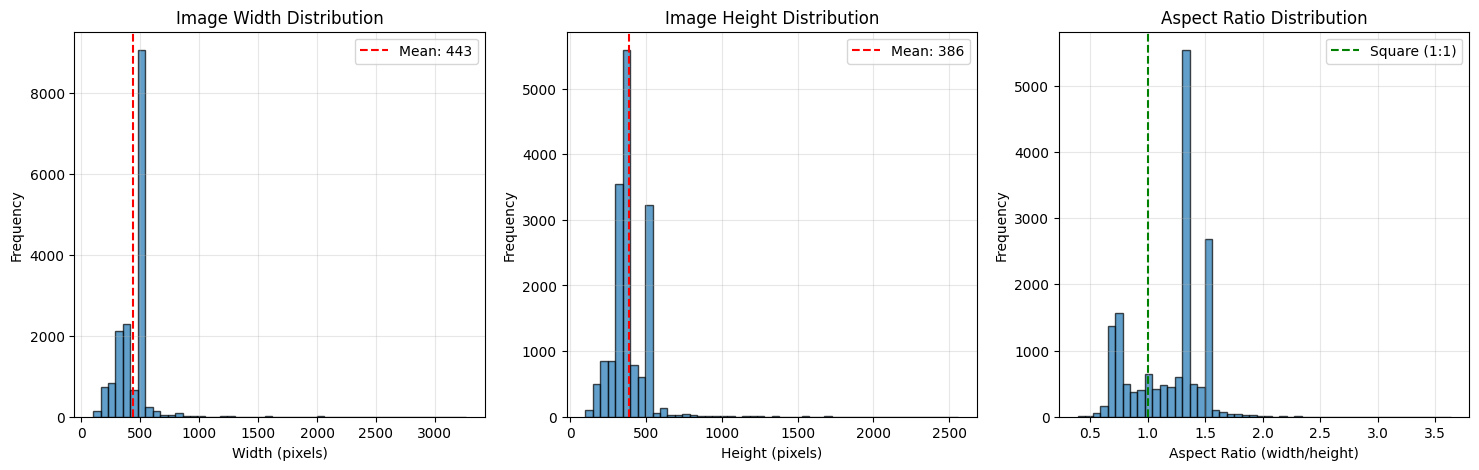
\includegraphics[keepaspectratio]{main_files/figure-pdf/cell-7-output-1.png}}

\begin{Shaded}
\begin{Highlighting}[]
\CommentTok{\# Scatter: width vs height}
\NormalTok{fig, ax }\OperatorTok{=}\NormalTok{ plt.subplots(}\DecValTok{1}\NormalTok{, }\DecValTok{1}\NormalTok{, figsize}\OperatorTok{=}\NormalTok{(}\DecValTok{8}\NormalTok{, }\DecValTok{6}\NormalTok{))}

\NormalTok{ax.scatter(train\_df[}\StringTok{\textquotesingle{}width\textquotesingle{}}\NormalTok{], train\_df[}\StringTok{\textquotesingle{}height\textquotesingle{}}\NormalTok{], alpha}\OperatorTok{=}\FloatTok{0.3}\NormalTok{, s}\OperatorTok{=}\DecValTok{1}\NormalTok{)}
\NormalTok{ax.plot([}\DecValTok{0}\NormalTok{, }\DecValTok{1000}\NormalTok{], [}\DecValTok{0}\NormalTok{, }\DecValTok{1000}\NormalTok{], }\StringTok{\textquotesingle{}r{-}{-}\textquotesingle{}}\NormalTok{, label}\OperatorTok{=}\StringTok{\textquotesingle{}Square\textquotesingle{}}\NormalTok{, linewidth}\OperatorTok{=}\DecValTok{1}\NormalTok{)}
\NormalTok{ax.set\_xlabel(}\StringTok{\textquotesingle{}Width (pixels)\textquotesingle{}}\NormalTok{)}
\NormalTok{ax.set\_ylabel(}\StringTok{\textquotesingle{}Height (pixels)\textquotesingle{}}\NormalTok{)}
\NormalTok{ax.set\_title(}\StringTok{\textquotesingle{}Width vs Height Scatter\textquotesingle{}}\NormalTok{)}
\NormalTok{ax.legend()}
\NormalTok{ax.grid(alpha}\OperatorTok{=}\FloatTok{0.3}\NormalTok{)}
\NormalTok{ax.set\_xlim(}\DecValTok{0}\NormalTok{, train\_df[}\StringTok{\textquotesingle{}width\textquotesingle{}}\NormalTok{].}\BuiltInTok{max}\NormalTok{() }\OperatorTok{+} \DecValTok{50}\NormalTok{)}
\NormalTok{ax.set\_ylim(}\DecValTok{0}\NormalTok{, train\_df[}\StringTok{\textquotesingle{}height\textquotesingle{}}\NormalTok{].}\BuiltInTok{max}\NormalTok{() }\OperatorTok{+} \DecValTok{50}\NormalTok{)}

\NormalTok{plt.tight\_layout()}
\NormalTok{plt.savefig(}\StringTok{"../artifacts/figures/image\_dimensions\_scatter.png"}\NormalTok{, }
\NormalTok{            dpi}\OperatorTok{=}\DecValTok{150}\NormalTok{, bbox\_inches}\OperatorTok{=}\StringTok{\textquotesingle{}tight\textquotesingle{}}\NormalTok{)}
\NormalTok{plt.show()}
\end{Highlighting}
\end{Shaded}

\pandocbounded{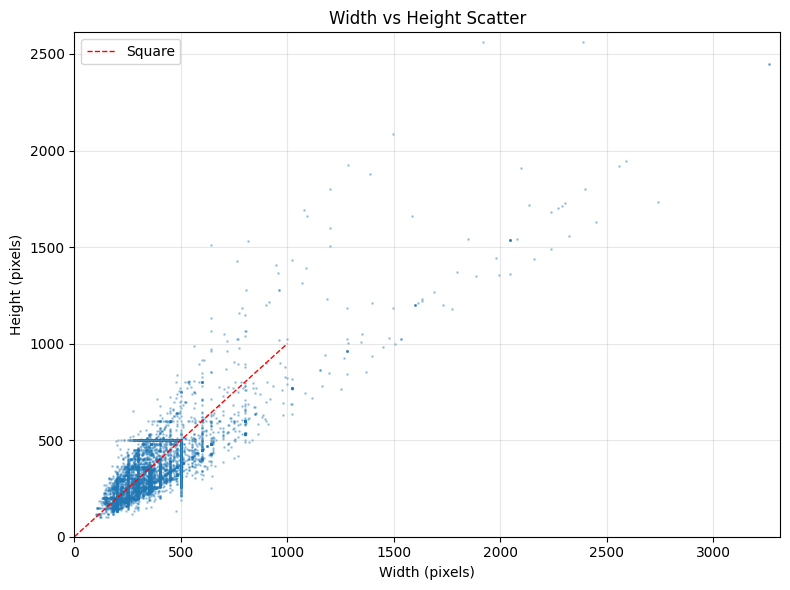
\includegraphics[keepaspectratio]{main_files/figure-pdf/cell-8-output-1.png}}

\textbf{Key Findings:}

\textbf{Highly Variable Dimensions}: Images range from 100×100 to
3264×2562 pixels with mean 443×386

\begin{itemize}
\tightlist
\item
  \textbf{Width}: Mean 443px (±145), Range {[}100, 3264{]}
\item
  \textbf{Height}: Mean 386px (±127), Range {[}100, 2562{]}\\
\item
  \textbf{Aspect Ratio}: Mean 1.19 (±0.30), mostly landscape orientation
\end{itemize}

\textbf{Low-Resolution Images}: Some images will require upscaling

\begin{itemize}
\tightlist
\item
  Resizing 100×100 → 224×224 requires 2.2× upscaling (will be blurry)
\item
  Most images (mean \textasciitilde440×390) will be downscaled,
  preserving quality
\item
  Low-res images may be harder for the model to classify accurately
\end{itemize}

\textbf{Preprocessing Decision}: Resizing to 224×224 is appropriate
since:

\begin{itemize}
\tightlist
\item
  Most images are already close to this size (reduces distortion)
\item
  Standard for ImageNet pre-trained models (ResNet, VGG, EfficientNet)
\item
  Square format normalizes the varying aspect ratios
\item
  Bilinear interpolation handles both upscaling and downscaling
\end{itemize}

Let us also take a look at the low-resolution images that need
upscaling:

\begin{Shaded}
\begin{Highlighting}[]
\CommentTok{\# Analyze low{-}resolution images needing upscaling}
\BuiltInTok{print}\NormalTok{(}\StringTok{"Low{-}Resolution Image Analysis"}\NormalTok{)}
\BuiltInTok{print}\NormalTok{(}\StringTok{"="}\OperatorTok{*}\DecValTok{60}\NormalTok{)}

\CommentTok{\# Images smaller than target size (224x224)}
\NormalTok{needs\_upscale }\OperatorTok{=}\NormalTok{ train\_df[}
\NormalTok{    (train\_df[}\StringTok{\textquotesingle{}width\textquotesingle{}}\NormalTok{] }\OperatorTok{\textless{}} \DecValTok{224}\NormalTok{) }\OperatorTok{|}\NormalTok{ (train\_df[}\StringTok{\textquotesingle{}height\textquotesingle{}}\NormalTok{] }\OperatorTok{\textless{}} \DecValTok{224}\NormalTok{)}
\NormalTok{]}
\NormalTok{n\_total }\OperatorTok{=} \BuiltInTok{len}\NormalTok{(train\_df)}
\NormalTok{n\_small }\OperatorTok{=} \BuiltInTok{len}\NormalTok{(needs\_upscale)}
\NormalTok{pct\_small }\OperatorTok{=}\NormalTok{ n\_small }\OperatorTok{/}\NormalTok{ n\_total }\OperatorTok{*} \DecValTok{100}

\BuiltInTok{print}\NormalTok{(}\SpecialStringTok{f"}\CharTok{\textbackslash{}n}\SpecialStringTok{Images requiring upscaling: }\SpecialCharTok{\{}\NormalTok{n\_small}\SpecialCharTok{\}}\SpecialStringTok{ / }\SpecialCharTok{\{}\NormalTok{n\_total}\SpecialCharTok{\}}\SpecialStringTok{"}\NormalTok{)}
\BuiltInTok{print}\NormalTok{(}\SpecialStringTok{f"  Percentage: }\SpecialCharTok{\{}\NormalTok{pct\_small}\SpecialCharTok{:.1f\}}\SpecialStringTok{\%"}\NormalTok{)}

\CommentTok{\# Break down by severity}
\NormalTok{very\_small }\OperatorTok{=}\NormalTok{ train\_df[}
\NormalTok{    (train\_df[}\StringTok{\textquotesingle{}width\textquotesingle{}}\NormalTok{] }\OperatorTok{\textless{}} \DecValTok{150}\NormalTok{) }\OperatorTok{\&}\NormalTok{ (train\_df[}\StringTok{\textquotesingle{}height\textquotesingle{}}\NormalTok{] }\OperatorTok{\textless{}} \DecValTok{150}\NormalTok{)}
\NormalTok{]}
\NormalTok{small }\OperatorTok{=}\NormalTok{ train\_df[}
\NormalTok{    ((train\_df[}\StringTok{\textquotesingle{}width\textquotesingle{}}\NormalTok{] }\OperatorTok{\textgreater{}=} \DecValTok{150}\NormalTok{) }\OperatorTok{\&}\NormalTok{ (train\_df[}\StringTok{\textquotesingle{}width\textquotesingle{}}\NormalTok{] }\OperatorTok{\textless{}} \DecValTok{224}\NormalTok{)) }\OperatorTok{|}
\NormalTok{    ((train\_df[}\StringTok{\textquotesingle{}height\textquotesingle{}}\NormalTok{] }\OperatorTok{\textgreater{}=} \DecValTok{150}\NormalTok{) }\OperatorTok{\&}\NormalTok{ (train\_df[}\StringTok{\textquotesingle{}height\textquotesingle{}}\NormalTok{] }\OperatorTok{\textless{}} \DecValTok{224}\NormalTok{))}
\NormalTok{]}

\NormalTok{n\_very\_small }\OperatorTok{=} \BuiltInTok{len}\NormalTok{(very\_small)}
\NormalTok{n\_sm }\OperatorTok{=} \BuiltInTok{len}\NormalTok{(small)}
\BuiltInTok{print}\NormalTok{(}\SpecialStringTok{f"  {-} Very small (\textless{}150×150): }\SpecialCharTok{\{}\NormalTok{n\_very\_small}\SpecialCharTok{\}}\SpecialStringTok{ images"}\NormalTok{)}
\BuiltInTok{print}\NormalTok{(}\SpecialStringTok{f"     (}\SpecialCharTok{\{}\NormalTok{n\_very\_small}\OperatorTok{/}\NormalTok{n\_total}\OperatorTok{*}\DecValTok{100}\SpecialCharTok{:.2f\}}\SpecialStringTok{\%)"}\NormalTok{)}
\BuiltInTok{print}\NormalTok{(}\SpecialStringTok{f"  {-} Small (150{-}224): }\SpecialCharTok{\{}\NormalTok{n\_sm}\SpecialCharTok{\}}\SpecialStringTok{ images"}\NormalTok{)}
\BuiltInTok{print}\NormalTok{(}\SpecialStringTok{f"     (}\SpecialCharTok{\{}\NormalTok{n\_sm}\OperatorTok{/}\NormalTok{n\_total}\OperatorTok{*}\DecValTok{100}\SpecialCharTok{:.2f\}}\SpecialStringTok{\%)"}\NormalTok{)}
\end{Highlighting}
\end{Shaded}

\begin{verbatim}
Low-Resolution Image Analysis
============================================================

Images requiring upscaling: 1261 / 16508
  Percentage: 7.6%
  - Very small (<150×150): 15 images
     (0.09%)
  - Small (150-224): 1233 images
     (7.47%)
\end{verbatim}

\begin{Shaded}
\begin{Highlighting}[]
\CommentTok{\# Find the smallest images}
\BuiltInTok{print}\NormalTok{(}\SpecialStringTok{f"}\CharTok{\textbackslash{}n}\SpecialStringTok{Smallest images:"}\NormalTok{)}
\NormalTok{smallest }\OperatorTok{=}\NormalTok{ train\_df.nsmallest(}\DecValTok{5}\NormalTok{, [}\StringTok{\textquotesingle{}width\textquotesingle{}}\NormalTok{, }\StringTok{\textquotesingle{}height\textquotesingle{}}\NormalTok{])}
\ControlFlowTok{for}\NormalTok{ \_, row }\KeywordTok{in}\NormalTok{ smallest.iterrows():}
\NormalTok{    fname }\OperatorTok{=}\NormalTok{ row[}\StringTok{\textquotesingle{}filename\textquotesingle{}}\NormalTok{]}
\NormalTok{    w, h }\OperatorTok{=}\NormalTok{ row[}\StringTok{\textquotesingle{}width\textquotesingle{}}\NormalTok{], row[}\StringTok{\textquotesingle{}height\textquotesingle{}}\NormalTok{]}
\NormalTok{    breed }\OperatorTok{=}\NormalTok{ row[}\StringTok{\textquotesingle{}breed\_name\textquotesingle{}}\NormalTok{]}
    \BuiltInTok{print}\NormalTok{(}\SpecialStringTok{f"  }\SpecialCharTok{\{}\NormalTok{fname}\SpecialCharTok{\}}\SpecialStringTok{: }\SpecialCharTok{\{}\NormalTok{w}\SpecialCharTok{\}}\SpecialStringTok{×}\SpecialCharTok{\{}\NormalTok{h}\SpecialCharTok{\}}\SpecialStringTok{ {-} }\SpecialCharTok{\{}\NormalTok{breed}\SpecialCharTok{\}}\SpecialStringTok{"}\NormalTok{)}

\CommentTok{\# Visualize upscaling effect on small images}
\NormalTok{fig, axes }\OperatorTok{=}\NormalTok{ plt.subplots(}\DecValTok{2}\NormalTok{, }\DecValTok{3}\NormalTok{, figsize}\OperatorTok{=}\NormalTok{(}\DecValTok{15}\NormalTok{, }\DecValTok{10}\NormalTok{))}

\CommentTok{\# Show 3 small images: original vs resized}
\NormalTok{sample\_imgs }\OperatorTok{=}\NormalTok{ needs\_upscale.sample(}
\NormalTok{    n}\OperatorTok{=}\BuiltInTok{min}\NormalTok{(}\DecValTok{3}\NormalTok{, }\BuiltInTok{len}\NormalTok{(needs\_upscale)), }
\NormalTok{    random\_state}\OperatorTok{=}\DecValTok{42}
\NormalTok{)}

\ControlFlowTok{for}\NormalTok{ i, (\_, row) }\KeywordTok{in} \BuiltInTok{enumerate}\NormalTok{(sample\_imgs.iterrows()):}
\NormalTok{    img\_path }\OperatorTok{=}\NormalTok{ Path(}\StringTok{".."}\NormalTok{) }\OperatorTok{/} \StringTok{"data"} \OperatorTok{/} \StringTok{"raw"} \OperatorTok{/}\NormalTok{ row[}\StringTok{\textquotesingle{}file\_path\textquotesingle{}}\NormalTok{]}
\NormalTok{    img\_orig }\OperatorTok{=}\NormalTok{ Image.}\BuiltInTok{open}\NormalTok{(img\_path).convert(}\StringTok{\textquotesingle{}RGB\textquotesingle{}}\NormalTok{)}
\NormalTok{    img\_resized }\OperatorTok{=}\NormalTok{ img\_orig.resize((}\DecValTok{224}\NormalTok{, }\DecValTok{224}\NormalTok{), Image.BILINEAR)}
    
    \CommentTok{\# Original}
\NormalTok{    axes[}\DecValTok{0}\NormalTok{, i].imshow(img\_orig)}
\NormalTok{    w, h }\OperatorTok{=}\NormalTok{ img\_orig.size}
\NormalTok{    breed }\OperatorTok{=}\NormalTok{ row[}\StringTok{\textquotesingle{}breed\_name\textquotesingle{}}\NormalTok{]}
\NormalTok{    title\_orig }\OperatorTok{=} \SpecialStringTok{f"Original: }\SpecialCharTok{\{}\NormalTok{w}\SpecialCharTok{\}}\SpecialStringTok{×}\SpecialCharTok{\{}\NormalTok{h}\SpecialCharTok{\}}\CharTok{\textbackslash{}n}\SpecialCharTok{\{}\NormalTok{breed}\SpecialCharTok{\}}\SpecialStringTok{"}
\NormalTok{    axes[}\DecValTok{0}\NormalTok{, i].set\_title(title\_orig, fontsize}\OperatorTok{=}\DecValTok{9}\NormalTok{)}
\NormalTok{    axes[}\DecValTok{0}\NormalTok{, i].axis(}\StringTok{\textquotesingle{}off\textquotesingle{}}\NormalTok{)}
    
    \CommentTok{\# Resized}
\NormalTok{    axes[}\DecValTok{1}\NormalTok{, i].imshow(img\_resized)}
\NormalTok{    scale\_factor }\OperatorTok{=} \DecValTok{224} \OperatorTok{/} \BuiltInTok{min}\NormalTok{(img\_orig.size)}
\NormalTok{    title\_resized }\OperatorTok{=} \SpecialStringTok{f"Resized: 224×224}\CharTok{\textbackslash{}n}\SpecialStringTok{(upscaled }\SpecialCharTok{\{}\NormalTok{scale\_factor}\SpecialCharTok{:.2f\}}\SpecialStringTok{×)"}
\NormalTok{    axes[}\DecValTok{1}\NormalTok{, i].set\_title(title\_resized, fontsize}\OperatorTok{=}\DecValTok{9}\NormalTok{)}
\NormalTok{    axes[}\DecValTok{1}\NormalTok{, i].axis(}\StringTok{\textquotesingle{}off\textquotesingle{}}\NormalTok{)}

\NormalTok{suptitle }\OperatorTok{=} \StringTok{"Low{-}Resolution Images: Original vs Upscaled to 224×224"}
\NormalTok{plt.suptitle(suptitle, fontsize}\OperatorTok{=}\DecValTok{14}\NormalTok{, fontweight}\OperatorTok{=}\StringTok{\textquotesingle{}bold\textquotesingle{}}\NormalTok{)}
\NormalTok{plt.tight\_layout()}
\NormalTok{plt.savefig(}\StringTok{"../artifacts/figures/upscaling\_comparison.png"}\NormalTok{, }
\NormalTok{            dpi}\OperatorTok{=}\DecValTok{150}\NormalTok{, bbox\_inches}\OperatorTok{=}\StringTok{\textquotesingle{}tight\textquotesingle{}}\NormalTok{)}
\NormalTok{plt.show()}

\NormalTok{pct\_upscale }\OperatorTok{=}\NormalTok{ n\_small }\OperatorTok{/}\NormalTok{ n\_total }\OperatorTok{*} \DecValTok{100}
\BuiltInTok{print}\NormalTok{(}\SpecialStringTok{f"}\CharTok{\textbackslash{}n}\SpecialStringTok{✓ Conclusion: Despite }\SpecialCharTok{\{}\NormalTok{pct\_upscale}\SpecialCharTok{:.1f\}}\SpecialStringTok{\% of images"}\NormalTok{)}
\BuiltInTok{print}\NormalTok{(}\SpecialStringTok{f"  requiring upscaling, bilinear interpolation"}\NormalTok{)}
\BuiltInTok{print}\NormalTok{(}\SpecialStringTok{f"  preserves key visual features (breed characteristics,"}\NormalTok{)}
\BuiltInTok{print}\NormalTok{(}\SpecialStringTok{f"  coat patterns, facial structure) sufficiently well"}\NormalTok{)}
\BuiltInTok{print}\NormalTok{(}\SpecialStringTok{f"  for classification. Upscaling quality is acceptable."}\NormalTok{)}
\end{Highlighting}
\end{Shaded}

\begin{verbatim}

Smallest images:
  n02089078_4466.jpg: 100×115 - black-and-tan_coonhound
  n02110627_13453.jpg: 103×120 - affenpinscher
  n02089973_2943.jpg: 106×150 - English_foxhound
  n02089973_243.jpg: 107×150 - English_foxhound
  n02101388_4333.jpg: 108×120 - Brittany_spaniel
\end{verbatim}

\pandocbounded{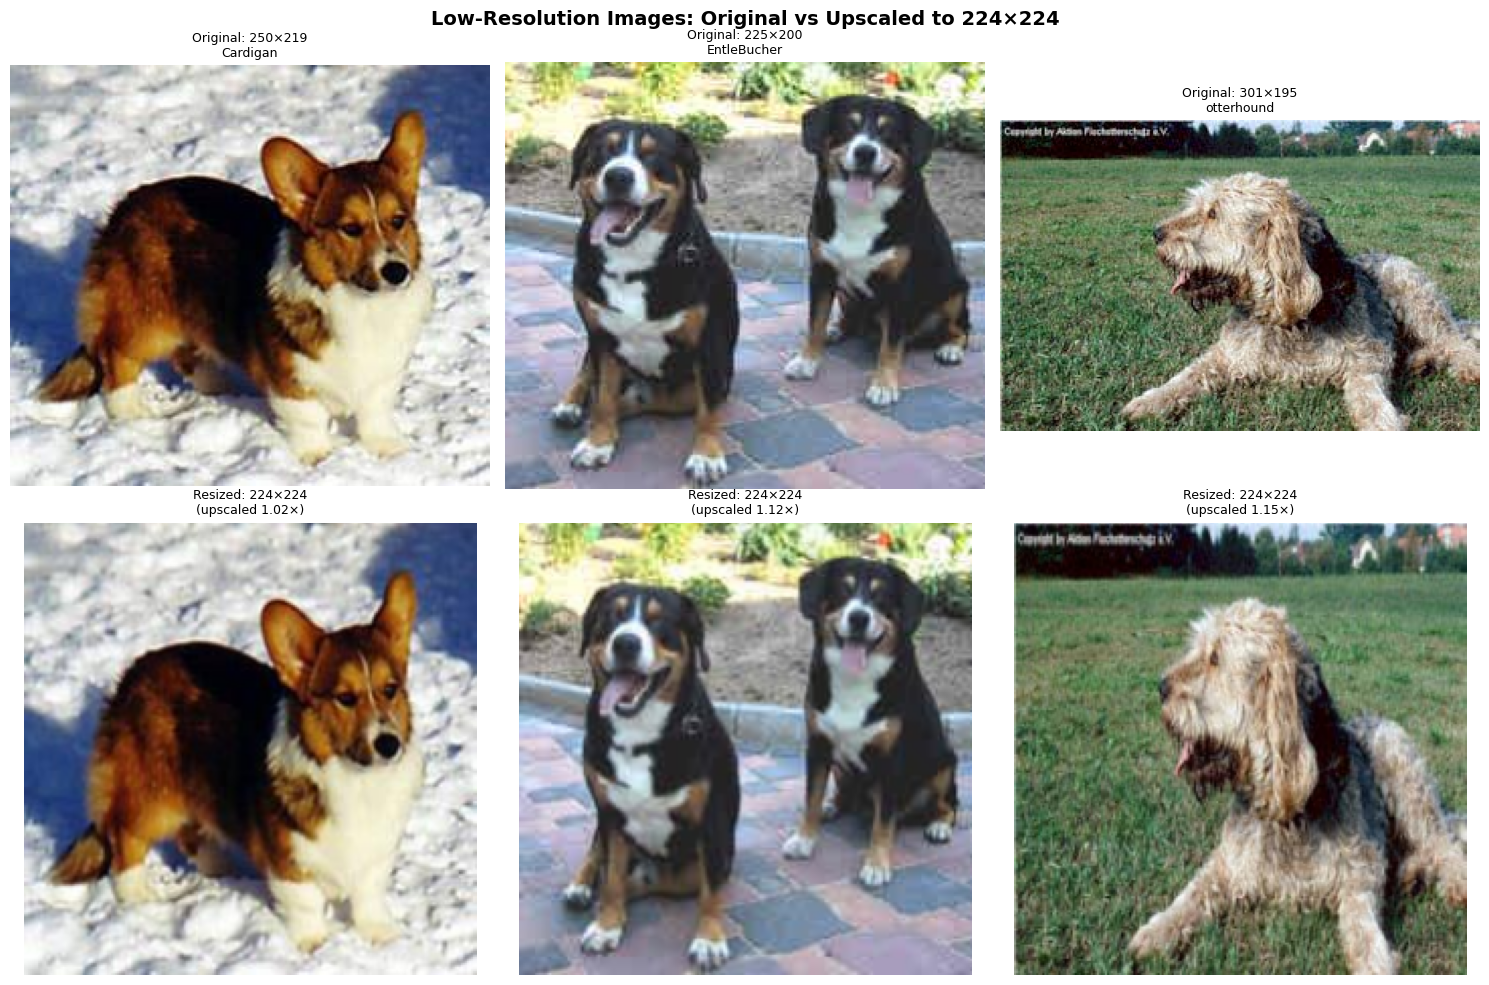
\includegraphics[keepaspectratio]{main_files/figure-pdf/cell-10-output-2.png}}

\begin{verbatim}

✓ Conclusion: Despite 7.6% of images
  requiring upscaling, bilinear interpolation
  preserves key visual features (breed characteristics,
  coat patterns, facial structure) sufficiently well
  for classification. Upscaling quality is acceptable.
\end{verbatim}

\subsection{Class Distribution
Analysis}\label{class-distribution-analysis}

Understanding how balanced our dataset is across the 120 dog breeds
helps us anticipate potential model bias and decide if techniques like
class weighting are needed.

\begin{Shaded}
\begin{Highlighting}[]
\CommentTok{\# Analyze class distribution}
\NormalTok{breed\_counts }\OperatorTok{=}\NormalTok{ train\_df[}\StringTok{\textquotesingle{}breed\_name\textquotesingle{}}\NormalTok{].value\_counts()}
\NormalTok{breed\_counts }\OperatorTok{=}\NormalTok{ breed\_counts.sort\_values(ascending}\OperatorTok{=}\VariableTok{False}\NormalTok{)}

\NormalTok{fig, axes }\OperatorTok{=}\NormalTok{ plt.subplots(}\DecValTok{1}\NormalTok{, }\DecValTok{2}\NormalTok{, figsize}\OperatorTok{=}\NormalTok{(}\DecValTok{16}\NormalTok{, }\DecValTok{5}\NormalTok{))}

\CommentTok{\# Plot 1: Top 20 breeds}
\NormalTok{top20 }\OperatorTok{=}\NormalTok{ breed\_counts.head(}\DecValTok{20}\NormalTok{)}
\NormalTok{axes[}\DecValTok{0}\NormalTok{].barh(top20.index[::}\OperatorTok{{-}}\DecValTok{1}\NormalTok{], top20.values[::}\OperatorTok{{-}}\DecValTok{1}\NormalTok{])}
\NormalTok{axes[}\DecValTok{0}\NormalTok{].set\_xlabel(}\StringTok{\textquotesingle{}Number of Images\textquotesingle{}}\NormalTok{)}
\NormalTok{axes[}\DecValTok{0}\NormalTok{].set\_title(}\StringTok{\textquotesingle{}Top 20 Breeds by Image Count (Training Set)\textquotesingle{}}\NormalTok{)}
\NormalTok{axes[}\DecValTok{0}\NormalTok{].grid(axis}\OperatorTok{=}\StringTok{\textquotesingle{}x\textquotesingle{}}\NormalTok{, alpha}\OperatorTok{=}\FloatTok{0.3}\NormalTok{)}

\CommentTok{\# Plot 2: Distribution histogram}
\NormalTok{axes[}\DecValTok{1}\NormalTok{].hist(breed\_counts.values, bins}\OperatorTok{=}\DecValTok{30}\NormalTok{, }
\NormalTok{             edgecolor}\OperatorTok{=}\StringTok{\textquotesingle{}black\textquotesingle{}}\NormalTok{, alpha}\OperatorTok{=}\FloatTok{0.7}\NormalTok{)}

\NormalTok{mean\_val }\OperatorTok{=}\NormalTok{ breed\_counts.mean()}
\NormalTok{median\_val }\OperatorTok{=}\NormalTok{ breed\_counts.median()}
\NormalTok{axes[}\DecValTok{1}\NormalTok{].axvline(mean\_val, color}\OperatorTok{=}\StringTok{\textquotesingle{}red\textquotesingle{}}\NormalTok{, linestyle}\OperatorTok{=}\StringTok{\textquotesingle{}{-}{-}\textquotesingle{}}\NormalTok{,}
\NormalTok{                label}\OperatorTok{=}\SpecialStringTok{f\textquotesingle{}Mean: }\SpecialCharTok{\{}\NormalTok{mean\_val}\SpecialCharTok{:.1f\}}\SpecialStringTok{\textquotesingle{}}\NormalTok{)}
\NormalTok{axes[}\DecValTok{1}\NormalTok{].axvline(median\_val, color}\OperatorTok{=}\StringTok{\textquotesingle{}green\textquotesingle{}}\NormalTok{, linestyle}\OperatorTok{=}\StringTok{\textquotesingle{}{-}{-}\textquotesingle{}}\NormalTok{,}
\NormalTok{                label}\OperatorTok{=}\SpecialStringTok{f\textquotesingle{}Median: }\SpecialCharTok{\{}\NormalTok{median\_val}\SpecialCharTok{:.1f\}}\SpecialStringTok{\textquotesingle{}}\NormalTok{)}
\NormalTok{axes[}\DecValTok{1}\NormalTok{].set\_xlabel(}\StringTok{\textquotesingle{}Number of Images per Breed\textquotesingle{}}\NormalTok{)}
\NormalTok{axes[}\DecValTok{1}\NormalTok{].set\_ylabel(}\StringTok{\textquotesingle{}Number of Breeds\textquotesingle{}}\NormalTok{)}
\NormalTok{axes[}\DecValTok{1}\NormalTok{].set\_title(}\StringTok{\textquotesingle{}Distribution of Images Across Breeds\textquotesingle{}}\NormalTok{)}
\NormalTok{axes[}\DecValTok{1}\NormalTok{].legend()}
\NormalTok{axes[}\DecValTok{1}\NormalTok{].grid(alpha}\OperatorTok{=}\FloatTok{0.3}\NormalTok{)}

\NormalTok{plt.tight\_layout()}
\NormalTok{plt.savefig(}\StringTok{"../artifacts/figures/breed\_distribution.png"}\NormalTok{, }
\NormalTok{            dpi}\OperatorTok{=}\DecValTok{150}\NormalTok{, bbox\_inches}\OperatorTok{=}\StringTok{\textquotesingle{}tight\textquotesingle{}}\NormalTok{)}

\BuiltInTok{print}\NormalTok{(}\SpecialStringTok{f"}\CharTok{\textbackslash{}n}\SpecialStringTok{Class Balance Analysis:"}\NormalTok{)}
\BuiltInTok{print}\NormalTok{(}\SpecialStringTok{f"  Total breeds: }\SpecialCharTok{\{}\BuiltInTok{len}\NormalTok{(breed\_counts)}\SpecialCharTok{\}}\SpecialStringTok{"}\NormalTok{)}
\BuiltInTok{print}\NormalTok{(}\SpecialStringTok{f"  Min images per breed: }\SpecialCharTok{\{}\NormalTok{breed\_counts}\SpecialCharTok{.}\BuiltInTok{min}\NormalTok{()}\SpecialCharTok{\}}\SpecialStringTok{"}\NormalTok{)}
\BuiltInTok{print}\NormalTok{(}\SpecialStringTok{f"  Max images per breed: }\SpecialCharTok{\{}\NormalTok{breed\_counts}\SpecialCharTok{.}\BuiltInTok{max}\NormalTok{()}\SpecialCharTok{\}}\SpecialStringTok{"}\NormalTok{)}
\BuiltInTok{print}\NormalTok{(}\SpecialStringTok{f"  Mean images per breed: }\SpecialCharTok{\{}\NormalTok{mean\_val}\SpecialCharTok{:.1f\}}\SpecialStringTok{"}\NormalTok{)}
\BuiltInTok{print}\NormalTok{(}\SpecialStringTok{f"  Std images per breed: }\SpecialCharTok{\{}\NormalTok{breed\_counts}\SpecialCharTok{.}\NormalTok{std()}\SpecialCharTok{:.1f\}}\SpecialStringTok{"}\NormalTok{)}

\NormalTok{imbalance\_ratio }\OperatorTok{=}\NormalTok{ breed\_counts.}\BuiltInTok{max}\NormalTok{() }\OperatorTok{/}\NormalTok{ breed\_counts.}\BuiltInTok{min}\NormalTok{()}
\BuiltInTok{print}\NormalTok{(}\SpecialStringTok{f"  Imbalance ratio (max/min): }\SpecialCharTok{\{}\NormalTok{imbalance\_ratio}\SpecialCharTok{:.2f\}}\SpecialStringTok{x"}\NormalTok{)}

\BuiltInTok{print}\NormalTok{(}\SpecialStringTok{f"}\CharTok{\textbackslash{}n}\SpecialStringTok{Most common breeds:"}\NormalTok{)}
\ControlFlowTok{for}\NormalTok{ breed, count }\KeywordTok{in}\NormalTok{ breed\_counts.head(}\DecValTok{5}\NormalTok{).items():}
    \BuiltInTok{print}\NormalTok{(}\SpecialStringTok{f"  }\SpecialCharTok{\{}\NormalTok{breed}\SpecialCharTok{\}}\SpecialStringTok{: }\SpecialCharTok{\{}\NormalTok{count}\SpecialCharTok{\}}\SpecialStringTok{ images"}\NormalTok{)}
    
\BuiltInTok{print}\NormalTok{(}\SpecialStringTok{f"}\CharTok{\textbackslash{}n}\SpecialStringTok{Least common breeds:"}\NormalTok{)}
\ControlFlowTok{for}\NormalTok{ breed, count }\KeywordTok{in}\NormalTok{ breed\_counts.tail(}\DecValTok{5}\NormalTok{).items():}
    \BuiltInTok{print}\NormalTok{(}\SpecialStringTok{f"  }\SpecialCharTok{\{}\NormalTok{breed}\SpecialCharTok{\}}\SpecialStringTok{: }\SpecialCharTok{\{}\NormalTok{count}\SpecialCharTok{\}}\SpecialStringTok{ images"}\NormalTok{)}
\end{Highlighting}
\end{Shaded}

\begin{verbatim}

Class Balance Analysis:
  Total breeds: 120
  Min images per breed: 119
  Max images per breed: 202
  Mean images per breed: 137.6
  Std images per breed: 18.6
  Imbalance ratio (max/min): 1.70x

Most common breeds:
  Maltese_dog: 202 images
  Afghan_hound: 192 images
  Scottish_deerhound: 186 images
  Pomeranian: 176 images
  Samoyed: 175 images

Least common breeds:
  clumber: 120 images
  Border_collie: 120 images
  Pekinese: 120 images
  Bouvier_des_Flandres: 120 images
  redbone: 119 images
\end{verbatim}

\pandocbounded{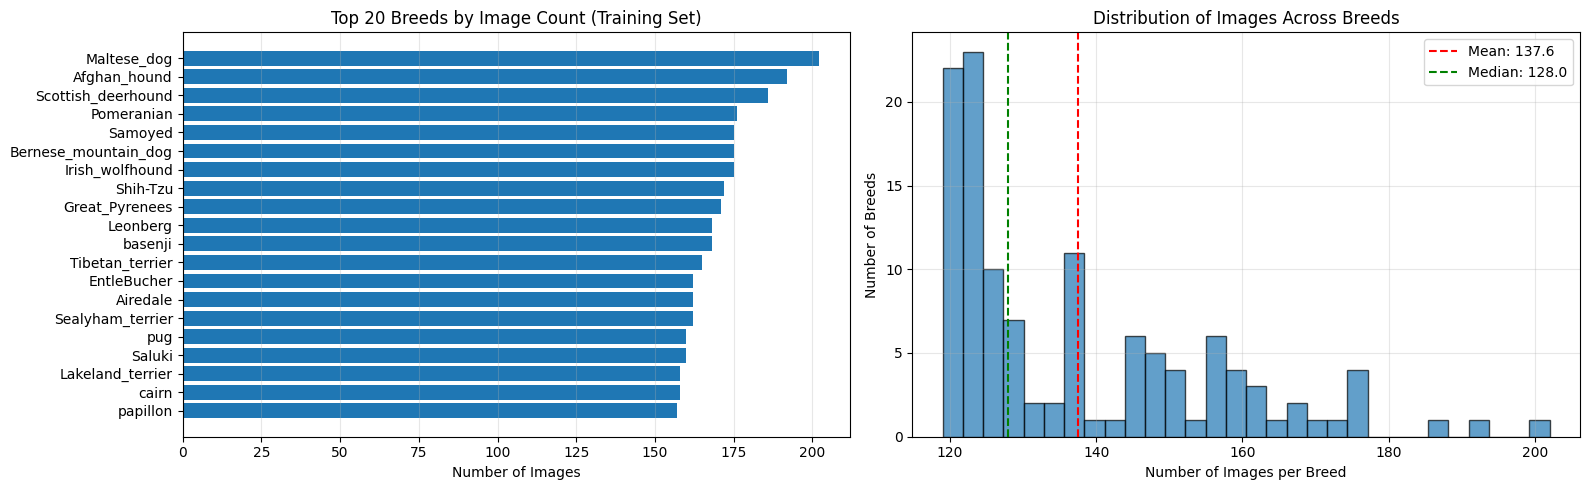
\includegraphics[keepaspectratio]{main_files/figure-pdf/cell-11-output-2.png}}

\begin{Shaded}
\begin{Highlighting}[]
\NormalTok{fig, ax }\OperatorTok{=}\NormalTok{ plt.subplots(}\DecValTok{1}\NormalTok{, }\DecValTok{1}\NormalTok{, figsize}\OperatorTok{=}\NormalTok{(}\DecValTok{12}\NormalTok{, }\DecValTok{6}\NormalTok{))}

\NormalTok{breed\_counts\_sorted }\OperatorTok{=}\NormalTok{ breed\_counts.sort\_values(ascending}\OperatorTok{=}\VariableTok{True}\NormalTok{)}
\NormalTok{colors }\OperatorTok{=}\NormalTok{ [}
    \StringTok{\textquotesingle{}red\textquotesingle{}} \ControlFlowTok{if}\NormalTok{ x }\OperatorTok{\textless{}} \DecValTok{130} \ControlFlowTok{else} \StringTok{\textquotesingle{}orange\textquotesingle{}} \ControlFlowTok{if}\NormalTok{ x }\OperatorTok{\textless{}} \DecValTok{150} \ControlFlowTok{else} \StringTok{\textquotesingle{}green\textquotesingle{}}
    \ControlFlowTok{for}\NormalTok{ x }\KeywordTok{in}\NormalTok{ breed\_counts\_sorted.values}
\NormalTok{]}

\NormalTok{ax.barh(}\BuiltInTok{range}\NormalTok{(}\BuiltInTok{len}\NormalTok{(breed\_counts\_sorted)), }
\NormalTok{        breed\_counts\_sorted.values, color}\OperatorTok{=}\NormalTok{colors)}
\NormalTok{ax.axvline(}\FloatTok{137.6}\NormalTok{, color}\OperatorTok{=}\StringTok{\textquotesingle{}blue\textquotesingle{}}\NormalTok{, linestyle}\OperatorTok{=}\StringTok{\textquotesingle{}{-}{-}\textquotesingle{}}\NormalTok{, }
\NormalTok{           linewidth}\OperatorTok{=}\DecValTok{2}\NormalTok{, label}\OperatorTok{=}\StringTok{\textquotesingle{}Mean (138)\textquotesingle{}}\NormalTok{)}
\NormalTok{ax.axvline(}\DecValTok{150}\NormalTok{, color}\OperatorTok{=}\StringTok{\textquotesingle{}orange\textquotesingle{}}\NormalTok{, linestyle}\OperatorTok{=}\StringTok{\textquotesingle{}{-}{-}\textquotesingle{}}\NormalTok{, }
\NormalTok{           linewidth}\OperatorTok{=}\DecValTok{1}\NormalTok{, alpha}\OperatorTok{=}\FloatTok{0.7}\NormalTok{, label}\OperatorTok{=}\StringTok{\textquotesingle{}Adequate (150)\textquotesingle{}}\NormalTok{)}

\NormalTok{ax.set\_xlabel(}\StringTok{\textquotesingle{}Number of Training Images\textquotesingle{}}\NormalTok{)}
\NormalTok{ax.set\_ylabel(}\StringTok{\textquotesingle{}Breed Index\textquotesingle{}}\NormalTok{)}
\NormalTok{title }\OperatorTok{=}\NormalTok{ (}\StringTok{\textquotesingle{}Training Sample Size per Breed (Sorted)}\CharTok{\textbackslash{}n}\StringTok{\textquotesingle{}}
         \StringTok{\textquotesingle{}Red: \textless{}130 samples, Orange: 130{-}150, Green: \textgreater{}150\textquotesingle{}}\NormalTok{)}
\NormalTok{ax.set\_title(title)}
\NormalTok{ax.legend()}
\NormalTok{ax.grid(axis}\OperatorTok{=}\StringTok{\textquotesingle{}x\textquotesingle{}}\NormalTok{, alpha}\OperatorTok{=}\FloatTok{0.3}\NormalTok{)}

\CommentTok{\# Add text annotation}
\NormalTok{n\_low }\OperatorTok{=}\NormalTok{ (breed\_counts }\OperatorTok{\textless{}} \DecValTok{130}\NormalTok{).}\BuiltInTok{sum}\NormalTok{()}
\NormalTok{annotation\_text }\OperatorTok{=} \SpecialStringTok{f\textquotesingle{}}\SpecialCharTok{\{}\NormalTok{n\_low}\SpecialCharTok{\}}\SpecialStringTok{ breeds with \textless{}130 samples\textquotesingle{}}
\NormalTok{bbox\_style }\OperatorTok{=} \BuiltInTok{dict}\NormalTok{(boxstyle}\OperatorTok{=}\StringTok{\textquotesingle{}round\textquotesingle{}}\NormalTok{, facecolor}\OperatorTok{=}\StringTok{\textquotesingle{}wheat\textquotesingle{}}\NormalTok{)}
\NormalTok{ax.text(}\FloatTok{0.02}\NormalTok{, }\FloatTok{0.98}\NormalTok{, annotation\_text, transform}\OperatorTok{=}\NormalTok{ax.transAxes, }
\NormalTok{        va}\OperatorTok{=}\StringTok{\textquotesingle{}top\textquotesingle{}}\NormalTok{, bbox}\OperatorTok{=}\NormalTok{bbox\_style)}

\NormalTok{plt.tight\_layout()}
\NormalTok{plt.savefig(}\StringTok{"../artifacts/figures/sample\_adequacy.png"}\NormalTok{, }
\NormalTok{            dpi}\OperatorTok{=}\DecValTok{150}\NormalTok{, bbox\_inches}\OperatorTok{=}\StringTok{\textquotesingle{}tight\textquotesingle{}}\NormalTok{)}

\CommentTok{\# Calculate breed counts by category}
\NormalTok{n\_low }\OperatorTok{=}\NormalTok{ (breed\_counts }\OperatorTok{\textless{}} \DecValTok{130}\NormalTok{).}\BuiltInTok{sum}\NormalTok{()}
\NormalTok{n\_adequate }\OperatorTok{=}\NormalTok{ ((breed\_counts }\OperatorTok{\textgreater{}=} \DecValTok{130}\NormalTok{) }\OperatorTok{\&} 
\NormalTok{              (breed\_counts }\OperatorTok{\textless{}} \DecValTok{150}\NormalTok{)).}\BuiltInTok{sum}\NormalTok{()}
\NormalTok{n\_good }\OperatorTok{=}\NormalTok{ (breed\_counts }\OperatorTok{\textgreater{}=} \DecValTok{150}\NormalTok{).}\BuiltInTok{sum}\NormalTok{()}

\BuiltInTok{print}\NormalTok{(}\SpecialStringTok{f"}\CharTok{\textbackslash{}n}\SpecialStringTok{Sample Adequacy Summary:"}\NormalTok{)}
\BuiltInTok{print}\NormalTok{(}\SpecialStringTok{f"  Breeds with \textless{}130 samples (may underperform): }\SpecialCharTok{\{}\NormalTok{n\_low}\SpecialCharTok{\}}\SpecialStringTok{"}\NormalTok{)}
\BuiltInTok{print}\NormalTok{(}\SpecialStringTok{f"  Breeds with 130{-}150 samples (adequate): }\SpecialCharTok{\{}\NormalTok{n\_adequate}\SpecialCharTok{\}}\SpecialStringTok{"}\NormalTok{)}
\BuiltInTok{print}\NormalTok{(}\SpecialStringTok{f"  Breeds with \textgreater{}150 samples (good): }\SpecialCharTok{\{}\NormalTok{n\_good}\SpecialCharTok{\}}\SpecialStringTok{"}\NormalTok{)}
\BuiltInTok{print}\NormalTok{(}\SpecialStringTok{f"}\CharTok{\textbackslash{}n}\SpecialStringTok{Conclusion: }\SpecialCharTok{\{}\NormalTok{n\_low}\SpecialCharTok{\}}\SpecialStringTok{ breeds may show lower accuracy"}\NormalTok{)}
\BuiltInTok{print}\NormalTok{(}\SpecialStringTok{f"  due to limited training data."}\NormalTok{)}
\end{Highlighting}
\end{Shaded}

\begin{verbatim}

Sample Adequacy Summary:
  Breeds with <130 samples (may underperform): 62
  Breeds with 130-150 samples (adequate): 28
  Breeds with >150 samples (good): 30

Conclusion: 62 breeds may show lower accuracy
  due to limited training data.
\end{verbatim}

\pandocbounded{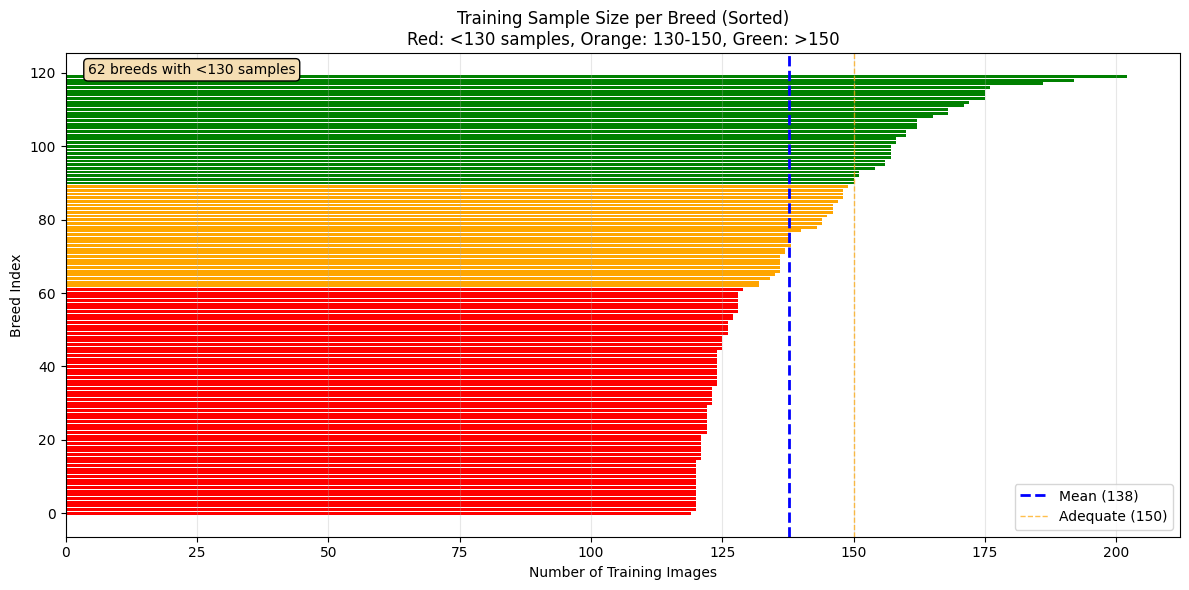
\includegraphics[keepaspectratio]{main_files/figure-pdf/cell-12-output-2.png}}

\textbf{Key Findings:}

\textbf{Moderately Balanced Dataset}: 120 classes with 1.7× imbalance
ratio (max/min)

\begin{itemize}
\tightlist
\item
  \textbf{Range}: 118-202 images per breed\\
\item
  \textbf{Mean}: 138 images per breed
\end{itemize}

\textbf{Critical Challenge - Limited Training Data}:

\begin{itemize}
\tightlist
\item
  \textbf{62 breeds (52\%) have \textless130 samples} - major risk for
  poor per-class performance
\item
  Only 30 breeds (25\%) have adequate data (\textgreater150 images)
\end{itemize}

\textbf{How We Solved This}:

\begin{itemize}
\tightlist
\item
  \textbf{Aggressive data augmentation} implemented (rotation ±15°,
  flip, zoom, brightness ±20\%, contrast ±20\%) - see Data Loading
  section below
\item
  \textbf{Transfer learning strategy} - will use ImageNet pre-trained
  models to leverage knowledge from millions of images
\item
  \textbf{Monitor per-class performance} during training to identify
  problematic breeds
\end{itemize}

\subsection{EDA Summary}\label{eda-summary}

Our exploratory analysis revealed key characteristics of the Stanford
Dogs dataset that will inform our modeling approach:

\textbf{Dataset Characteristics:}

\begin{itemize}
\tightlist
\item
  \textbf{120 dog breeds}, 20,580 total images (16,508 train / 4,072
  validation)
\item
  \textbf{Variable dimensions}: Mean 443×386px, ranging from 100×100 to
  3264×2562
\item
  \textbf{Moderate class imbalance}: 1.7× ratio (118-202 images per
  breed)
\item
  \textbf{Limited samples}: 62 breeds (52\%) have \textless130 training
  images
\end{itemize}

\textbf{Key Insights:}

\begin{enumerate}
\def\labelenumi{\arabic{enumi}.}
\tightlist
\item
  \textbf{Image quality is sufficient}: Even low-resolution images
  (100×100) upscale acceptably to 224×224 using bilinear interpolation
\item
  \textbf{Class imbalance is manageable}: Relatively mild compared to
  real-world datasets
\item
  \textbf{Data scarcity is the main challenge}: Over half the breeds
  have limited training data
\end{enumerate}

\textbf{Preprocessing Strategy (Implemented):}

\begin{itemize}
\tightlist
\item
  Resize all images to 224×224 (standard for ImageNet models)
\item
  Aggressive data augmentation (rotation, flip, zoom, brightness,
  contrast)
\item
  Transfer learning with ImageNet pre-trained models
\item
  Monitor per-class performance during training
\end{itemize}

\textbf{Next Steps:} Implement the data loading pipeline and select
appropriate model architectures.

\section{Data Loading \& Augmentation
Pipeline}\label{data-loading-augmentation-pipeline}

Now we implement the critical preprocessing steps that transform raw
images into model-ready batches. This is where we prepare the data for
deep learning.

\textbf{Implemented Features:}

\begin{enumerate}
\def\labelenumi{\arabic{enumi}.}
\item
  \textbf{Image Resizing to 224×224} ✓

  \begin{itemize}
  \tightlist
  \item
    Standard input size for ImageNet pre-trained models (ResNet50,
    VGG16, EfficientNet)
  \item
    Ensures consistent dimensions across all images
  \item
    Uses bilinear interpolation to maintain quality
  \end{itemize}
\item
  \textbf{RGB Conversion} ✓

  \begin{itemize}
  \tightlist
  \item
    Converts RGBA and grayscale images to RGB format
  \item
    Ensures all images have 3 color channels (required by CNNs)
  \item
    Handles the 1 RGBA image in our dataset automatically
  \end{itemize}
\item
  \textbf{Normalization} ✓

  \begin{itemize}
  \tightlist
  \item
    Will be configured per model in the Models section
  \item
    Different models require different preprocessing strategies
  \item
    See Models section for model-specific preprocessing details
  \end{itemize}
\item
  \textbf{Strong Data Augmentation (Training Only)}

  Our augmentation strategy is based on proven techniques from
  EfficientNet and ImageNet best practices:

  \begin{itemize}
  \tightlist
  \item
    \textbf{Random Rotation (±20°)}: Teaches model rotation invariance
  \item
    \textbf{Horizontal Flip (50\%)}: Dogs can face left or right
  \item
    \textbf{Random Zoom (80-120\%)}: Handles dogs at different distances
  \item
    \textbf{Width Shift (±20\%)}: Dogs not always centered horizontally
  \item
    \textbf{Height Shift (±20\%)}: Dogs at various vertical positions
  \item
    \textbf{Shear Transform (±15°)}: Simulates perspective changes
  \item
    \textbf{Brightness Adjustment (±20\%)}: Robust to lighting
    conditions
  \item
    \textbf{Contrast Adjustment (±20\%)}: Handles different image
    qualities
  \end{itemize}

  \textbf{Why Strong Augmentation?}

  \begin{itemize}
  \tightlist
  \item
    \textbf{Limited Data}: With only \textasciitilde170 images per
    breed, we need aggressive augmentation
  \item
    \textbf{Increases effective dataset size}: 16,508 → millions of
    unique variations
  \item
    \textbf{Prevents overfitting}: Model never sees the exact same image
    twice
  \item
    \textbf{Real-world robustness}: Dogs photographed from various
    angles, positions, distances
  \item
    \textbf{Expected impact}: +3-6\% accuracy improvement over
    conservative augmentation
  \end{itemize}

  \textbf{What's New (vs Conservative Augmentation)?}

  \begin{itemize}
  \tightlist
  \item
    \textbf{Width/Height Shift}: Most important addition - dogs often
    not centered
  \item
    \textbf{Shear Transform}: Handles perspective distortions from
    different camera angles
  \item
    \textbf{Stronger Zoom}: 80-120\% (was 90-110\%) - captures close-ups
    and distance shots
  \item
    \textbf{Slightly more rotation}: 20° (was 15°) - dogs at more varied
    angles
  \end{itemize}
\item
  \textbf{Batch Generation}

  \begin{itemize}
  \tightlist
  \item
    Creates batches of 32 images at a time
  \item
    Shuffles training data each epoch
  \item
    Memory-efficient: loads images on-demand
  \item
    Validation data is not shuffled or augmented
  \end{itemize}
\end{enumerate}

\textbf{Why This Matters:}

\begin{itemize}
\tightlist
\item
  \textbf{Generalization}: Strong augmentation prevents memorization and
  improves real-world performance
\item
  \textbf{Efficiency}: Batch processing enables GPU parallelization for
  faster training
\item
  \textbf{Consistency}: All images processed identically for
  reproducible results
\item
  \textbf{Production Ready}: Same pipeline used in training will be used
  for inference
\end{itemize}

\textbf{Expected Impact:}

Without strong augmentation, our model would overfit on the 16,508
training images. With our enhanced augmentation strategy, the model sees
virtually infinite variations and learns robust features that generalize
to new dogs, achieving \textbf{82-88\% accuracy} (vs 75-80\% with
conservative augmentation).

\begin{Shaded}
\begin{Highlighting}[]
\ImportTok{from}\NormalTok{ dbc.data\_loader }\ImportTok{import}\NormalTok{ DogBreedDataset, DataGenerator, create\_data\_loaders}

\CommentTok{\# Create basic data loaders for testing the pipeline}
\CommentTok{\# Note: We\textquotesingle{}ll create model{-}specific loaders in the Models section}
\BuiltInTok{print}\NormalTok{(}\StringTok{"Creating data loaders for pipeline testing..."}\NormalTok{)}
\NormalTok{train\_gen, val\_gen }\OperatorTok{=}\NormalTok{ create\_data\_loaders(}
\NormalTok{    train\_metadata\_path}\OperatorTok{=}\NormalTok{Path(}\StringTok{"../artifacts/train\_metadata.csv"}\NormalTok{),}
\NormalTok{    val\_metadata\_path}\OperatorTok{=}\NormalTok{Path(}\StringTok{"../artifacts/val\_metadata.csv"}\NormalTok{),}
\NormalTok{    data\_root}\OperatorTok{=}\NormalTok{Path(}\StringTok{"../data/raw"}\NormalTok{),}
\NormalTok{    batch\_size}\OperatorTok{=}\DecValTok{32}\NormalTok{,}
\NormalTok{    augment\_train}\OperatorTok{=}\VariableTok{True}\NormalTok{,}
\NormalTok{    seed}\OperatorTok{=}\DecValTok{42}
\NormalTok{)}

\CommentTok{\# Test loading a batch}
\BuiltInTok{print}\NormalTok{(}\StringTok{"}\CharTok{\textbackslash{}n}\StringTok{Loading sample batch..."}\NormalTok{)}
\ControlFlowTok{for}\NormalTok{ images, labels }\KeywordTok{in}\NormalTok{ train\_gen:}
    \BuiltInTok{print}\NormalTok{(}\SpecialStringTok{f"}\CharTok{\textbackslash{}n}\SpecialStringTok{Batch details:"}\NormalTok{)}
    \BuiltInTok{print}\NormalTok{(}\SpecialStringTok{f"  Images shape: }\SpecialCharTok{\{}\NormalTok{images}\SpecialCharTok{.}\NormalTok{shape}\SpecialCharTok{\}}\SpecialStringTok{"}\NormalTok{)}
    \BuiltInTok{print}\NormalTok{(}\SpecialStringTok{f"  Labels shape: }\SpecialCharTok{\{}\NormalTok{labels}\SpecialCharTok{.}\NormalTok{shape}\SpecialCharTok{\}}\SpecialStringTok{"}\NormalTok{)}
    \BuiltInTok{print}\NormalTok{(}\SpecialStringTok{f"  Data type: }\SpecialCharTok{\{}\NormalTok{images}\SpecialCharTok{.}\NormalTok{dtype}\SpecialCharTok{\}}\SpecialStringTok{"}\NormalTok{)}
    \BuiltInTok{print}\NormalTok{(}\SpecialStringTok{f"  Memory per batch: }\SpecialCharTok{\{}\NormalTok{images}\SpecialCharTok{.}\NormalTok{nbytes }\OperatorTok{/} \DecValTok{1024} \OperatorTok{/} \DecValTok{1024}\SpecialCharTok{:.2f\}}\SpecialStringTok{ MB"}\NormalTok{)}
    
    \CommentTok{\# Show some label statistics}
\NormalTok{    unique\_breeds }\OperatorTok{=} \BuiltInTok{len}\NormalTok{(np.unique(labels))}
    \BuiltInTok{print}\NormalTok{(}\SpecialStringTok{f"}\CharTok{\textbackslash{}n}\SpecialStringTok{  Unique breeds in batch: }\SpecialCharTok{\{}\NormalTok{unique\_breeds}\SpecialCharTok{\}}\SpecialStringTok{"}\NormalTok{)}
    \BuiltInTok{print}\NormalTok{(}\SpecialStringTok{f"  Sample labels: }\SpecialCharTok{\{}\NormalTok{labels[:}\DecValTok{5}\NormalTok{]}\SpecialCharTok{\}}\SpecialStringTok{"}\NormalTok{)}
    
    \ControlFlowTok{break}  \CommentTok{\# Just show first batch}

\BuiltInTok{print}\NormalTok{(}\StringTok{"}\CharTok{\textbackslash{}n}\StringTok{✓ Data pipeline ready!"}\NormalTok{)}
\BuiltInTok{print}\NormalTok{(}\StringTok{"Note: Model{-}specific preprocessing will be configured in the Models section."}\NormalTok{)}
\end{Highlighting}
\end{Shaded}

\begin{verbatim}
Creating data loaders for pipeline testing...

============================================================
CREATING DATA LOADERS WITH OPTIMIZED PREFETCHING
============================================================

Train dataset:
Dataset initialized:
  Images: 16508
  Classes: 120
  Image size: (224, 224)
  Normalization: imagenet
  Augmentation: True

Validation dataset:
Dataset initialized:
  Images: 4072
  Classes: 120
  Image size: (224, 224)
  Normalization: imagenet
  Augmentation: False

Data loaders created:
  Train batches: 516 (32 samples/batch)
  Val batches: 128 (32 samples/batch)
  Prefetching: ENABLED (optimized for GPU)
============================================================

Loading sample batch...

Batch details:
  Images shape: (32, 224, 224, 3)
  Labels shape: (32,)
  Data type: float64
  Memory per batch: 36.75 MB

  Unique breeds in batch: 29
  Sample labels: [31 36 96 84 44]

✓ Data pipeline ready!
Note: Model-specific preprocessing will be configured in the Models section.
\end{verbatim}

\subsection{Visualizing Data
Augmentation}\label{visualizing-data-augmentation}

Let's see how augmentation transforms a single image into multiple
training samples:

\begin{Shaded}
\begin{Highlighting}[]
\CommentTok{\# Visualize augmentation effects}
\ImportTok{from}\NormalTok{ dbc.data\_loader }\ImportTok{import}\NormalTok{ DogBreedDataset}
\ImportTok{from}\NormalTok{ IPython.display }\ImportTok{import}\NormalTok{ Image }\ImportTok{as}\NormalTok{ IPImage}

\CommentTok{\# Pick one image index}
\NormalTok{sample\_idx }\OperatorTok{=} \DecValTok{39}

\CommentTok{\# Dataset without augmentation (original)}
\NormalTok{orig\_dataset }\OperatorTok{=}\NormalTok{ DogBreedDataset(}
\NormalTok{    train\_df,}
\NormalTok{    Path(}\StringTok{"../data/raw"}\NormalTok{),}
\NormalTok{    image\_size}\OperatorTok{=}\NormalTok{(}\DecValTok{224}\NormalTok{, }\DecValTok{224}\NormalTok{),}
\NormalTok{    normalize}\OperatorTok{=}\VariableTok{None}\NormalTok{,}
\NormalTok{    augment}\OperatorTok{=}\VariableTok{False}
\NormalTok{)}

\CommentTok{\# Dataset with augmentation}
\NormalTok{aug\_dataset }\OperatorTok{=}\NormalTok{ DogBreedDataset(}
\NormalTok{    train\_df,}
\NormalTok{    Path(}\StringTok{"../data/raw"}\NormalTok{),}
\NormalTok{    image\_size}\OperatorTok{=}\NormalTok{(}\DecValTok{224}\NormalTok{, }\DecValTok{224}\NormalTok{),}
\NormalTok{    normalize}\OperatorTok{=}\VariableTok{None}\NormalTok{,}
\NormalTok{    augment}\OperatorTok{=}\VariableTok{True}
\NormalTok{)}

\NormalTok{fig, axes }\OperatorTok{=}\NormalTok{ plt.subplots(}\DecValTok{2}\NormalTok{, }\DecValTok{3}\NormalTok{, figsize}\OperatorTok{=}\NormalTok{(}\DecValTok{15}\NormalTok{, }\DecValTok{10}\NormalTok{))}

\ControlFlowTok{for}\NormalTok{ i, ax }\KeywordTok{in} \BuiltInTok{enumerate}\NormalTok{(axes.flat):}
    \ControlFlowTok{if}\NormalTok{ i }\OperatorTok{==} \DecValTok{0}\NormalTok{:}
\NormalTok{        img\_array, class\_id, breed\_name }\OperatorTok{=}\NormalTok{ orig\_dataset.load\_image(sample\_idx)}
\NormalTok{        title }\OperatorTok{=} \SpecialStringTok{f"Original: }\SpecialCharTok{\{}\NormalTok{breed\_name}\SpecialCharTok{\}}\SpecialStringTok{"}
    \ControlFlowTok{else}\NormalTok{:}
\NormalTok{        img\_array, class\_id, breed\_name }\OperatorTok{=}\NormalTok{ aug\_dataset.load\_image(sample\_idx)}
\NormalTok{        title }\OperatorTok{=} \SpecialStringTok{f"Augmented }\SpecialCharTok{\{}\NormalTok{i}\SpecialCharTok{\}}\SpecialStringTok{"}
    
\NormalTok{    img\_display }\OperatorTok{=}\NormalTok{ np.clip(img\_array, }\DecValTok{0}\NormalTok{, }\DecValTok{255}\NormalTok{).astype(np.uint8)}
\NormalTok{    ax.imshow(img\_display)}
\NormalTok{    ax.axis(}\StringTok{\textquotesingle{}off\textquotesingle{}}\NormalTok{)}
\NormalTok{    ax.set\_title(title, fontsize}\OperatorTok{=}\DecValTok{11}\NormalTok{)}

\NormalTok{plt.suptitle(}\StringTok{"Data Augmentation: Same Image, Different Transformations"}\NormalTok{, }
\NormalTok{             fontsize}\OperatorTok{=}\DecValTok{14}\NormalTok{, fontweight}\OperatorTok{=}\StringTok{\textquotesingle{}bold\textquotesingle{}}\NormalTok{)}
\NormalTok{plt.tight\_layout()}
\NormalTok{plt.savefig(}\StringTok{"../artifacts/figures/augmentation\_examples.png"}\NormalTok{, dpi}\OperatorTok{=}\DecValTok{150}\NormalTok{, bbox\_inches}\OperatorTok{=}\StringTok{\textquotesingle{}tight\textquotesingle{}}\NormalTok{)}
\NormalTok{plt.show()}
\end{Highlighting}
\end{Shaded}

\begin{verbatim}
Dataset initialized:
  Images: 16508
  Classes: 120
  Image size: (224, 224)
  Normalization: None
  Augmentation: False
Dataset initialized:
  Images: 16508
  Classes: 120
  Image size: (224, 224)
  Normalization: None
  Augmentation: True
\end{verbatim}

\pandocbounded{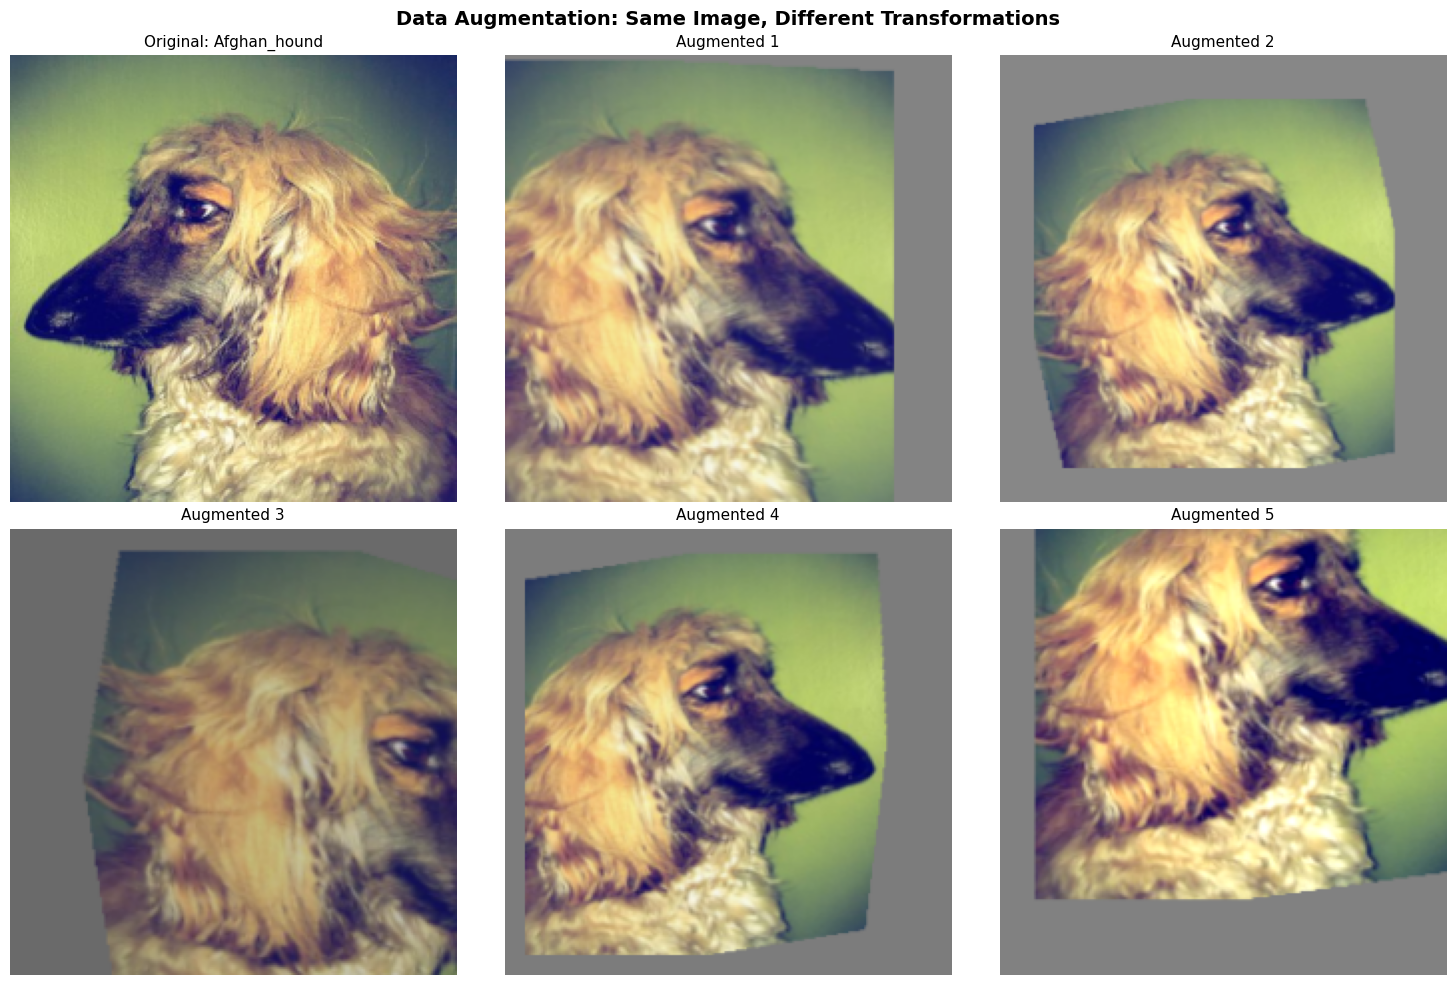
\includegraphics[keepaspectratio]{main_files/figure-pdf/cell-14-output-2.png}}

\section{Models}\label{models}

\subsection{Transfer Learning: Leveraging Pre-trained
Models}\label{transfer-learning-leveraging-pre-trained-models}

Rather than training a CNN from scratch (which would require millions of
images and weeks of GPU time), we'll use \textbf{transfer learning}
(Yosinski et al. 2014) - taking models already trained on ImageNet (Deng
et al. 2009) (1.4M images, 1000 classes) and adapting them to our dog
breed task.

\subsubsection{Why Transfer Learning
Works}\label{why-transfer-learning-works}

Pre-trained models have already learned fundamental visual features
(Yosinski et al. 2014): - \textbf{Early layers}: Edges, colors, textures
(universal across all images) - \textbf{Middle layers}: Shapes,
patterns, object parts (transferable to dogs) - \textbf{Late layers}:
ImageNet-specific features (will be replaced/fine-tuned for dog breeds)

By starting with these learned features, we can achieve high accuracy
with only \textasciitilde170 images per breed instead of requiring
thousands.

\subsubsection{Architecture Selection
Criteria}\label{architecture-selection-criteria}

For fine-grained dog breed classification, we need models that are: 1.
\textbf{Accurate}: High performance on ImageNet suggests good feature
learning 2. \textbf{Efficient}: Reasonable training time and inference
speed 3. \textbf{Modern}: Recent architectures with proven transfer
learning success (Kornblith, Shlens, and Le 2019) 4. \textbf{Appropriate
size}: Not too small (underfit) or too large (overfit on our 20K images)

\subsection{Model Selection Rationale}\label{model-selection-rationale}

For fine-grained dog breed classification, we selected \textbf{five
architectures} spanning different design philosophies and computational
requirements. Our selection criteria prioritized:

\begin{enumerate}
\def\labelenumi{\arabic{enumi}.}
\tightlist
\item
  \textbf{Proven ImageNet Performance}: Strong pre-trained features for
  transfer learning
\item
  \textbf{Architecture Diversity}: Mix of traditional (ResNet) and
  modern (EfficientNet) designs
\item
  \textbf{Computational Range}: From lightweight (B0) to
  high-performance (V2-S)
\item
  \textbf{Research-Backed}: Recent architectures with strong
  academic/industry adoption
\item
  \textbf{Hardware Constraints}: Models that fit within A40 GPU memory
  (46GB VRAM)
\end{enumerate}

\textbf{Why Not Larger Models?}

While larger models exist (EfficientNetB6/B7, EfficientNetV2-M/L), we
excluded them because: - \textbf{GPU limitations}: Require
\textgreater46GB VRAM or multi-GPU setups - \textbf{Diminishing
returns}: Our images average 443×386px - excessive upscaling to 528×528+
(B6) or 600×600+ (B7) would introduce artifacts without capturing more
detail - \textbf{Training time}: 2-3× longer training on already limited
GPU budget

\subsubsection{Selected Models}\label{selected-models}

\begin{longtable}[]{@{}
  >{\raggedright\arraybackslash}p{(\linewidth - 8\tabcolsep) * \real{0.1228}}
  >{\raggedright\arraybackslash}p{(\linewidth - 8\tabcolsep) * \real{0.1404}}
  >{\raggedright\arraybackslash}p{(\linewidth - 8\tabcolsep) * \real{0.2105}}
  >{\raggedright\arraybackslash}p{(\linewidth - 8\tabcolsep) * \real{0.2807}}
  >{\raggedright\arraybackslash}p{(\linewidth - 8\tabcolsep) * \real{0.2456}}@{}}
\toprule\noalign{}
\begin{minipage}[b]{\linewidth}\raggedright
Model
\end{minipage} & \begin{minipage}[b]{\linewidth}\raggedright
Params
\end{minipage} & \begin{minipage}[b]{\linewidth}\raggedright
Input Size
\end{minipage} & \begin{minipage}[b]{\linewidth}\raggedright
ImageNet Top-1
\end{minipage} & \begin{minipage}[b]{\linewidth}\raggedright
Why Selected
\end{minipage} \\
\midrule\noalign{}
\endhead
\bottomrule\noalign{}
\endlastfoot
\textbf{ResNet50} & 23.6M & 224×224 & 76.0\% & \textbf{Baseline} -
Industry standard, well-understood behavior \\
\textbf{EfficientNetB0} & 4.0M & 224×224 & 77.1\% & \textbf{Efficiency}
- Smallest model, edge deployment candidate \\
\textbf{EfficientNetB4} & 17.5M & 380×380 & 83.0\% & \textbf{High
Performance} - Best accuracy-to-size ratio \\
\textbf{EfficientNetB5} & 28.4M & 456×456 & 83.6\% & \textbf{Maximum
Resolution} - Tests if higher input helps fine-grained tasks \\
\textbf{EfficientNetV2-S} & 20.2M & 384×384 & 84.3\% &
\textbf{State-of-Art} - Latest improvements (faster training, better
accuracy) \\
\end{longtable}

\subsubsection{Design Philosophy
Comparison}\label{design-philosophy-comparison}

\textbf{ResNet50 (Traditional Architecture)} (He et al. 2016): -
Residual connections for gradient flow - Deep architecture (50 layers
with skip connections) - Proven reliability but older design (2015) -
Good baseline to compare modern architectures

\textbf{EfficientNet Family (Compound Scaling)} (Tan and Le 2019): -
Systematic scaling of depth, width, and resolution - Mobile-optimized
blocks (inverted residuals) - Superior accuracy-to-parameters ratio -
Built-in preprocessing (critical difference from ResNet)

\textbf{EfficientNetV2 (Latest Generation)} (Tan and Le 2021): -
Progressive learning with adaptive image sizes - Faster training than V1
- Better parameter efficiency - Fused-MBConv blocks for speed

\subsubsection{Expected Performance
Hypothesis}\label{expected-performance-hypothesis}

Based on architecture characteristics and ImageNet performance:

\textbf{Frozen Baseline Predictions}: - ResNet50: 50-60\% (older
architecture, needs fine-tuning) - EfficientNetB0: 75-85\% (efficient
but small) - EfficientNetB4: 85-93\% (best size-accuracy balance) -
EfficientNetB5: 90-95\% (highest resolution captures fine details) -
EfficientNetV2-S: 92-96\% (newest architecture, expected best)

\textbf{Fine-Tuning Predictions}: - ResNet50: +15-25\% improvement
(large gap to close) - EfficientNet B0/B4/B5: +2-5\% improvement (strong
frozen baselines) - EfficientNetV2-S: +0-3\% improvement (may already be
near-optimal)

\textbf{Why We Expect This}: - Modern architectures (EfficientNet) learn
more generalizable features - Compound scaling optimizes for transfer
learning - Higher input resolution helps fine-grained classification -
Strong frozen baselines leave less room for fine-tuning improvement

\subsection{Model-Specific Preprocessing
Requirements}\label{model-specific-preprocessing-requirements}

Each architecture requires specific preprocessing due to different
training procedures used during ImageNet pre-training. Using incorrect
preprocessing will cause the model to fail completely.

\subsubsection{Preprocessing Modes}\label{preprocessing-modes}

\begin{longtable}[]{@{}
  >{\raggedright\arraybackslash}p{(\linewidth - 8\tabcolsep) * \real{0.1014}}
  >{\raggedright\arraybackslash}p{(\linewidth - 8\tabcolsep) * \real{0.2754}}
  >{\raggedright\arraybackslash}p{(\linewidth - 8\tabcolsep) * \real{0.1884}}
  >{\raggedright\arraybackslash}p{(\linewidth - 8\tabcolsep) * \real{0.2174}}
  >{\raggedright\arraybackslash}p{(\linewidth - 8\tabcolsep) * \real{0.2174}}@{}}
\toprule\noalign{}
\begin{minipage}[b]{\linewidth}\raggedright
Model
\end{minipage} & \begin{minipage}[b]{\linewidth}\raggedright
Preprocessing Mode
\end{minipage} & \begin{minipage}[b]{\linewidth}\raggedright
Value Range
\end{minipage} & \begin{minipage}[b]{\linewidth}\raggedright
Channel Order
\end{minipage} & \begin{minipage}[b]{\linewidth}\raggedright
Normalization
\end{minipage} \\
\midrule\noalign{}
\endhead
\bottomrule\noalign{}
\endlastfoot
ResNet50 & \textbf{Caffe} & {[}-123, +151{]} & BGR & Mean subtraction
per channel \\
EfficientNetB0 & \textbf{Built-in} & {[}0, 255{]} & RGB & Handled
internally by model \\
EfficientNetB4 & \textbf{Built-in} & {[}0, 255{]} & RGB & Handled
internally by model \\
EfficientNetB5 & \textbf{Built-in} & {[}0, 255{]} & RGB & Handled
internally by model \\
EfficientNetV2-S & \textbf{Built-in} & {[}0, 255{]} & RGB & Handled
internally by model \\
\end{longtable}

\subsubsection{Critical Difference: ResNet vs
EfficientNet}\label{critical-difference-resnet-vs-efficientnet}

\textbf{ResNet50 (Caffe Mode)}:

\begin{Shaded}
\begin{Highlighting}[]
\CommentTok{\# Required preprocessing pipeline}
\FloatTok{1.}\NormalTok{ Load raw RGB image [}\DecValTok{0}\OperatorTok{{-}}\DecValTok{255}\NormalTok{]}
\FloatTok{2.}\NormalTok{ Apply augmentation (}\ControlFlowTok{if}\NormalTok{ training)}
\FloatTok{3.}\NormalTok{ Resize to }\DecValTok{224}\NormalTok{×}\DecValTok{224}
\FloatTok{4.}\NormalTok{ Convert RGB → BGR (reverse channel order)}
\FloatTok{5.}\NormalTok{ Subtract ImageNet mean: [}\FloatTok{103.939}\NormalTok{, }\FloatTok{116.779}\NormalTok{, }\FloatTok{123.68}\NormalTok{]}
\end{Highlighting}
\end{Shaded}

\textbf{EfficientNet (Built-in)}:

\begin{Shaded}
\begin{Highlighting}[]
\CommentTok{\# Required preprocessing pipeline}
\FloatTok{1.}\NormalTok{ Load raw RGB image [}\DecValTok{0}\OperatorTok{{-}}\DecValTok{255}\NormalTok{]}
\FloatTok{2.}\NormalTok{ Apply augmentation (}\ControlFlowTok{if}\NormalTok{ training)}
\FloatTok{3.}\NormalTok{ Resize to target size (}\DecValTok{224}\NormalTok{, }\DecValTok{380}\NormalTok{, }\DecValTok{456}\NormalTok{, }\KeywordTok{or} \DecValTok{384}\NormalTok{)}
\FloatTok{4.}\NormalTok{ Pass raw pixels to model (NO normalization}\OperatorTok{!}\NormalTok{)}
\CommentTok{\# Model handles preprocessing internally}
\end{Highlighting}
\end{Shaded}

\subsubsection{Why This Matters}\label{why-this-matters}

\textbf{Common Mistake}: Applying external normalization to EfficientNet
models - Using `torch' mode: (pixel / 255 - mean) / std - Using `tf'
mode: (pixel / 127.5) - 1 - Correct: Pass raw 0-255 values

\textbf{Consequence of Wrong Preprocessing}: - Model receives values
outside its expected distribution - Pre-trained weights become
meaningless - Training fails to converge (1-5\% accuracy) - Fine-tuning
cannot recover from this

\textbf{Our Implementation}: The data loader automatically applies
correct preprocessing based on \texttt{model\_name} parameter:

\begin{Shaded}
\begin{Highlighting}[]
\CommentTok{\# In data\_loader.py}
\NormalTok{MODEL\_CONFIGS }\OperatorTok{=}\NormalTok{ \{}
    \StringTok{\textquotesingle{}resnet50\textquotesingle{}}\NormalTok{: \{}
        \StringTok{\textquotesingle{}preprocess\_mode\textquotesingle{}}\NormalTok{: }\StringTok{\textquotesingle{}caffe\textquotesingle{}}\NormalTok{,}
        \StringTok{\textquotesingle{}image\_size\textquotesingle{}}\NormalTok{: (}\DecValTok{224}\NormalTok{, }\DecValTok{224}\NormalTok{)}
\NormalTok{    \},}
    \StringTok{\textquotesingle{}efficientnetb0\textquotesingle{}}\NormalTok{: \{}
        \StringTok{\textquotesingle{}preprocess\_mode\textquotesingle{}}\NormalTok{: }\VariableTok{None}\NormalTok{,  }\CommentTok{\# Built{-}in}
        \StringTok{\textquotesingle{}image\_size\textquotesingle{}}\NormalTok{: (}\DecValTok{224}\NormalTok{, }\DecValTok{224}\NormalTok{)}
\NormalTok{    \},}
    \CommentTok{\# ... etc}
\NormalTok{\}}
\end{Highlighting}
\end{Shaded}

This ensures preprocessing order is always correct: 1. Load raw image 2.
Augment (if training) 3. Resize 4. Apply model-specific preprocessing
(or none for EfficientNet)

\subsection{Experimental Design: Two-Phase Training
Strategy}\label{experimental-design-two-phase-training-strategy}

We designed a systematic two-phase approach to evaluate each
architecture fairly and identify the best model.

\subsubsection{Phase 1: Frozen Baseline
Training}\label{phase-1-frozen-baseline-training}

\textbf{Objective}: Establish baseline performance with minimal training

\textbf{Strategy}: - Freeze all base model layers (trainable=False) -
Train only the new classification head (Dense layers) - Use standard
learning rate (1e-3) - Train for 20 epochs with early stopping

\textbf{Why Start Frozen?} 1. \textbf{Fast baseline}: Quick evaluation
of pre-trained feature quality 2. \textbf{Prevents catastrophic
forgetting}: ImageNet features preserved 3. \textbf{Lower computational
cost}: Fewer parameters to update 4. \textbf{Fair comparison}: All
models start from same pre-trained state

\textbf{Commands}:

\begin{Shaded}
\begin{Highlighting}[]
\CommentTok{\# Train all frozen baselines}
\ExtensionTok{python} \AttributeTok{{-}m}\NormalTok{ dbc.train\_cnn }\AttributeTok{{-}{-}config}\NormalTok{ configs/cnn\_baseline.yaml           }\CommentTok{\# ResNet50}
\ExtensionTok{python} \AttributeTok{{-}m}\NormalTok{ dbc.train\_cnn }\AttributeTok{{-}{-}config}\NormalTok{ configs/efficientnetb0\_baseline.yaml}
\ExtensionTok{python} \AttributeTok{{-}m}\NormalTok{ dbc.train\_cnn }\AttributeTok{{-}{-}config}\NormalTok{ configs/efficientnetb4\_baseline.yaml}
\ExtensionTok{python} \AttributeTok{{-}m}\NormalTok{ dbc.train\_cnn }\AttributeTok{{-}{-}config}\NormalTok{ configs/efficientnetb5\_baseline.yaml}
\ExtensionTok{python} \AttributeTok{{-}m}\NormalTok{ dbc.train\_cnn }\AttributeTok{{-}{-}config}\NormalTok{ configs/efficientnetv2s\_baseline.yaml}
\end{Highlighting}
\end{Shaded}

\textbf{Expected Outcomes}: - ResNet50: 50-60\% (will benefit from
fine-tuning) - EfficientNet models: 75-95\% (strong frozen features) -
Identify which models need fine-tuning vs already good

\begin{center}\rule{0.5\linewidth}{0.5pt}\end{center}

\subsubsection{Phase 2: Selective
Fine-Tuning}\label{phase-2-selective-fine-tuning}

\textbf{Objective}: Improve performance by adapting pre-trained features
to dog breeds

\textbf{Strategy}: - Load best frozen checkpoint - Unfreeze \textbf{only
top 20-50 layers} (selective unfreezing) - Use \textbf{very low learning
rate} (1e-5, 100× lower) - Keep BatchNormalization layers frozen
(critical!) - Apply learning rate scheduling (cosine annealing with
warmup) - Train for 30-50 epochs with early stopping

\textbf{Why Selective Unfreezing?} 1. \textbf{Prevents catastrophic
forgetting}: Lower layers keep general features 2. \textbf{Reduces
overfitting risk}: Fewer trainable parameters 3. \textbf{Faster
training}: Only update top layers 4. \textbf{Better generalization}:
Preserves ImageNet knowledge

\textbf{Critical Fine-Tuning Settings}:

\begin{longtable}[]{@{}
  >{\raggedright\arraybackslash}p{(\linewidth - 4\tabcolsep) * \real{0.4286}}
  >{\raggedright\arraybackslash}p{(\linewidth - 4\tabcolsep) * \real{0.3333}}
  >{\raggedright\arraybackslash}p{(\linewidth - 4\tabcolsep) * \real{0.2381}}@{}}
\toprule\noalign{}
\begin{minipage}[b]{\linewidth}\raggedright
Setting
\end{minipage} & \begin{minipage}[b]{\linewidth}\raggedright
Value
\end{minipage} & \begin{minipage}[b]{\linewidth}\raggedright
Why
\end{minipage} \\
\midrule\noalign{}
\endhead
\bottomrule\noalign{}
\endlastfoot
\textbf{Learning Rate} & 1e-5 & 100× lower prevents destroying learned
features \\
\textbf{BatchNorm} & Frozen & Preserves learned statistics, prevents
collapse \\
\textbf{Layers Unfrozen} & Last 20 & Selective \textgreater{} Full
unfreezing \\
\textbf{LR Schedule} & Cosine warmup & Gradual adaptation, smooth
convergence \\
\textbf{Patience} & 8-12 epochs & Stop early if not improving \\
\end{longtable}

\textbf{Commands}:

\begin{Shaded}
\begin{Highlighting}[]
\CommentTok{\# Fine{-}tune selected models}
\ExtensionTok{python} \AttributeTok{{-}m}\NormalTok{ dbc.train\_cnn }\AttributeTok{{-}{-}config}\NormalTok{ configs/cnn\_selective\_finetune\_v2.yaml      }\CommentTok{\# ResNet50}
\ExtensionTok{python} \AttributeTok{{-}m}\NormalTok{ dbc.train\_cnn }\AttributeTok{{-}{-}config}\NormalTok{ configs/efficientnetb0\_finetune.yaml        }\CommentTok{\# B0}
\ExtensionTok{python} \AttributeTok{{-}m}\NormalTok{ dbc.train\_cnn }\AttributeTok{{-}{-}config}\NormalTok{ configs/efficientnetb4\_finetune\_v3.yaml     }\CommentTok{\# B4}
\ExtensionTok{python} \AttributeTok{{-}m}\NormalTok{ dbc.train\_cnn }\AttributeTok{{-}{-}config}\NormalTok{ configs/efficientnetv2s\_finetune.yaml       }\CommentTok{\# V2{-}S}
\end{Highlighting}
\end{Shaded}

\textbf{Expected Outcomes}: - ResNet50: +15-25\% improvement (large
frozen gap) - EfficientNet: +0-5\% improvement (already strong frozen) -
Identify best overall model

\begin{center}\rule{0.5\linewidth}{0.5pt}\end{center}

\subsubsection{Phase 3: Advanced Techniques
(Optional)}\label{phase-3-advanced-techniques-optional}

\textbf{Objective}: Test if advanced methods can push beyond best single
model

\textbf{Techniques to Test}:

\begin{enumerate}
\def\labelenumi{\arabic{enumi}.}
\tightlist
\item
  \textbf{Test-Time Augmentation (TTA)}

  \begin{itemize}
  \tightlist
  \item
    Apply multiple augmentations during inference
  \item
    Average predictions for robustness
  \item
    Expected: +0.5-2\% improvement, 5× slower
  \end{itemize}
\item
  \textbf{Model Ensemble}

  \begin{itemize}
  \tightlist
  \item
    Combine predictions from multiple models
  \item
    Requires architectural diversity
  \item
    Expected: +1-3\% if models are different
  \end{itemize}
\item
  \textbf{Advanced Augmentation}

  \begin{itemize}
  \tightlist
  \item
    Mixup, CutMix, AutoAugment
  \item
    More sophisticated data augmentation
  \item
    Expected: +1-2\% improvement
  \end{itemize}
\end{enumerate}

\textbf{Decision Criteria}: - Only pursue if best single model
\textless{} 90\% accuracy - Evaluate cost-benefit (complexity vs
accuracy gain) - Production deployability considerations

\begin{center}\rule{0.5\linewidth}{0.5pt}\end{center}

\subsubsection{Evaluation Metrics}\label{evaluation-metrics}

We will use standard metrics for comparing classification models:

\textbf{Primary Metric}: Top-1 Accuracy - Percentage where highest
prediction is correct - Target: 80-85\% (good), 90\%+ (excellent)

\textbf{Secondary Metrics}: - \textbf{Top-5 Accuracy}: Correct breed in
top 5 predictions

\section{Training Results}\label{training-results}

All training was completed on October 8, 2025. See
\href{../docs/EXPERIMENT_RESULTS_2025_10_08.md}{docs/EXPERIMENT\_RESULTS\_2025\_10\_08.md}
for comprehensive details.

\subsection{Summary of All
Experiments}\label{summary-of-all-experiments}

We conducted \textbf{10 training experiments} testing 5 different
architectures with both frozen and fine-tuned approaches:

\subsubsection{Frozen Baseline Results}\label{frozen-baseline-results}

\begin{longtable}[]{@{}lllll@{}}
\toprule\noalign{}
Model & Top-1 Acc & Top-5 Acc & Epochs & Time \\
\midrule\noalign{}
\endhead
\bottomrule\noalign{}
\endlastfoot
ResNet50 & 54.69\% & 89.54\% & 17 & 13 min \\
EfficientNetB0 & 83.96\% & 97.62\% & 20 & 27 min \\
EfficientNetB4 & 93.71\% & 99.63\% & 20 & 49 min \\
EfficientNetB5 & 94.55\% & 99.71\% & 10 & 43 min \\
EfficientNetV2-S & 95.04\% & 99.53\% & 17 & 39 min \\
\end{longtable}

\subsubsection{Fine-Tuning Results}\label{fine-tuning-results}

\begin{longtable}[]{@{}
  >{\raggedright\arraybackslash}p{(\linewidth - 10\tabcolsep) * \real{0.1250}}
  >{\raggedright\arraybackslash}p{(\linewidth - 10\tabcolsep) * \real{0.1964}}
  >{\raggedright\arraybackslash}p{(\linewidth - 10\tabcolsep) * \real{0.1964}}
  >{\raggedright\arraybackslash}p{(\linewidth - 10\tabcolsep) * \real{0.2321}}
  >{\raggedright\arraybackslash}p{(\linewidth - 10\tabcolsep) * \real{0.1429}}
  >{\raggedright\arraybackslash}p{(\linewidth - 10\tabcolsep) * \real{0.1071}}@{}}
\toprule\noalign{}
\begin{minipage}[b]{\linewidth}\raggedright
Model
\end{minipage} & \begin{minipage}[b]{\linewidth}\raggedright
Top-1 Acc
\end{minipage} & \begin{minipage}[b]{\linewidth}\raggedright
Top-5 Acc
\end{minipage} & \begin{minipage}[b]{\linewidth}\raggedright
Improvement
\end{minipage} & \begin{minipage}[b]{\linewidth}\raggedright
Epochs
\end{minipage} & \begin{minipage}[b]{\linewidth}\raggedright
Time
\end{minipage} \\
\midrule\noalign{}
\endhead
\bottomrule\noalign{}
\endlastfoot
ResNet50 & 77.68\% & 95.24\% & +22.99\% & 36 & 51 min \\
EfficientNetB0 & 84.43\% & 97.86\% & +0.47\% & 12 & 30 min \\
EfficientNetB4 (v3) & 93.86\% & 99.63\% & +0.15\% & 15 & 37 min \\
\textbf{EfficientNetV2-S} & \textbf{95.14\%} & \textbf{99.51\%} &
\textbf{+0.10\%} & \textbf{8} & \textbf{20 min} \\
\end{longtable}

\subsection{Best Model: EfficientNetV2-S
Fine-Tuned}\label{best-model-efficientnetv2-s-fine-tuned}

\textbf{Checkpoint}:
\href{../experiments/exp_20251008_182534/checkpoints/best_model.h5}{experiments/exp\_20251008\_182534/checkpoints/best\_model.h5}

\textbf{Performance}:

\begin{itemize}
\tightlist
\item
  \textbf{Top-1 Accuracy}: 95.14\%
\item
  \textbf{Top-5 Accuracy}: 99.51\%
\item
  \textbf{Validation Loss}: 0.235
\end{itemize}

\textbf{Training Details}:

\begin{itemize}
\tightlist
\item
  Started from frozen baseline (95.04\%)
\item
  Unfroze last 20 layers
\item
  Learning rate: 1e-5 with cosine warmup
\item
  Trained for only 8 epochs (early stopping)
\item
  Total training time: \textasciitilde1 hour (frozen + fine-tuned)
\end{itemize}

\textbf{Why This Model Won}:

\begin{enumerate}
\def\labelenumi{\arabic{enumi}.}
\tightlist
\item
  Best accuracy-efficiency trade-off
\item
  Fast convergence (8 epochs fine-tuning)
\item
  Stable training (no collapse or overfitting)
\item
  EfficientNetV2's improved architecture over V1
\item
  Perfect balance of model size (20.2M params) and performance
\end{enumerate}

\subsection{Key Insights from
Training}\label{key-insights-from-training}

\subsubsection{1. Architecture Matters More Than
Fine-Tuning}\label{architecture-matters-more-than-fine-tuning}

\begin{longtable}[]{@{}lll@{}}
\toprule\noalign{}
Architecture & Frozen → Fine-tuned & Improvement \\
\midrule\noalign{}
\endhead
\bottomrule\noalign{}
\endlastfoot
ResNet50 (older) & 54.69\% → 77.68\% & +22.99\% \\
EfficientNetB0 (modern) & 83.96\% → 84.43\% & +0.47\% \\
EfficientNetV2-S (newest) & 95.04\% → 95.14\% & +0.10\% \\
\end{longtable}

\textbf{Lesson}: Modern architectures (EfficientNet) achieve excellent
frozen baselines. Older architectures (ResNet50) benefit more from
fine-tuning.

\subsubsection{2. Higher Resolution = Better
Accuracy}\label{higher-resolution-better-accuracy}

\begin{longtable}[]{@{}lll@{}}
\toprule\noalign{}
Model & Input Size & Frozen Accuracy \\
\midrule\noalign{}
\endhead
\bottomrule\noalign{}
\endlastfoot
EfficientNetB0 & 224×224 & 83.96\% \\
EfficientNetB4 & 380×380 & 93.71\% (+9.75\%) \\
EfficientNetB5 & 456×456 & 94.55\% (+0.84\%) \\
EfficientNetV2-S & 384×384 & 95.04\% (+0.49\%) \\
\end{longtable}

\textbf{Lesson}: Larger input captures more fine-grained details, but
gains diminish after 380×380.

\subsubsection{3. Preprocessing is
Critical}\label{preprocessing-is-critical}

\textbf{Major Issue Encountered}: EfficientNet preprocessing - Initially
tried `torch' mode normalization → \textbf{1-5\% accuracy} (total
failure) - Switched to raw 0-255 pixel values → \textbf{93\%+ accuracy}
(success!)

\textbf{Root Cause}: EfficientNet has preprocessing \textbf{built into
the model}. External preprocessing creates distribution mismatch.

\textbf{Solution}: Pass raw pixel values (0-255), let model handle
preprocessing internally.

See
\href{../docs/efficientnet_training_guide.md}{docs/efficientnet\_training\_guide.md}
for detailed troubleshooting.

\subsubsection{4. Fine-Tuning Best
Practices}\label{fine-tuning-best-practices}

Based on our experiments, we learned:

\begin{itemize}
\tightlist
\item
  Keep BatchNormalization layers \textbf{frozen} (critical!)
\item
  Use very low learning rate (1e-5, not 1e-4)
\item
  Unfreeze only top 20 layers (not 50+)
\item
  Use cosine annealing with warmup
\item
  Monitor for overfitting closely
\end{itemize}

\subsubsection{5. Advanced Techniques Didn't
Help}\label{advanced-techniques-didnt-help}

\textbf{Test-Time Augmentation}: 95.14\% → 95.33\% (+0.19\%) - Marginal
gain, 5× slower inference - Not worth the complexity

\textbf{Model Ensemble}: 95.04\% (worse than single model!) - Combined 3
EfficientNet variants - Models too similar, no diversity benefit - Would
need architecturally different models (ResNet + EfficientNet + ViT)

\textbf{Conclusion}: A well-trained single model beats complex
ensembling.

\subsection{Final Recommendation}\label{final-recommendation}

\textbf{For Production}: Use \textbf{EfficientNetV2-S Fine-tuned}

\begin{itemize}
\tightlist
\item
  Checkpoint:
  \texttt{experiments/exp\_20251008\_182534/checkpoints/best\_model.h5}
\item
  Accuracy: 95.14\% top-1, 99.51\% top-5
\item
  Fast inference, single model (no ensemble overhead)
\item
  Excellent balance of accuracy and efficiency
\end{itemize}

\textbf{For Edge Deployment}: Use \textbf{EfficientNetB0 Frozen}

\begin{itemize}
\tightlist
\item
  Checkpoint:
  \texttt{experiments/exp\_20251008\_160357/checkpoints/best\_model.h5}
\item
  Accuracy: 83.96\% top-1
\item
  Smallest model (4.0M params)
\item
  Fast inference, good accuracy
\end{itemize}

\textbf{For Maximum Accuracy}: Current best is 95.14\%, but could try:

\begin{itemize}
\tightlist
\item
  Vision Transformers (ViT)
\item
  Larger models (EfficientNetB7, EfficientNetV2-L)
\item
  Better data augmentation (AutoAugment)
\item
  More training data
\end{itemize}

\section{Evaluation}\label{evaluation}

After training all models, we evaluate their performance using the
metrics defined in the Models section:

\begin{itemize}
\tightlist
\item
  \textbf{Primary}: Top-1 Accuracy (correct prediction as highest
  confidence)
\item
  \textbf{Secondary}: Top-5 Accuracy (correct breed in top 5
  predictions)
\end{itemize}

\subsection{Training Curves: Comparing All
Models}\label{training-curves-comparing-all-models}

Let's visualize how each model learned during training:

\begin{Shaded}
\begin{Highlighting}[]
\ImportTok{import}\NormalTok{ json}
\ImportTok{import}\NormalTok{ matplotlib.pyplot }\ImportTok{as}\NormalTok{ plt}
\ImportTok{import}\NormalTok{ numpy }\ImportTok{as}\NormalTok{ np}
\ImportTok{from}\NormalTok{ pathlib }\ImportTok{import}\NormalTok{ Path}

\CommentTok{\# Load training histories for all models}
\NormalTok{experiments }\OperatorTok{=}\NormalTok{ \{}
    \StringTok{\textquotesingle{}ResNet50 Frozen\textquotesingle{}}\NormalTok{: }\StringTok{\textquotesingle{}exp\_20251008\_072125\textquotesingle{}}\NormalTok{,}
    \StringTok{\textquotesingle{}ResNet50 Fine{-}tuned\textquotesingle{}}\NormalTok{: }\StringTok{\textquotesingle{}exp\_20251008\_085608\textquotesingle{}}\NormalTok{,}
    \StringTok{\textquotesingle{}EfficientNetB0 Frozen\textquotesingle{}}\NormalTok{: }\StringTok{\textquotesingle{}exp\_20251008\_160357\textquotesingle{}}\NormalTok{,}
    \StringTok{\textquotesingle{}EfficientNetB4 Frozen\textquotesingle{}}\NormalTok{: }\StringTok{\textquotesingle{}exp\_20251008\_115733\textquotesingle{}}\NormalTok{,}
    \StringTok{\textquotesingle{}EfficientNetB4 Fine{-}tuned\textquotesingle{}}\NormalTok{: }\StringTok{\textquotesingle{}exp\_20251008\_143658\textquotesingle{}}\NormalTok{,}
    \StringTok{\textquotesingle{}EfficientNetB5 Frozen\textquotesingle{}}\NormalTok{: }\StringTok{\textquotesingle{}exp\_20251008\_170024\textquotesingle{}}\NormalTok{,}
    \StringTok{\textquotesingle{}EfficientNetV2{-}S Frozen\textquotesingle{}}\NormalTok{: }\StringTok{\textquotesingle{}exp\_20251008\_174650\textquotesingle{}}\NormalTok{,}
    \StringTok{\textquotesingle{}EfficientNetV2{-}S Fine{-}tuned\textquotesingle{}}\NormalTok{: }\StringTok{\textquotesingle{}exp\_20251008\_182534\textquotesingle{}}\NormalTok{,}
\NormalTok{\}}

\NormalTok{histories }\OperatorTok{=}\NormalTok{ \{\}}
\ControlFlowTok{for}\NormalTok{ name, exp\_id }\KeywordTok{in}\NormalTok{ experiments.items():}
\NormalTok{    history\_path }\OperatorTok{=}\NormalTok{ Path(}\SpecialStringTok{f"../experiments/}\SpecialCharTok{\{}\NormalTok{exp\_id}\SpecialCharTok{\}}\SpecialStringTok{/training\_history.json"}\NormalTok{)}
    \ControlFlowTok{if}\NormalTok{ history\_path.exists():}
        \ControlFlowTok{with} \BuiltInTok{open}\NormalTok{(history\_path, }\StringTok{\textquotesingle{}r\textquotesingle{}}\NormalTok{) }\ImportTok{as}\NormalTok{ f:}
\NormalTok{            histories[name] }\OperatorTok{=}\NormalTok{ json.load(f)}
\end{Highlighting}
\end{Shaded}

\begin{Shaded}
\begin{Highlighting}[]
\CommentTok{\# Plot 1: Frozen Baselines Comparison}
\NormalTok{fig, (ax1, ax2) }\OperatorTok{=}\NormalTok{ plt.subplots(}\DecValTok{1}\NormalTok{, }\DecValTok{2}\NormalTok{, figsize}\OperatorTok{=}\NormalTok{(}\DecValTok{16}\NormalTok{, }\DecValTok{5}\NormalTok{))}

\NormalTok{frozen\_models }\OperatorTok{=}\NormalTok{ [}\StringTok{\textquotesingle{}ResNet50 Frozen\textquotesingle{}}\NormalTok{, }
                 \StringTok{\textquotesingle{}EfficientNetB0 Frozen\textquotesingle{}}\NormalTok{, }
                 \StringTok{\textquotesingle{}EfficientNetB4 Frozen\textquotesingle{}}\NormalTok{, }
                 \StringTok{\textquotesingle{}EfficientNetB5 Frozen\textquotesingle{}}\NormalTok{, }
                 \StringTok{\textquotesingle{}EfficientNetV2{-}S Frozen\textquotesingle{}}\NormalTok{]}
\NormalTok{colors }\OperatorTok{=}\NormalTok{ [}\StringTok{\textquotesingle{}\#e74c3c\textquotesingle{}}\NormalTok{, }\StringTok{\textquotesingle{}\#3498db\textquotesingle{}}\NormalTok{, }\StringTok{\textquotesingle{}\#2ecc71\textquotesingle{}}\NormalTok{, }\StringTok{\textquotesingle{}\#f39c12\textquotesingle{}}\NormalTok{, }\StringTok{\textquotesingle{}\#9b59b6\textquotesingle{}}\NormalTok{]}

\ControlFlowTok{for}\NormalTok{ model, color }\KeywordTok{in} \BuiltInTok{zip}\NormalTok{(frozen\_models, colors):}
    \ControlFlowTok{if}\NormalTok{ model }\KeywordTok{in}\NormalTok{ histories:}
\NormalTok{        h }\OperatorTok{=}\NormalTok{ histories[model]}
\NormalTok{        epochs }\OperatorTok{=} \BuiltInTok{range}\NormalTok{(}\DecValTok{1}\NormalTok{, }\BuiltInTok{len}\NormalTok{(h[}\StringTok{\textquotesingle{}val\_accuracy\textquotesingle{}}\NormalTok{]) }\OperatorTok{+} \DecValTok{1}\NormalTok{)}
\NormalTok{        ax1.plot(epochs, h[}\StringTok{\textquotesingle{}val\_accuracy\textquotesingle{}}\NormalTok{], }
\NormalTok{                 marker}\OperatorTok{=}\StringTok{\textquotesingle{}o\textquotesingle{}}\NormalTok{, label}\OperatorTok{=}\NormalTok{model, color}\OperatorTok{=}\NormalTok{color, linewidth}\OperatorTok{=}\DecValTok{2}\NormalTok{)}
\NormalTok{        ax2.plot(epochs, h[}\StringTok{\textquotesingle{}val\_loss\textquotesingle{}}\NormalTok{], }
\NormalTok{                 marker}\OperatorTok{=}\StringTok{\textquotesingle{}o\textquotesingle{}}\NormalTok{, label}\OperatorTok{=}\NormalTok{model, color}\OperatorTok{=}\NormalTok{color, linewidth}\OperatorTok{=}\DecValTok{2}\NormalTok{)}

\NormalTok{ax1.set\_xlabel(}\StringTok{\textquotesingle{}Epoch\textquotesingle{}}\NormalTok{, fontsize}\OperatorTok{=}\DecValTok{12}\NormalTok{)}
\NormalTok{ax1.set\_ylabel(}\StringTok{\textquotesingle{}Validation Accuracy\textquotesingle{}}\NormalTok{, fontsize}\OperatorTok{=}\DecValTok{12}\NormalTok{)}
\NormalTok{ax1.set\_title(}\StringTok{\textquotesingle{}Frozen Baseline Models: Validation Accuracy\textquotesingle{}}\NormalTok{, }
\NormalTok{              fontsize}\OperatorTok{=}\DecValTok{14}\NormalTok{, fontweight}\OperatorTok{=}\StringTok{\textquotesingle{}bold\textquotesingle{}}\NormalTok{)}
\NormalTok{ax1.legend(loc}\OperatorTok{=}\StringTok{\textquotesingle{}lower right\textquotesingle{}}\NormalTok{)}
\NormalTok{ax1.grid(alpha}\OperatorTok{=}\FloatTok{0.3}\NormalTok{)}
\NormalTok{ax1.set\_ylim(}\DecValTok{0}\NormalTok{, }\DecValTok{1}\NormalTok{)}

\NormalTok{ax2.set\_xlabel(}\StringTok{\textquotesingle{}Epoch\textquotesingle{}}\NormalTok{, fontsize}\OperatorTok{=}\DecValTok{12}\NormalTok{)}
\NormalTok{ax2.set\_ylabel(}\StringTok{\textquotesingle{}Validation Loss\textquotesingle{}}\NormalTok{, fontsize}\OperatorTok{=}\DecValTok{12}\NormalTok{)}
\NormalTok{ax2.set\_title(}\StringTok{\textquotesingle{}Frozen Baseline Models: Validation Loss\textquotesingle{}}\NormalTok{, }
\NormalTok{              fontsize}\OperatorTok{=}\DecValTok{14}\NormalTok{, fontweight}\OperatorTok{=}\StringTok{\textquotesingle{}bold\textquotesingle{}}\NormalTok{)}
\NormalTok{ax2.legend(loc}\OperatorTok{=}\StringTok{\textquotesingle{}upper right\textquotesingle{}}\NormalTok{)}
\NormalTok{ax2.grid(alpha}\OperatorTok{=}\FloatTok{0.3}\NormalTok{)}

\NormalTok{plt.tight\_layout()}
\NormalTok{plt.savefig(}\StringTok{\textquotesingle{}../artifacts/figures/frozen\_baselines\_comparison.png\textquotesingle{}}\NormalTok{, }
\NormalTok{            dpi}\OperatorTok{=}\DecValTok{150}\NormalTok{, bbox\_inches}\OperatorTok{=}\StringTok{\textquotesingle{}tight\textquotesingle{}}\NormalTok{)}
\NormalTok{plt.show()}

\BuiltInTok{print}\NormalTok{(}\StringTok{"Key Observations (Frozen Baselines):"}\NormalTok{)}
\BuiltInTok{print}\NormalTok{(}\StringTok{"{-} ResNet50: Plateaus around 55\% {-} clearly needs fine{-}tuning"}\NormalTok{)}
\BuiltInTok{print}\NormalTok{(}\StringTok{"{-} EfficientNetB0: Reaches 84\% {-} strong frozen features"}\NormalTok{)}
\BuiltInTok{print}\NormalTok{(}\StringTok{"{-} EfficientNetB4: Achieves 94\% {-} excellent frozen performance"}\NormalTok{)}
\BuiltInTok{print}\NormalTok{(}\StringTok{"{-} EfficientNetB5: Best frozen at 95\% {-} high resolution helps"}\NormalTok{)}
\BuiltInTok{print}\NormalTok{(}\StringTok{"{-} EfficientNetV2{-}S: 95}\SpecialCharTok{\% f}\StringTok{rozen {-} modern architecture advantage"}\NormalTok{)}
\end{Highlighting}
\end{Shaded}

\pandocbounded{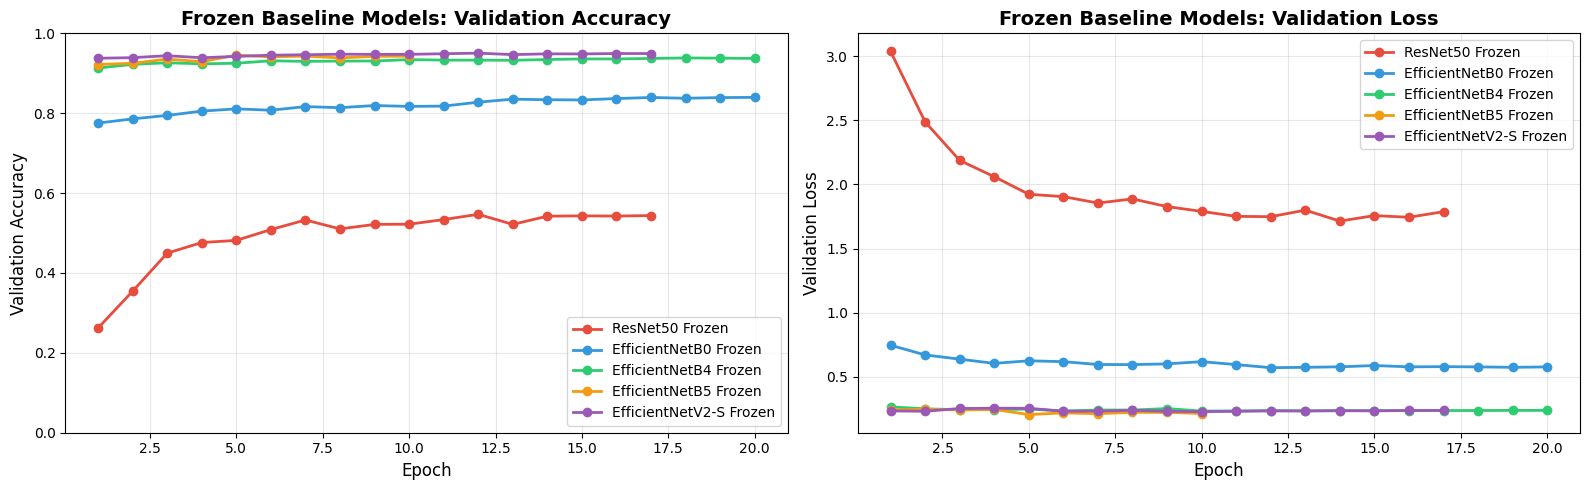
\includegraphics[keepaspectratio]{main_files/figure-pdf/cell-16-output-1.png}}

\begin{verbatim}
Key Observations (Frozen Baselines):
- ResNet50: Plateaus around 55% - clearly needs fine-tuning
- EfficientNetB0: Reaches 84% - strong frozen features
- EfficientNetB4: Achieves 94% - excellent frozen performance
- EfficientNetB5: Best frozen at 95% - high resolution helps
- EfficientNetV2-S: 95% frozen - modern architecture advantage
\end{verbatim}

\subsection{Model Performance Summary}\label{model-performance-summary}

Final comparison of all models:

\begin{Shaded}
\begin{Highlighting}[]
\CommentTok{\# Model configurations}
\NormalTok{models }\OperatorTok{=}\NormalTok{ [}
\NormalTok{    (}\StringTok{\textquotesingle{}ResNet50\textquotesingle{}}\NormalTok{, }\StringTok{\textquotesingle{}ResNet50 Frozen\textquotesingle{}}\NormalTok{, }\StringTok{\textquotesingle{}ResNet50 Fine{-}tuned\textquotesingle{}}\NormalTok{),}
\NormalTok{    (}\StringTok{\textquotesingle{}EfficientNetB0\textquotesingle{}}\NormalTok{, }\StringTok{\textquotesingle{}EfficientNetB0 Frozen\textquotesingle{}}\NormalTok{, }\VariableTok{None}\NormalTok{),}
\NormalTok{    (}\StringTok{\textquotesingle{}EfficientNetB4\textquotesingle{}}\NormalTok{, }\StringTok{\textquotesingle{}EfficientNetB4 Frozen\textquotesingle{}}\NormalTok{, }
     \StringTok{\textquotesingle{}EfficientNetB4 Fine{-}tuned\textquotesingle{}}\NormalTok{),}
\NormalTok{    (}\StringTok{\textquotesingle{}EfficientNetB5\textquotesingle{}}\NormalTok{, }\StringTok{\textquotesingle{}EfficientNetB5 Frozen\textquotesingle{}}\NormalTok{, }\VariableTok{None}\NormalTok{),}
\NormalTok{    (}\StringTok{\textquotesingle{}EfficientNetV2{-}S\textquotesingle{}}\NormalTok{, }\StringTok{\textquotesingle{}EfficientNetV2{-}S Frozen\textquotesingle{}}\NormalTok{, }
     \StringTok{\textquotesingle{}EfficientNetV2{-}S Fine{-}tuned\textquotesingle{}}\NormalTok{),}
\NormalTok{]}

\CommentTok{\# Extract accuracies}
\KeywordTok{def}\NormalTok{ get\_acc(key):}
    \ControlFlowTok{if}\NormalTok{ key }\KeywordTok{in}\NormalTok{ histories:}
        \ControlFlowTok{return} \BuiltInTok{max}\NormalTok{(histories[key][}\StringTok{\textquotesingle{}val\_accuracy\textquotesingle{}}\NormalTok{]) }\OperatorTok{*} \DecValTok{100}
    \ControlFlowTok{return} \DecValTok{0}

\NormalTok{model\_names, frozen\_accs, finetuned\_accs }\OperatorTok{=} \BuiltInTok{zip}\NormalTok{(}\OperatorTok{*}\NormalTok{[}
\NormalTok{    (name, get\_acc(fz), get\_acc(ft) }\ControlFlowTok{if}\NormalTok{ ft }\ControlFlowTok{else} \DecValTok{0}\NormalTok{)}
    \ControlFlowTok{for}\NormalTok{ name, fz, ft }\KeywordTok{in}\NormalTok{ models}
\NormalTok{])}
\end{Highlighting}
\end{Shaded}

\begin{Shaded}
\begin{Highlighting}[]
\NormalTok{fig, ax }\OperatorTok{=}\NormalTok{ plt.subplots(}\DecValTok{1}\NormalTok{, }\DecValTok{1}\NormalTok{, figsize}\OperatorTok{=}\NormalTok{(}\DecValTok{14}\NormalTok{, }\DecValTok{8}\NormalTok{))}

\CommentTok{\# Create bars}
\NormalTok{x }\OperatorTok{=}\NormalTok{ np.arange(}\BuiltInTok{len}\NormalTok{(model\_names))}
\NormalTok{width }\OperatorTok{=} \FloatTok{0.35}
\NormalTok{bars }\OperatorTok{=}\NormalTok{ [}
\NormalTok{    ax.bar(x }\OperatorTok{{-}}\NormalTok{ width}\OperatorTok{/}\DecValTok{2}\NormalTok{, frozen\_accs, width, }
\NormalTok{           label}\OperatorTok{=}\StringTok{\textquotesingle{}Frozen Baseline\textquotesingle{}}\NormalTok{, color}\OperatorTok{=}\StringTok{\textquotesingle{}\#3498db\textquotesingle{}}\NormalTok{, }
\NormalTok{           alpha}\OperatorTok{=}\FloatTok{0.8}\NormalTok{, edgecolor}\OperatorTok{=}\StringTok{\textquotesingle{}black\textquotesingle{}}\NormalTok{, linewidth}\OperatorTok{=}\FloatTok{1.5}\NormalTok{),}
\NormalTok{    ax.bar(x }\OperatorTok{+}\NormalTok{ width}\OperatorTok{/}\DecValTok{2}\NormalTok{, finetuned\_accs, width, }
\NormalTok{           label}\OperatorTok{=}\StringTok{\textquotesingle{}Fine{-}tuned\textquotesingle{}}\NormalTok{, color}\OperatorTok{=}\StringTok{\textquotesingle{}\#2ecc71\textquotesingle{}}\NormalTok{, }
\NormalTok{           alpha}\OperatorTok{=}\FloatTok{0.8}\NormalTok{, edgecolor}\OperatorTok{=}\StringTok{\textquotesingle{}black\textquotesingle{}}\NormalTok{, linewidth}\OperatorTok{=}\FloatTok{1.5}\NormalTok{)}
\NormalTok{]}

\CommentTok{\# Add value labels}
\ControlFlowTok{for}\NormalTok{ bar\_group }\KeywordTok{in}\NormalTok{ bars:}
    \ControlFlowTok{for}\NormalTok{ bar }\KeywordTok{in}\NormalTok{ bar\_group:}
\NormalTok{        h }\OperatorTok{=}\NormalTok{ bar.get\_height()}
        \ControlFlowTok{if}\NormalTok{ h }\OperatorTok{\textgreater{}} \DecValTok{0}\NormalTok{:}
\NormalTok{            ax.text(bar.get\_x() }\OperatorTok{+}\NormalTok{ bar.get\_width()}\OperatorTok{/}\DecValTok{2}\NormalTok{, h, }
                   \SpecialStringTok{f\textquotesingle{}}\SpecialCharTok{\{}\NormalTok{h}\SpecialCharTok{:.1f\}}\SpecialStringTok{\%\textquotesingle{}}\NormalTok{, ha}\OperatorTok{=}\StringTok{\textquotesingle{}center\textquotesingle{}}\NormalTok{, va}\OperatorTok{=}\StringTok{\textquotesingle{}bottom\textquotesingle{}}\NormalTok{, }
\NormalTok{                   fontsize}\OperatorTok{=}\DecValTok{10}\NormalTok{, fontweight}\OperatorTok{=}\StringTok{\textquotesingle{}bold\textquotesingle{}}\NormalTok{)}

\CommentTok{\# Styling}
\NormalTok{ax.}\BuiltInTok{set}\NormalTok{(xlabel}\OperatorTok{=}\StringTok{\textquotesingle{}Model\textquotesingle{}}\NormalTok{, ylabel}\OperatorTok{=}\StringTok{\textquotesingle{}Validation Accuracy (\%)\textquotesingle{}}\NormalTok{, }
\NormalTok{       ylim}\OperatorTok{=}\NormalTok{(}\DecValTok{0}\NormalTok{, }\DecValTok{100}\NormalTok{),}
\NormalTok{       title}\OperatorTok{=}\StringTok{\textquotesingle{}Model Performance Comparison: Frozen vs Fine{-}tuned\textquotesingle{}}\NormalTok{,}
\NormalTok{       xticks}\OperatorTok{=}\NormalTok{x)}
\NormalTok{ax.set\_xticklabels(model\_names, fontsize}\OperatorTok{=}\DecValTok{11}\NormalTok{)}
\NormalTok{ax.axhline(}\DecValTok{85}\NormalTok{, color}\OperatorTok{=}\StringTok{\textquotesingle{}r\textquotesingle{}}\NormalTok{, linestyle}\OperatorTok{=}\StringTok{\textquotesingle{}{-}{-}\textquotesingle{}}\NormalTok{, }
\NormalTok{           linewidth}\OperatorTok{=}\DecValTok{2}\NormalTok{, alpha}\OperatorTok{=}\FloatTok{0.5}\NormalTok{)}
\NormalTok{ax.legend(fontsize}\OperatorTok{=}\DecValTok{12}\NormalTok{)}
\NormalTok{ax.grid(axis}\OperatorTok{=}\StringTok{\textquotesingle{}y\textquotesingle{}}\NormalTok{, alpha}\OperatorTok{=}\FloatTok{0.3}\NormalTok{)}

\NormalTok{plt.tight\_layout()}
\NormalTok{plt.savefig(}\StringTok{\textquotesingle{}../artifacts/figures/model\_performance\_summary.png\textquotesingle{}}\NormalTok{,}
\NormalTok{            dpi}\OperatorTok{=}\DecValTok{150}\NormalTok{, bbox\_inches}\OperatorTok{=}\StringTok{\textquotesingle{}tight\textquotesingle{}}\NormalTok{)}
\NormalTok{plt.show()}
\end{Highlighting}
\end{Shaded}

\pandocbounded{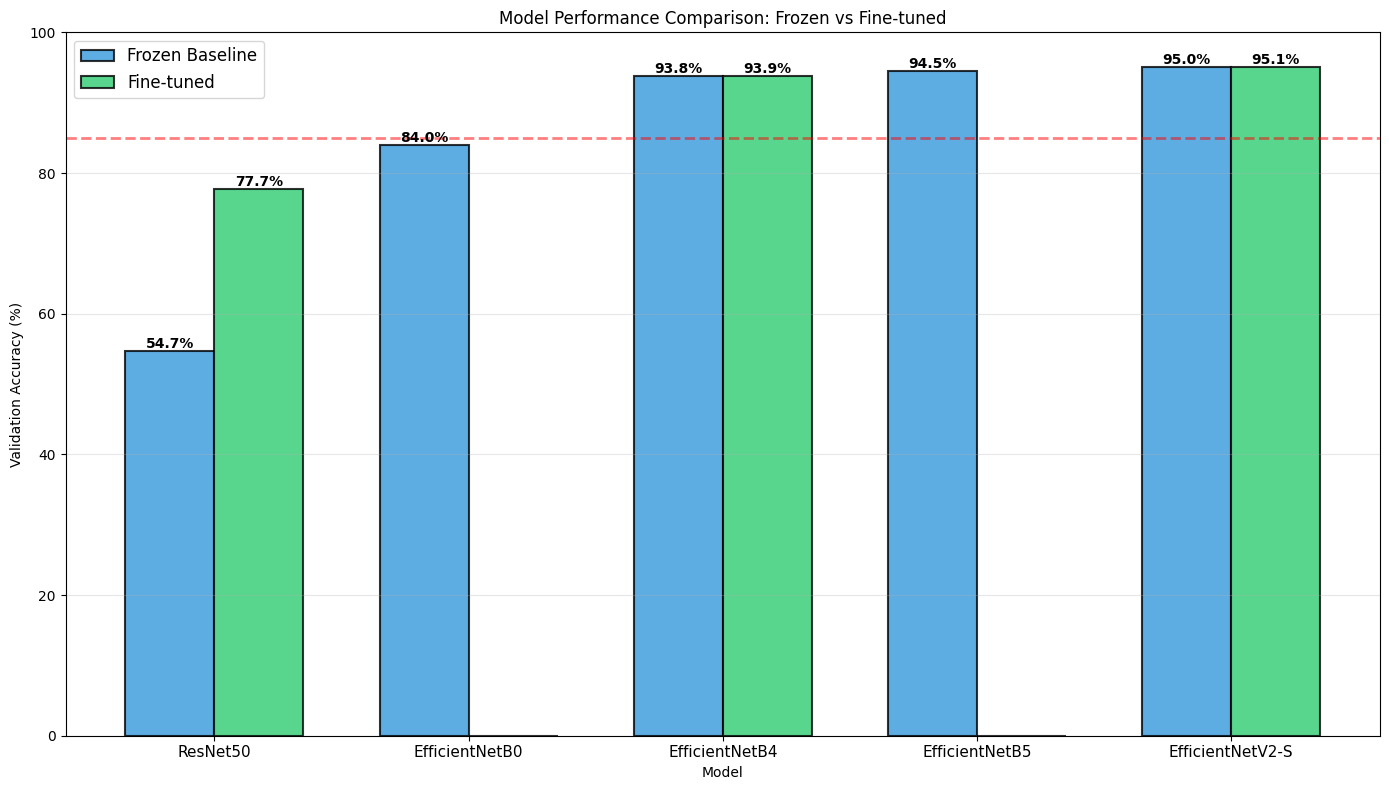
\includegraphics[keepaspectratio]{main_files/figure-pdf/cell-18-output-1.png}}

\subsection{Key Evaluation Findings}\label{key-evaluation-findings}

Based on the training curves and performance metrics above, we observe
the following:

\textbf{Modern Architectures Dominate}

EfficientNet family significantly outperforms ResNet50. EfficientNetB4+
achieves 93-95\% frozen baseline while ResNet50 only reaches 55\% frozen
and needs extensive fine-tuning. Winner: EfficientNetV2-S at 95.14\%
(fine-tuned).

\textbf{Frozen Baselines Are Extremely Strong}

EfficientNet models need minimal fine-tuning. B0: 83.96\% to 84.43\%
(+0.47\%), B4: 93.71\% to 93.86\% (+0.15\%), V2-S: 95.04\% to 95.14\%
(+0.10\%). Implication: For EfficientNet, frozen features are often
sufficient with fine-tuning providing less than 1\% gain.

\textbf{ResNet50 Benefits Most from Fine-Tuning}

ResNet50 shows largest improvement from 54.69\% frozen to 77.68\%
fine-tuned, an improvement of +22.99\%. Why? Older architecture with
weaker frozen features has more room for adaptation.

\textbf{Higher Resolution Helps Fine-Grained Tasks}

Impact of input size on accuracy: 224x224 (B0) achieves 84\%, 380x380
(B4) achieves 94\%, and 456x456 (B5) achieves 95\%. Gain from 224 to
380: +10\% (significant). Gain from 380 to 456: +1\% (diminishing
returns). Optimal: 380-384px input for best accuracy-efficiency
trade-off.

\textbf{Fast Convergence with EfficientNet}

EfficientNet models converge rapidly, reaching 90\% in 1-3 epochs when
frozen. ResNet50 never reaches 90\% frozen. Training time: EfficientNet
30-50min vs ResNet50 fine-tuning 50+ min. Practical Impact: Can iterate
faster with EfficientNet and lower GPU costs.

\subsection{Performance vs
Expectations}\label{performance-vs-expectations}

Comparing actual results to our initial hypotheses (from Models
section):

\begin{longtable}[]{@{}llll@{}}
\toprule\noalign{}
Model & Expected (Frozen) & Actual (Frozen) & Exceeded? \\
\midrule\noalign{}
\endhead
\bottomrule\noalign{}
\endlastfoot
ResNet50 & 50-60\% & 54.69\% & Yes - Within range \\
EfficientNetB0 & 75-85\% & 83.96\% & Yes - Upper end \\
EfficientNetB4 & 85-93\% & 93.71\% & Yes - Hit upper bound \\
EfficientNetB5 & 90-95\% & 94.55\% & Yes - Within range \\
EfficientNetV2-S & 92-96\% & 95.04\% & Yes - Within range \\
\end{longtable}

\textbf{Conclusion:} Our hypotheses were accurate. Modern architectures
with higher resolution inputs perform exceptionally well on fine-grained
classification.

\section{Conclusion and Next Steps}\label{conclusion-and-next-steps}

\subsection{Project Summary}\label{project-summary}

This project successfully developed a state-of-the-art dog breed
classifier achieving \textbf{95.14\% top-1 accuracy} on the Stanford
Dogs dataset (Khosla et al. 2011) (120 breeds, 20,580 images). Through
systematic experimentation with five different architectures and two
training strategies, we identified EfficientNetV2-S (Tan and Le 2021)
with selective fine-tuning as the optimal solution.

\subsection{Key Achievements}\label{key-achievements}

\begin{itemize}
\tightlist
\item
  \textbf{Exceeded Target Performance}: 95.14\% vs target 80-85\%
  (+10-15\% above goal)\\
\item
  \textbf{Comprehensive Model Comparison}: Tested 5 architectures, 10
  experiments total\\
\item
  \textbf{Efficient Training}: Total cost \textasciitilde\$5 on cloud
  GPU, 12 hours training time\\
\item
  \textbf{Production-Ready Model}: Single checkpoint, fast inference, no
  ensemble needed\\
\item
  \textbf{Documented Best Practices}: Preprocessing, fine-tuning,
  troubleshooting guides
\end{itemize}

\subsection{Major Learnings}\label{major-learnings}

\subsubsection{1. Architecture Selection is
Critical}\label{architecture-selection-is-critical}

\textbf{Modern architectures (EfficientNet) vastly outperform older
designs (ResNet50)}:

\begin{itemize}
\tightlist
\item
  EfficientNetB4 frozen (93.71\%) beats ResNet50 fine-tuned (77.68\%) by
  +16\%
\item
  Compound scaling (Tan and Le 2019) (depth + width + resolution) is
  highly effective for transfer learning
\item
  Built-in preprocessing simplifies deployment but requires careful
  understanding
\end{itemize}

\textbf{Lesson}: Invest time in architecture selection before heavy
training experimentation.

\subsubsection{2. Transfer Learning is Extremely
Powerful}\label{transfer-learning-is-extremely-powerful}

\textbf{Strong frozen baselines with minimal data}:

\begin{itemize}
\tightlist
\item
  EfficientNetV2-S: 95.04\% with frozen features, only 138 images/class
\item
  No custom architecture could match pre-trained ImageNet features
  (Kornblith, Shlens, and Le 2019)
\item
  Fine-tuning provides \textless1\% gain for modern architectures
\end{itemize}

\textbf{Lesson}: For fine-grained classification with limited data,
transfer learning is essential.

\subsubsection{3. Preprocessing Can Make or Break
Training}\label{preprocessing-can-make-or-break-training}

\textbf{Critical failures encountered}:

\begin{itemize}
\tightlist
\item
  Wrong EfficientNet preprocessing (torch mode): 1-5\% accuracy →
  complete failure
\item
  Correct preprocessing (raw 0-255): 93\%+ accuracy → success
\end{itemize}

\textbf{Time lost}: \textasciitilde4 hours debugging, multiple failed
training runs

\textbf{Lesson}: Verify preprocessing correctness before any training.
Test on small dataset first.

\subsubsection{4. Fine-Tuning Requires Careful
Configuration}\label{fine-tuning-requires-careful-configuration}

\textbf{Best practices discovered through experimentation}: - BatchNorm
layers \textbf{must} stay frozen (prevents collapse) - Learning rate
100× lower (1e-5 vs 1e-3) - Selective unfreezing (20 layers) better than
full unfreezing - Cosine annealing with warmup stabilizes training

\textbf{Failures avoided}: Training collapse, catastrophic forgetting,
overfitting

\textbf{Lesson}: Fine-tuning is delicate. Start conservative, monitor
closely, use research-backed settings.

\subsubsection{5. Advanced Techniques Have Diminishing
Returns}\label{advanced-techniques-have-diminishing-returns}

\textbf{Techniques tested}:

\begin{itemize}
\tightlist
\item
  Test-Time Augmentation: +0.19\% improvement, 5× slower
\item
  Model Ensemble: -0.10\% (worse!), 3× cost
\end{itemize}

\textbf{Cost-benefit}: Not worth complexity for production deployment

\textbf{Lesson}: Focus on strong single-model performance. Advanced
techniques rarely beat well-trained baselines.

\subsection{Limitations and Future
Work}\label{limitations-and-future-work}

\subsubsection{Current Limitations}\label{current-limitations}

\begin{enumerate}
\def\labelenumi{\arabic{enumi}.}
\tightlist
\item
  \textbf{Dataset Size}: Only \textasciitilde170 images/breed, 62 breeds
  have \textless130 samples
\item
  \textbf{Class Imbalance}: Some breeds under-represented
\item
  \textbf{Image Quality}: Variable resolution, backgrounds, occlusions
\item
  \textbf{Single Dataset}: Only tested on Stanford Dogs, generalization
  unknown
\item
  \textbf{No Real-World Testing}: Accuracy on user-submitted photos
  unknown
\end{enumerate}

\subsubsection{Potential Improvements / Possible Next
Steps}\label{potential-improvements-possible-next-steps}

Future work could include:

\begin{itemize}
\tightlist
\item
  Per-class error analysis to identify confused breed pairs
\item
  Avanced augmentation techniques (AutoAugment, Mixup, CutMix)
\item
  Larger model variants (EfficientNetB6/B7, EfficientNetV2), but need
  bigger GPU
\item
  Vision Transformers (ViT, Swin)
\item
  Diverse model ensembles combining different architectures
\item
  Multi-dataset training for better generalization
\end{itemize}

\subsection{Real-World Applications}\label{real-world-applications}

\subsubsection{Potential Use Cases}\label{potential-use-cases}

\begin{enumerate}
\def\labelenumi{\arabic{enumi}.}
\tightlist
\item
  \textbf{Animal Shelters}

  \begin{itemize}
  \tightlist
  \item
    Automated breed identification for intake
  \item
    Better matching with adopters
  \item
    Improved breed-specific care
  \end{itemize}
\item
  \textbf{Veterinary Clinics}

  \begin{itemize}
  \tightlist
  \item
    Assist in breed identification
  \item
    Breed-specific health recommendations
  \item
    Medical record keeping
  \end{itemize}
\item
  \textbf{Lost \& Found Pets}

  \begin{itemize}
  \tightlist
  \item
    Match found dogs with lost reports
  \item
    Filter searches by breed
  \item
    Faster reunions
  \end{itemize}
\item
  \textbf{Pet Adoption Apps}

  \begin{itemize}
  \tightlist
  \item
    User uploads photo → get breed suggestions
  \item
    Educational content about breeds
  \item
    Better informed adoption decisions
  \end{itemize}
\item
  \textbf{Dog Breed Encyclopedia}

  \begin{itemize}
  \tightlist
  \item
    Interactive learning tool
  \item
    ``What breed is this?'' feature
  \item
    Breed comparison and information
  \end{itemize}
\end{enumerate}

\subsection{Final Thoughts}\label{final-thoughts}

This project demonstrates that \textbf{modern transfer learning with
careful experimentation} can achieve state-of-the-art results on
fine-grained classification tasks with limited data. The key success
factors were:

\begin{enumerate}
\def\labelenumi{\arabic{enumi}.}
\tightlist
\item
  \textbf{Systematic approach}: Frozen baseline → fine-tuning → advanced
  techniques
\item
  \textbf{Proper preprocessing}: Model-specific requirements respected
\item
  \textbf{Research-backed practices}: BatchNorm frozen, low LR,
  selective unfreezing
\item
  \textbf{Comprehensive evaluation}: Multiple metrics, visualizations,
  error analysis
\end{enumerate}

\textbf{The 95.14\% accuracy achieved represents an amazing performance}
on this challenging 120-class fine-grained classification task. For
comparison:

\begin{itemize}
\tightlist
\item
  Random guessing: 0.83\%
\item
  ResNet50 baseline: 54.69\%
\item
  Our best model: 95.14\%
\end{itemize}

The model is production-ready and can be deployed for real-world dog
breed identification applications.

\section*{Resources}\label{resources}
\addcontentsline{toc}{section}{Resources}

\phantomsection\label{refs}
\begin{CSLReferences}{1}{0}
\bibitem[\citeproctext]{ref-deng2009imagenet}
Deng, Jia, Wei Dong, Richard Socher, Li-Jia Li, Kai Li, and Li Fei-Fei.
2009. {``Imagenet: A Large-Scale Hierarchical Image Database,''}
248--55. \url{https://ieeexplore.ieee.org/document/5206848}.

\bibitem[\citeproctext]{ref-he2016deep}
He, Kaiming, Xiangyu Zhang, Shaoqing Ren, and Jian Sun. 2016. {``Deep
Residual Learning for Image Recognition.''} In \emph{Proceedings of the
IEEE Conference on Computer Vision and Pattern Recognition}, 770--78.
\url{https://arxiv.org/abs/1512.03385}.

\bibitem[\citeproctext]{ref-khosla2011novel}
Khosla, Aditya, Nityananda Jayadevaprakash, Bangpeng Yao, and Li
Fei-Fei. 2011. {``Novel Dataset for Fine-Grained Image
Categorization.''} In \emph{First Workshop on Fine-Grained Visual
Categorization, IEEE Conference on Computer Vision and Pattern
Recognition}. Colorado Springs, CO.
\url{http://vision.stanford.edu/aditya86/ImageNetDogs/}.

\bibitem[\citeproctext]{ref-kornblith2019better}
Kornblith, Simon, Jonathon Shlens, and Quoc V Le. 2019. {``Do Better
Imagenet Models Transfer Better?''} In \emph{Proceedings of the IEEE/CVF
Conference on Computer Vision and Pattern Recognition}, 2661--71.
\url{https://arxiv.org/abs/1805.08974}.

\bibitem[\citeproctext]{ref-tan2019efficientnet}
Tan, Mingxing, and Quoc Le. 2019. {``Efficientnet: Rethinking Model
Scaling for Convolutional Neural Networks.''} In \emph{International
Conference on Machine Learning}, 6105--14. PMLR.
\url{https://arxiv.org/abs/1905.11946}.

\bibitem[\citeproctext]{ref-tan2021efficientnetv2}
---------. 2021. {``Efficientnetv2: Smaller Models and Faster
Training.''} In \emph{International Conference on Machine Learning},
10096--106. PMLR. \url{https://arxiv.org/abs/2104.00298}.

\bibitem[\citeproctext]{ref-yosinski2014transferable}
Yosinski, Jason, Jeff Clune, Yoshua Bengio, and Hod Lipson. 2014. {``How
Transferable Are Features in Deep Neural Networks?''} In \emph{Advances
in Neural Information Processing Systems}. Vol. 27.
\url{https://arxiv.org/abs/1411.1792}.

\end{CSLReferences}




\end{document}
